% Options for packages loaded elsewhere
\PassOptionsToPackage{unicode}{hyperref}
\PassOptionsToPackage{hyphens}{url}
%
\documentclass[
]{book}
\usepackage{amsmath,amssymb}
\usepackage{iftex}
\ifPDFTeX
  \usepackage[T1]{fontenc}
  \usepackage[utf8]{inputenc}
  \usepackage{textcomp} % provide euro and other symbols
\else % if luatex or xetex
  \usepackage{unicode-math} % this also loads fontspec
  \defaultfontfeatures{Scale=MatchLowercase}
  \defaultfontfeatures[\rmfamily]{Ligatures=TeX,Scale=1}
\fi
\usepackage{lmodern}
\ifPDFTeX\else
  % xetex/luatex font selection
\fi
% Use upquote if available, for straight quotes in verbatim environments
\IfFileExists{upquote.sty}{\usepackage{upquote}}{}
\IfFileExists{microtype.sty}{% use microtype if available
  \usepackage[]{microtype}
  \UseMicrotypeSet[protrusion]{basicmath} % disable protrusion for tt fonts
}{}
\makeatletter
\@ifundefined{KOMAClassName}{% if non-KOMA class
  \IfFileExists{parskip.sty}{%
    \usepackage{parskip}
  }{% else
    \setlength{\parindent}{0pt}
    \setlength{\parskip}{6pt plus 2pt minus 1pt}}
}{% if KOMA class
  \KOMAoptions{parskip=half}}
\makeatother
\usepackage{xcolor}
\usepackage{color}
\usepackage{fancyvrb}
\newcommand{\VerbBar}{|}
\newcommand{\VERB}{\Verb[commandchars=\\\{\}]}
\DefineVerbatimEnvironment{Highlighting}{Verbatim}{commandchars=\\\{\}}
% Add ',fontsize=\small' for more characters per line
\usepackage{framed}
\definecolor{shadecolor}{RGB}{248,248,248}
\newenvironment{Shaded}{\begin{snugshade}}{\end{snugshade}}
\newcommand{\AlertTok}[1]{\textcolor[rgb]{0.94,0.16,0.16}{#1}}
\newcommand{\AnnotationTok}[1]{\textcolor[rgb]{0.56,0.35,0.01}{\textbf{\textit{#1}}}}
\newcommand{\AttributeTok}[1]{\textcolor[rgb]{0.13,0.29,0.53}{#1}}
\newcommand{\BaseNTok}[1]{\textcolor[rgb]{0.00,0.00,0.81}{#1}}
\newcommand{\BuiltInTok}[1]{#1}
\newcommand{\CharTok}[1]{\textcolor[rgb]{0.31,0.60,0.02}{#1}}
\newcommand{\CommentTok}[1]{\textcolor[rgb]{0.56,0.35,0.01}{\textit{#1}}}
\newcommand{\CommentVarTok}[1]{\textcolor[rgb]{0.56,0.35,0.01}{\textbf{\textit{#1}}}}
\newcommand{\ConstantTok}[1]{\textcolor[rgb]{0.56,0.35,0.01}{#1}}
\newcommand{\ControlFlowTok}[1]{\textcolor[rgb]{0.13,0.29,0.53}{\textbf{#1}}}
\newcommand{\DataTypeTok}[1]{\textcolor[rgb]{0.13,0.29,0.53}{#1}}
\newcommand{\DecValTok}[1]{\textcolor[rgb]{0.00,0.00,0.81}{#1}}
\newcommand{\DocumentationTok}[1]{\textcolor[rgb]{0.56,0.35,0.01}{\textbf{\textit{#1}}}}
\newcommand{\ErrorTok}[1]{\textcolor[rgb]{0.64,0.00,0.00}{\textbf{#1}}}
\newcommand{\ExtensionTok}[1]{#1}
\newcommand{\FloatTok}[1]{\textcolor[rgb]{0.00,0.00,0.81}{#1}}
\newcommand{\FunctionTok}[1]{\textcolor[rgb]{0.13,0.29,0.53}{\textbf{#1}}}
\newcommand{\ImportTok}[1]{#1}
\newcommand{\InformationTok}[1]{\textcolor[rgb]{0.56,0.35,0.01}{\textbf{\textit{#1}}}}
\newcommand{\KeywordTok}[1]{\textcolor[rgb]{0.13,0.29,0.53}{\textbf{#1}}}
\newcommand{\NormalTok}[1]{#1}
\newcommand{\OperatorTok}[1]{\textcolor[rgb]{0.81,0.36,0.00}{\textbf{#1}}}
\newcommand{\OtherTok}[1]{\textcolor[rgb]{0.56,0.35,0.01}{#1}}
\newcommand{\PreprocessorTok}[1]{\textcolor[rgb]{0.56,0.35,0.01}{\textit{#1}}}
\newcommand{\RegionMarkerTok}[1]{#1}
\newcommand{\SpecialCharTok}[1]{\textcolor[rgb]{0.81,0.36,0.00}{\textbf{#1}}}
\newcommand{\SpecialStringTok}[1]{\textcolor[rgb]{0.31,0.60,0.02}{#1}}
\newcommand{\StringTok}[1]{\textcolor[rgb]{0.31,0.60,0.02}{#1}}
\newcommand{\VariableTok}[1]{\textcolor[rgb]{0.00,0.00,0.00}{#1}}
\newcommand{\VerbatimStringTok}[1]{\textcolor[rgb]{0.31,0.60,0.02}{#1}}
\newcommand{\WarningTok}[1]{\textcolor[rgb]{0.56,0.35,0.01}{\textbf{\textit{#1}}}}
\usepackage{longtable,booktabs,array}
\usepackage{calc} % for calculating minipage widths
% Correct order of tables after \paragraph or \subparagraph
\usepackage{etoolbox}
\makeatletter
\patchcmd\longtable{\par}{\if@noskipsec\mbox{}\fi\par}{}{}
\makeatother
% Allow footnotes in longtable head/foot
\IfFileExists{footnotehyper.sty}{\usepackage{footnotehyper}}{\usepackage{footnote}}
\makesavenoteenv{longtable}
\usepackage{graphicx}
\makeatletter
\def\maxwidth{\ifdim\Gin@nat@width>\linewidth\linewidth\else\Gin@nat@width\fi}
\def\maxheight{\ifdim\Gin@nat@height>\textheight\textheight\else\Gin@nat@height\fi}
\makeatother
% Scale images if necessary, so that they will not overflow the page
% margins by default, and it is still possible to overwrite the defaults
% using explicit options in \includegraphics[width, height, ...]{}
\setkeys{Gin}{width=\maxwidth,height=\maxheight,keepaspectratio}
% Set default figure placement to htbp
\makeatletter
\def\fps@figure{htbp}
\makeatother
\setlength{\emergencystretch}{3em} % prevent overfull lines
\providecommand{\tightlist}{%
  \setlength{\itemsep}{0pt}\setlength{\parskip}{0pt}}
\setcounter{secnumdepth}{5}
\usepackage{booktabs}
\usepackage{array}
\usepackage{longtable}  
\usepackage{lmodern}    
\usepackage{graphicx}
\usepackage{amsmath}
\usepackage{hyperref}
\hypersetup{
    colorlinks=true,
    linkcolor=DarkBlue,
    filecolor=DarkGreen,
    urlcolor=DarkRed,
    citecolor=DarkGreen
%    pdftitle={Overleaf Example},
    pdfpagemode=FullScreen,
    }
\usepackage{booktabs}
\usepackage{longtable}
\usepackage{array}
\usepackage{multirow}
\usepackage{wrapfig}
\usepackage{float}
\usepackage{colortbl}
\usepackage{pdflscape}
\usepackage{tabu}
\usepackage{threeparttable}
\usepackage{threeparttablex}
\usepackage[normalem]{ulem}
\usepackage{makecell}
\usepackage{xcolor}
\usepackage{caption}
\usepackage{anyfontsize}
\ifLuaTeX
  \usepackage{selnolig}  % disable illegal ligatures
\fi
\usepackage[]{natbib}
\bibliographystyle{plainnat}
\usepackage{bookmark}
\IfFileExists{xurl.sty}{\usepackage{xurl}}{} % add URL line breaks if available
\urlstyle{same}
\hypersetup{
  pdftitle={Análise Exploratória de Dados},
  pdfauthor={Gabriela Scarpini e Victor Fossaluza},
  hidelinks,
  pdfcreator={LaTeX via pandoc}}

\title{Análise Exploratória de Dados}
\author{Gabriela Scarpini e Victor Fossaluza}
\date{2025-05-03}

\begin{document}
\maketitle

{
\setcounter{tocdepth}{1}
\tableofcontents
}
\chapter{Introdução}\label{intro}

\section{Apresentação}\label{apresentauxe7uxe3o}

Esse material está em fase inicial de desenvolvimento e será utilizado para apoiar as aulas de MAE0111 - Análise Exploratória de Dados.

O objetivo principal da apostila é funcionar como um resumo e auxiliar os estudantes na compreensão dos conceitos teóricos, com capítulos curtos e por meio de exercícios ao final de cada capítulo.

Comentários e correções podem ser enviadas para \url{gabi.scarpini@usp.br}.

\begin{center}\rule{0.5\linewidth}{0.5pt}\end{center}

\section{Programa}\label{programa}

\begin{enumerate}
\def\labelenumi{\arabic{enumi}.}
\tightlist
\item
  A profissão de Estatística. A Estatística como metodologia de todas as ciências experimentais. O mercado de trabalho. O perfil profissional do Estatístico. A Estatística acadêmica: pós-graduação e pesquisa.
\item
  Apresentação de problemas reais analisados no CEA -- Centro de Estatística Aplicada da USP, com ênfase na análise descritiva dos dados. Conclusões dos estudos.
\item
  Estatística descritiva e inferência estatística, tipos de dados, bancos de dados, ordem de grandeza, precisão e arredondamento de dados quantitativos, proporções e porcentagens, taxas e números índices, sugestões para construção e apresentação de gráficos e tabelas.
\item
  Representação gráfica e tabular da distribuição de dados: tabelas de frequências, gráficos de barras e do tipo ``torta'', histogramas, densidade suavizada e função de distribuição empírica.
\item
  Medidas-resumo: medidas de posição, de dispersão, de assimetria e curtose, gráficos do tipo boxplot.
\item
  Modelos para distribuições de frequências: gráficos de probabilidade.
\item
  Associação entre variáveis qualitativas: tabelas de contingência de dupla entrada, coeficientes de associação, sensibilidade e especificidade, risco relativo, razão de chances, tabelas de contingência de múltiplas entradas.
\item
  Associação entre variáveis quantitativas: gráficos de dispersão, covariância, correlação linear, matriz de covariâncias, matriz de correlações.
\item
  Associação entre uma variável quantitativa e uma variável qualitativa: homogeneidade de distribuições, gráficos de médias, gráficos de perfis.
\item
  Outros tópicos: elaboração de relatórios técnicos, uso do aplicativo R, dashboards.
\end{enumerate}

\begin{center}\rule{0.5\linewidth}{0.5pt}\end{center}

\section{Bibliografia}\label{bibliografia}

\begin{itemize}
\item
  Damiani, A., Milz, B., Lente, C., Falbel, D., Correa, F., Trecenti, J., Luduvice, N., Lacerda, T., Amorim, W. Ciência de Dados em R, Curso-R \href{https://livro.curso-r.com/}{link}
\item
  Peng, R.D. Exploratory Data Analysis with R, Leanpub. \href{https://bookdown.org/rdpeng/exdata/}{link}
\item
  Mayer, F.P, Bonat, W.H., Zeviani, W.M., Krainski, E.T., Ribeiro Jr, P.J. Estatística Computacional com R. \href{http://cursos.leg.ufpr.br/ecr/index.html}{link}
\item
  Grolemund, G. Wickham, H. R for Data Science. \href{https://r4ds.hadley.nz/}{link} (versão em português: \href{https://pt.r4ds.hadley.nz/}{link})
\item
  Chang, W. R Graphics Cookbook, 2nd edition. \href{Chang,\%20W.\%20R\%20Graphics\%20Cookbook,\%202nd\%20edition.}{link}
\item
  Grolemund, G. Hands-On Programming with R. \href{https://jjallaire.github.io/hopr/}{link}
\end{itemize}

\begin{center}\rule{0.5\linewidth}{0.5pt}\end{center}

\section{Bibliografia Jupiterweb}\label{bibliografia-jupiterweb}

\begin{itemize}
\item
  Morettin, P. A., Bussab, W. O. (2017). Estatística Básica. 9a edição. Saraiva Educação SA.
\item
  Wickham, H., Grolemund, G. (2017). R for data science: import, tidy, transform, visualize, and model data, O'Reilly Media, Inc.~\href{https://r4ds.hadley.nz/}{link}
\item
  Tukey,J. W. (1977). Exploratory Data Analysis. Reading: Addison Wesley.
\item
  Cairo, A. (2016). The truthful art: Data, charts, and maps for communication. New Riders.
\item
  Tufte, E. R. (1983). The Visual Display of Quantitative Information, Cheshire: Graphics Press.
\item
  Few, S. (2012). Show Me the Numbers: Designing Tables and Graphs to Enlighten, 2a ed.~Analytics Press.
\end{itemize}

\begin{center}\rule{0.5\linewidth}{0.5pt}\end{center}

\section{Bibliografia Complementar}\label{bibliografia-complementar}

\begin{itemize}
\item
  Relatórios do CEA -- Centro de Estatística Aplicada -- USP.
\item
  Magalhães, M. N, de Lima, A. C. P. (2015). Noções de Probabilidade e Estatística. 7a edição. Editora da Universidade de São Paulo.
\item
  Murteira, B. F. J., Black, G. H. J.. (1983). Análise Exploratória de Dados - Estatística Descritiva, Lisboa: McGraw Hill.
\item
  Wexler, S., Shaffer, J., \& Cotgreave, A. (2017). The big book of dashboards: visualizing your data using real-world business scenarios. John Wiley \& Sons.
\item
  ChambersJ. M., ClevelandW. S., Tukey, P. A.. (1983). Graphical Methods for Data Analysis. Boston: Duxbury Press.
\item
  W. M. Cleveland. (1993). Visualizing Data, Summit, New Jersey: Hobart Press.
\item
  W. M. Cleveland. (1994). The Elements of Graphing Data, Summit: Hobart Press.
\end{itemize}

\begin{center}\rule{0.5\linewidth}{0.5pt}\end{center}

\chapter{Conceitos básicos de Análise Exploratória de Dados}\label{conceitos_aed1}

\section{O que significa algo ser ``aleatório''?}\label{o-que-significa-algo-ser-aleatuxf3rio}

\begin{itemize}
\tightlist
\item
  \textbf{Aleatório} \emph{(Google - Oxford Languages)}\\
  \emph{(adjetivo)}\\
\end{itemize}

\begin{enumerate}
\def\labelenumi{\arabic{enumi}.}
\tightlist
\item
  que depende das circunstâncias, do acaso; casual, fortuito, contingente.\\
\item
  (física) referente a fenômenos físicos para os quais as variáveis tomam valores segundo uma determinada lei de probabilidade (p.ex., o movimento browniano).
\end{enumerate}

\begin{itemize}
\tightlist
\item
  \textbf{Experimento Aleatório} \emph{(The Concise Encyclopedia of Statistics, pp 430--433)}
\end{itemize}

Um experimento em que o resultado não é previsível com antecedência é chamado de experimento aleatório. Um experimento aleatório pode ser caracterizado da seguinte forma:\\
1. É possível descrever o conjunto de todos os resultados possíveis (chamado espaço amostral do experimento aleatório).\\
2. Não é possível prever o resultado com certeza.\\
3. É possível associar cada resultado possível a uma probabilidade de ocorrência.

\begin{center}\rule{0.5\linewidth}{0.5pt}\end{center}

\section{O que é Probabilidade?}\label{o-que-uxe9-probabilidade}

\begin{itemize}
\tightlist
\item
  \textbf{Probabilidade} \emph{(Google - Oxford Languages)}\\
  \emph{(substantivo feminino)}\\
\end{itemize}

\begin{enumerate}
\def\labelenumi{\arabic{enumi}.}
\tightlist
\item
  perspectiva favorável de que algo venha a ocorrer; possibilidade, chance.
  ``há pouca probabilidade de chuva''\\
\item
  grau de segurança com que se pode esperar a realização de um evento, determinado pela frequência relativa dos eventos do mesmo tipo numa série de tentativas.
\end{enumerate}

\begin{itemize}
\tightlist
\item
  \textbf{Probabilidade} \emph{(The Concise Encyclopedia of Statistics, pp 430--433)}
\end{itemize}

Podemos definir a probabilidade de um evento usando as frequências relativas ou por meio de uma abordagem axiomática.

Na primeira abordagem, supomos que um experimento aleatório é repetido muitas vezes nas mesmas condições. Para cada evento \(A\) definido no espaço amostral \(\Omega\), definimos \(n_A\) como o número de vezes que o evento \(A\) ocorreu durante as primeiras \(n\) repetições do experimento. Neste caso, a probabilidade do evento \(A\), denotada por \(P(A)\), é definido por:
\[P(A) = \lim_{n\rightarrow\infty} \frac{n_A}{n}~,\]

o que significa que \(P(A)\) é definido como o limite relativo ao número de vezes que o evento \(A\) ocorreu relativo ao número total de repetições.

Na segunda abordagem, para cada evento \(A\), aceitamos que existe uma probabilidade de \(A\), \(P(A)\), satisfazendo os três axiomas a seguir:\\
1. \(0\leq P(A)\leq 1\),\\
2. \(P(\Omega)=1\),\\
3. Para cada sequência de eventos mutuamente exclusivos \(A_1,A_2,\ldots\) (isto é, eventos tais que \(A_i \cap A_j = \emptyset\) se \(i \neq j\)):
\[ P\left(\bigcup_{i=1}^{\infty} A_i\right) = \sum_{i=1}^{\infty} P(Ai)~.\]
---

\subsection{Interpretações de Probabilidade}\label{interpretauxe7uxf5es-de-probabilidade}

\begin{itemize}
\tightlist
\item
  \textbf{Interpretação Clássica} (De Moivre, Laplace)

  \begin{itemize}
  \tightlist
  \item
    baseia-se na equiprobabilidade dos resultados;
  \item
    \(P(A) = \frac{|A|}{|\Omega|}\).
  \item
    \textbf{Exemplo:} um lançamento de moeda, \(A\) = ``cara'', \(P(A) = \frac{1}{2}\).
  \end{itemize}
\end{itemize}

\(~\)

\begin{itemize}
\tightlist
\item
  \textbf{Interpretação Frequentista} (Venn, von Mises, Reichenbach, etc.)

  \begin{itemize}
  \tightlist
  \item
    quase unânime na primeira metade do século XX e ainda é a mais aceita;
  \item
    baseia-se na regularidade das frequências relativas (lei dos grandes números);
  \item
    \(P(A) = lim \frac{A_n}{n}\), onde \(A_n\) é o número de ocorrências de \(A\) em \(n\) realizações \emph{idênticas e independentes} do experimento;
  \item
    Supõe que é possível repetir indefinidamente o experimento nas mesmas circustâncias.
  \item
    \textbf{Exemplo:} um lançamento de moeda, \(A\) = ``cara''.
  \end{itemize}
\end{itemize}

\begin{center}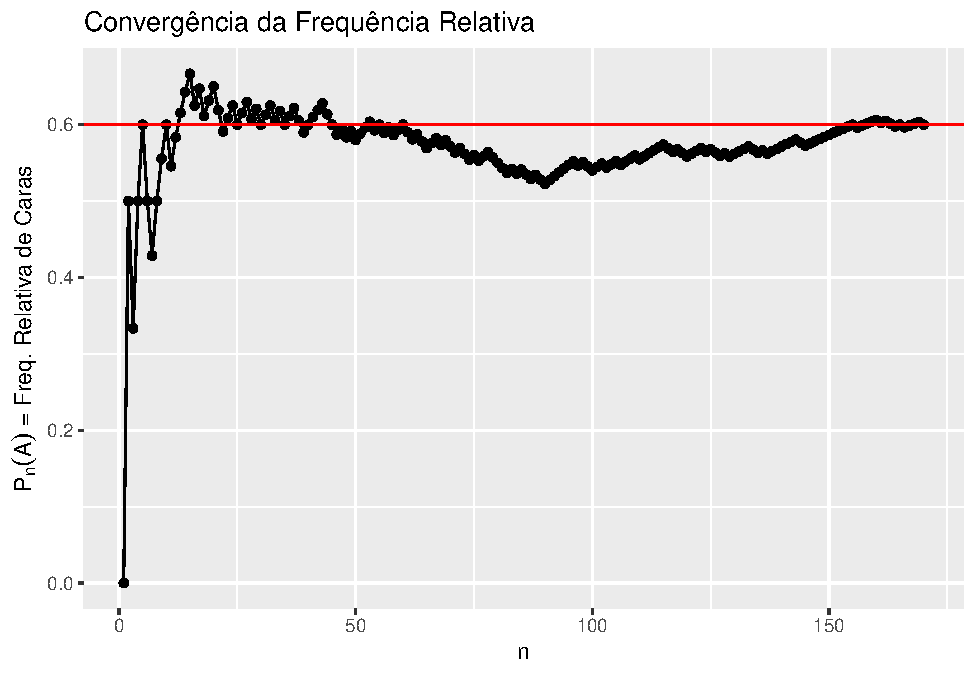
\includegraphics{AED_files/figure-latex/LGN-1} \end{center}

\(~\)

\begin{itemize}
\tightlist
\item
  \textbf{Interpretação Lógica} (Keynes, Jeffreys, Carnap, etc.)

  \begin{itemize}
  \tightlist
  \item
    medida de ``vínculo parcial'' entre uma evidência e uma hipótese;
  \item
    baseia-se em relações objetivas entre proposições.
  \item
    \textbf{Exemplo:} considere duas proposições: ``até agora todos os lançamentos resultaram em cara'' e ``será realizado um novo lançamento''. Pode-se afirmar que ``provavelmente o resultado do novo lançamento será cara''.
  \end{itemize}
\end{itemize}

\begin{itemize}
\tightlist
\item
  \textbf{Interpretação Subjetivista} (Ramsey, de Finetti, Savage, etc)

  \begin{itemize}
  \tightlist
  \item
    probabilidade como medida subjetiva de crença;
  \item
    baseada na experiência de cada indivíduo, portanto única.
  \item
    \textbf{Exemplo:} suponha que Bruno lançou uma moeda 3 vezes e todos os resultados foram cara. Esse indivíduo, em posse dessa informação, pode acreditar que o resultado cara é mais provável que coroa. Contudo, quando pergunta sobre a probabilidade de cara ao seu colega Olavo, ignorante com relação a moeda, ele responde que é 1/2.
  \end{itemize}
\end{itemize}

\begin{center}\rule{0.5\linewidth}{0.5pt}\end{center}

\subsection{Comentários sobre Probabilidade e Aleatoriedade}\label{comentuxe1rios-sobre-probabilidade-e-aleatoriedade}

\begin{itemize}
\item
  Exemplo da moeda. Aleatoriedade é uma característica (física) do lançamento da moeda?
\item
  Exemplo das bolas na Urna. A ``aleatoriedade'' está em ``chacoalhar'' a urna? E se eu ``embrulhar'' as bolas e colocá-las em fila sobre a mesa? O experimento ainda é ``aleatório''? Qual a ``probabilidade'' de selecionar uma bola verde?
\end{itemize}

\begin{center}\rule{0.5\linewidth}{0.5pt}\end{center}

\section{O que é Estatística?}\label{o-que-uxe9-estatuxedstica}

\begin{itemize}
\tightlist
\item
  \textbf{Estatística} \emph{(Google - Oxford Languages)}\\
  \emph{(substantivo feminino)}\\
\end{itemize}

\begin{enumerate}
\def\labelenumi{\arabic{enumi}.}
\tightlist
\item
  ramo da matemática que trata da coleta, da análise, da interpretação e da apresentação de massas de dados numéricos.\\
\item
  qualquer coleta de dados quantitativos.
\end{enumerate}

\begin{itemize}
\tightlist
\item
  \textbf{Estatística} \emph{(The Concise Encyclopedia of Statistics, pp 518--520)}
\end{itemize}

A palavra estatística, derivada do latim, refere-se à noção de estado (status): ``que é relativo ao estado''. Os governos têm uma grande necessidade de contar e medir numerosos eventos e atividades, como mudanças demográficas, nascimentos, tendências de imigração e emigração, mudanças nas taxas de emprego, negócios, etc.

Nessa perspectiva, o termo ``estatística'' é usado para indicar um conjunto de dados disponíveis sobre um determinado fenômeno (por exemplo, estatísticas de desemprego).

No sentido mais moderno e preciso da palavra, ``estatística'' é considerada uma disciplina que se preocupa com dados quantitativos. É constituído por um conjunto de técnicas de obtenção de conhecimento a partir de dados incompletos, de um rigoroso sistema científico de gestão de coleta de dados, da sua organização, análise e interpretação, quando é possível apresentá-los de forma numérica.

Numa população de indivíduos, pode ser de interesse saber, em termos de teoria estatística, se um determinado indivíduo tem carro ou se fuma. Por outro lado, também pode ser de interesse saber quantos indivíduos têm automóvel e são fumantes, e se existe relação entre possuir automóvel e hábitos de tabagismo na população estudada.

Gostaríamos de conhecer as características da população globalmente, sem nos preocuparmos com cada pessoa ou cada objeto da população.

Distinguimos dois subconjuntos de técnicas: (1) aquelas que envolvem estatísticas descritivas e (2) aquelas que envolvem estatísticas inferenciais. O objetivo essencial da estatística descritiva é representar a informação em um formato compreensível e útil. A estatística inferencial, por outro lado, visa facilitar a generalização dessas informações ou, mais especificamente, fazer inferências (relativas a populações) com base em amostras dessas populações.

\begin{itemize}
\tightlist
\item
  \textbf{Estatístico} \emph{(segundo prof. Carlos Alberto de Bragança Pereira)}
\end{itemize}

\emph{``The Statistician is the Wizard who makes''scientific'' statements about invisible states and quantities. However, contrary to the real wishes (or witches), he attaches uncertainties to his statements.''}

\begin{center}\rule{0.5\linewidth}{0.5pt}\end{center}

\section{Método Científico}\label{muxe9todo-cientuxedfico}

\begin{enumerate}
\def\labelenumi{\arabic{enumi}.}
\tightlist
\item
  Formulação de uma questão, teoria ou hipótese.\\
\item
  Coleta de informações: planejamento de um experimento para obtenção de dados ou apenas a observação de um fenômeno ou variáveis de interesse.\\
\item
  Conclusões (por vezes, parciais) baseadas nos dados obtidos anteriormente.\\
\item
  Se necessário, repetir (2) e (3) ou formular novas hipóteses.
\end{enumerate}

\begin{center}\rule{0.5\linewidth}{0.5pt}\end{center}

\section{População X Amostra, Probabilidade X Estatística}\label{populauxe7uxe3o-x-amostra-probabilidade-x-estatuxedstica}

\begin{itemize}
\item
  \emph{População} é o conjunto de todos os elementos ou resultados possíveis.\\
\item
  \emph{Amostra} é um subconjunto da população.\\
\item
  \emph{Experimento} é ``tornar visível o que antes era invisível'', por exemplo, observar uma amostra da população.\\
\item
  \emph{Probabilidade} é uma descrição matemática da incerteza, é bem especificada quando a população é conhecida.\\
\item
  \emph{Estatística} estuda a distribuição de probabilidades quando esta não está bem especificada (é desconhecida, ao menos parcialmente).

  \begin{itemize}
  \tightlist
  \item
    \textbf{Modelo Probabilístico:} \((\Omega, \mathcal{F}, \boldsymbol{P})\), onde \(\Omega\) é o espaço amostral, \(\mathcal{F}\) é uma coleção (\(\sigma\)-álgebra) de subconjuntos de omega e \(\boldsymbol{P}\) é uma medida de probabilidade (conhecida, fixada)\\
  \item
    \textbf{Modelo Estatístico:} simplificadamente, um modelo estatístico é uma forma probabilística de relacionar uma quantidade desconhecida de interesse (\emph{parâmetro}) com os dados observados.\\
  \item
    \((\Omega, \mathcal{F}, \mathcal{P})\), onde \(\mathcal{P}\) é uma família de distribuições de probabilidade. Na estatística, o objetivo é fazer afirmações sobre essa família.
  \end{itemize}
\end{itemize}

\begin{center}\rule{0.5\linewidth}{0.5pt}\end{center}

\section{Estatística Descritiva}\label{estatuxedstica-descritiva}

\begin{itemize}
\tightlist
\item
  Conjunto de técnicas para visualização (redução) dos dados.\\
\item
  Análises e conclusões preliminares.\\
\item
  Fornece informações que auxiliam na especificações de um \emph{modelo estatístico}.\\
\item
  Também utilizada para

  \begin{itemize}
  \tightlist
  \item
    Avaliação de modelos;\\
  \item
    Interpretação de modelos complexos;\\
  \item
    Comunicação dos resultados.
  \end{itemize}
\item
  Exemplo: medidas resumo, gráficos e tabelas.
\end{itemize}

\begin{center}\rule{0.5\linewidth}{0.5pt}\end{center}

\section{Inferência Estatística}\label{inferuxeancia-estatuxedstica}

\begin{itemize}
\tightlist
\item
  Generalizar resultados observados em uma amostra para a população de interesse.\\
\item
  Normalmente baseada em algumas suposições que são traduzidas em um \emph{modelo estatístico}.\\
\item
  Principais objetivos: concluir se há relações entre variáveis, estimativas pontuais e intervalares e testes de hipóteses.\\
\item
  Como o objetivo é generalizar conclusões para a população, é usual ter uma grande preocupação com a verificação das suposições do modelo estatístico adotado.\\
\item
  Por vezes chamada de ``análise confirmatória''.
\end{itemize}

\begin{center}\rule{0.5\linewidth}{0.5pt}\end{center}

\section{Aprendizado Estatístico}\label{aprendizado-estatuxedstico}

\begin{itemize}
\tightlist
\item
  Similarmente à inferência estatística, estuda relação entre variáveis mas tem como objetivo fazer predições para novas observações.\\
\item
  Como o objetivo é fazer predições, o foco é obter um modelo que ``acerte'' mais ou, em outras palavras, que minimize algum tipo de função de perda, dando menos atenção à suposições sobre o modelo probabilístico utilizado.\\
\item
  Na prática, o conjunto de dados é dividido em um \emph{conjunto de treinamento} e um \emph{conjunto de teste}. O primeiro é usado para a obtenção de modelos e o segundo para a sua avaliação. O modelo escolhido é aquele que ``acerta mais'' no conjunto de teste.\\
\item
  Também pode ser pensada como uma forma reproduzir o mecanismo gerador dos dados.
\end{itemize}

\begin{center}\rule{0.5\linewidth}{0.5pt}\end{center}

\chapter{Apresentação à linguagem R}\label{apresentacao_r}

O R é uma linguagem de programação amplamente utilizada para análise de dados, cálculo estatísticos e visualização de dados. Além disso, o R tem uma enorme coleção de pacotes que ampliam suas funcionalidades, usaremos alguns durante o nosso estudo.
O RStudio é uma interface gráfica para a linguagem de programação R. Ele torna o R mais fácil de usar e fornece algumas funcionalidades úteis.

\begin{center}\rule{0.5\linewidth}{0.5pt}\end{center}

\section{Como instalar}\label{como-instalar}

Para instalar o R e o R-Studio basta seguir as instruções \href{https://livro.curso-r.com/1-1-instalacao-do-r.html}{aqui} e \href{https://livro.curso-r.com/1-2-instalacao-do-rstudio.html}{aqui}

\begin{center}\rule{0.5\linewidth}{0.5pt}\end{center}

\section{Comparação com outras linguagens estatísticas}\label{comparauxe7uxe3o-com-outras-linguagens-estatuxedsticas}

Diferente de outras linguagens de programação, o R foi desenvolvido especificamente para a área de estatística, sendo usado na análise de dados e modelagem. Por isso, essa linguagem possui uma enorme quantidade de pacotes voltados para visualização e análise de dados (alguns exemplos são o ggplot2, dplyr, caret).

\begin{center}\rule{0.5\linewidth}{0.5pt}\end{center}

\section{Introdução ao RMarkdown}\label{introduuxe7uxe3o-ao-rmarkdown}

Na disciplina de Análise Exploratória de Dados, usaremos somente o RMarkdown, uma ferramenta que nos permite escrever textos e executar códigos em R.

Para criar um arquivo em RMarrkdown clique em \emph{File \textgreater{} New File \textgreater{} R Markdown}. Preencha as informações iniciais, como o título do documento e o autor e por fim escolha o tipo de saída, como PDF, HTML ou Word.

\begin{itemize}
\tightlist
\item
  \textbf{Estrutura de um Arquivo RMarkdown}
\end{itemize}

Um arquivo .Rmd tem a seguinte estrutura:

\begin{enumerate}
\def\labelenumi{\arabic{enumi}.}
\tightlist
\item
  Cabeçalho YAML, que define as configurações do documento.
\end{enumerate}

\begin{Shaded}
\begin{Highlighting}[]
\NormalTok{title}\SpecialCharTok{:} \StringTok{"Introdução ao RMarkdown"}
\NormalTok{author}\SpecialCharTok{:} \StringTok{"Seu Nome"}
\NormalTok{date}\SpecialCharTok{:} \StringTok{"18/03/2025"}
\NormalTok{output}\SpecialCharTok{:}\NormalTok{ html\_document}
\end{Highlighting}
\end{Shaded}

\begin{enumerate}
\def\labelenumi{\arabic{enumi}.}
\setcounter{enumi}{1}
\tightlist
\item
  Texto formatado, que usa a sintaxe Markdown para formatação de texto, por exemplo:
\end{enumerate}

\begin{itemize}
\tightlist
\item
  ``\# Título 1'' para criar títulos de nível 1.
\item
  Para destacar: `\emph{'}Texto em itálico\emph{'}' ou `\textbf{'}Texto em negrito\textbf{'}'.
\item
  Para criar listas não ordenadas (com marcadores): use - ou * antes dos itens. Já para listas ordenadas (numeradas): use números seguidos de ponto.
\end{itemize}

\begin{enumerate}
\def\labelenumi{\arabic{enumi}.}
\setcounter{enumi}{2}
\tightlist
\item
  Blocos de códigos (chunks), que são delimitados por três crases (```) e é onde você pode escrever e executar os comandos em R. Eles permitem integrar o código diretamente ao documento, gerando tabelas, gráficos, etc.
  Para cria-lo basta escrever as três crases
  Um atalho para cria-lo é com CTRL+ALT+I.
\end{enumerate}

\begin{Shaded}
\begin{Highlighting}[]
\CommentTok{\# seu código R.}
\end{Highlighting}
\end{Shaded}

\begin{itemize}
\tightlist
\item
  \textbf{Equações Matemáticas no RMarkdown:}
\end{itemize}

É possível fazer equações matemáticas em R Markdown usando a sintaxe do LaTeX. Existem duas formas principais:

\begin{enumerate}
\def\labelenumi{\arabic{enumi}.}
\tightlist
\item
  Equações em linha: use cifrões simples \texttt{\$...\$} para inserir fórmulas no meio do texto.
\item
  Equações destacadas (em bloco): use dois cifrões \texttt{\$\$...\$\$} para centralizar a equação.
\end{enumerate}

Para mais informações sobre o R Markdown, acesse a cheatsheet oficial diretamente pelo RStudio.
Basta ir em Help \textgreater{} Cheatsheets \textgreater{} R Markdown Cheat Sheet.
Lá você encontra um resumo com os principais comandos de formatação, código, tabelas, gráficos e equações.

\begin{center}\rule{0.5\linewidth}{0.5pt}\end{center}

\section{Operadores Básicos}\label{operadores-buxe1sicos}

\begin{itemize}
\tightlist
\item
  \textbf{Operadores de atribuição:}
\end{itemize}

Em R usamos os operadores de atribuição para atribuir valores a variáveis. Para fazer isso podemos usar \textless-, -\textgreater{} e =.

\begin{Shaded}
\begin{Highlighting}[]
\NormalTok{a }\OtherTok{\textless{}{-}} \DecValTok{5} \CommentTok{\# armazena o valor 5 dentro da variável "a"}
\NormalTok{a}
\end{Highlighting}
\end{Shaded}

\begin{verbatim}
## [1] 5
\end{verbatim}

\begin{Shaded}
\begin{Highlighting}[]
\DecValTok{10} \OtherTok{{-}\textgreater{}}\NormalTok{ b }\CommentTok{\# armazena o valor 10 dentro da variável "b"}
\NormalTok{b}
\end{Highlighting}
\end{Shaded}

\begin{verbatim}
## [1] 10
\end{verbatim}

\begin{Shaded}
\begin{Highlighting}[]
\NormalTok{c }\OtherTok{=} \DecValTok{7} \CommentTok{\# armazena o valor 7 dentro da variável "c"}
\NormalTok{c}
\end{Highlighting}
\end{Shaded}

\begin{verbatim}
## [1] 7
\end{verbatim}

Mesmo sendo possível usar diferentes operadores de atribuição, o padrão costuma ser feito com \textless-. Para isso, podemos usar o atalho ALT+-.

\begin{center}\rule{0.5\linewidth}{0.5pt}\end{center}

\begin{itemize}
\tightlist
\item
  \textbf{Operadores aritméticos:}
\end{itemize}

Para realizar operações matemáticas básicas, usamos:

\begin{Shaded}
\begin{Highlighting}[]
\CommentTok{\# Adição: "+"}
\NormalTok{resultado1 }\OtherTok{\textless{}{-}} \DecValTok{7} \SpecialCharTok{+} \DecValTok{3}

\CommentTok{\# Subtração: "{-}"}
\NormalTok{resultado2 }\OtherTok{\textless{}{-}} \DecValTok{50} \SpecialCharTok{{-}} \DecValTok{5}

\CommentTok{\# Multiplicação: "*"}
\NormalTok{resultado3 }\OtherTok{\textless{}{-}} \DecValTok{6} \SpecialCharTok{*} \DecValTok{7}  \CommentTok{\# 42}

\CommentTok{\# Divisão: "/"}
\NormalTok{resultado4 }\OtherTok{\textless{}{-}} \DecValTok{17} \SpecialCharTok{/} \DecValTok{3}

\CommentTok{\# Exponenciação: "\^{}" ou "**"}
\NormalTok{resultado5 }\OtherTok{\textless{}{-}} \DecValTok{2} \SpecialCharTok{\^{}} \DecValTok{4} 
\NormalTok{resultado6 }\OtherTok{\textless{}{-}} \DecValTok{3} \SpecialCharTok{**} \DecValTok{2}

\CommentTok{\# Resto da divisão: "\%\%"}
\NormalTok{resultado7 }\OtherTok{\textless{}{-}} \DecValTok{10} \SpecialCharTok{\%\%} \DecValTok{3} 

\CommentTok{\# Divisão inteira: "\%/\%"}
\NormalTok{resultado8 }\OtherTok{\textless{}{-}} \DecValTok{10} \SpecialCharTok{\%/\%} \DecValTok{3}
\end{Highlighting}
\end{Shaded}

\begin{center}\rule{0.5\linewidth}{0.5pt}\end{center}

\begin{itemize}
\tightlist
\item
  \textbf{Operadores de comparação:}
\end{itemize}

Usamos os operadores de comparação para comparar dois valores, sendo retorado um valor lógico: TRUE ou FALSE, dependendo do resultado da comparação.

\begin{Shaded}
\begin{Highlighting}[]
\CommentTok{\# Igualdade: "=="}
\DecValTok{3} \SpecialCharTok{==} \DecValTok{3} \CommentTok{\# retorna TRUE}
\end{Highlighting}
\end{Shaded}

\begin{verbatim}
## [1] TRUE
\end{verbatim}

\begin{Shaded}
\begin{Highlighting}[]
\DecValTok{3} \SpecialCharTok{==} \DecValTok{4} \CommentTok{\# retorna FALSE}
\end{Highlighting}
\end{Shaded}

\begin{verbatim}
## [1] FALSE
\end{verbatim}

\begin{Shaded}
\begin{Highlighting}[]
\CommentTok{\# Desigualdade: "!="}
\DecValTok{8} \SpecialCharTok{!=} \DecValTok{7} \CommentTok{\# retorna TRUE}
\end{Highlighting}
\end{Shaded}

\begin{verbatim}
## [1] TRUE
\end{verbatim}

\begin{Shaded}
\begin{Highlighting}[]
\DecValTok{9} \SpecialCharTok{!=} \DecValTok{9} \CommentTok{\# retorna FALSE}
\end{Highlighting}
\end{Shaded}

\begin{verbatim}
## [1] FALSE
\end{verbatim}

\begin{Shaded}
\begin{Highlighting}[]
\CommentTok{\# Maior que: "\textgreater{}"}
\DecValTok{7} \SpecialCharTok{\textgreater{}} \DecValTok{3} \CommentTok{\# retorna TRUE}
\end{Highlighting}
\end{Shaded}

\begin{verbatim}
## [1] TRUE
\end{verbatim}

\begin{Shaded}
\begin{Highlighting}[]
\CommentTok{\# Menor que: "\textless{}"}
\DecValTok{7} \SpecialCharTok{\textless{}} \DecValTok{3} \CommentTok{\# retorna FALSE}
\end{Highlighting}
\end{Shaded}

\begin{verbatim}
## [1] FALSE
\end{verbatim}

\begin{Shaded}
\begin{Highlighting}[]
\CommentTok{\# Maior ou igual: "\textgreater{}="}
\DecValTok{8} \SpecialCharTok{\textgreater{}=} \DecValTok{10} \CommentTok{\# retorna FALSE}
\end{Highlighting}
\end{Shaded}

\begin{verbatim}
## [1] FALSE
\end{verbatim}

\begin{Shaded}
\begin{Highlighting}[]
\CommentTok{\# Menor ou igua: "\textless{}="}
\DecValTok{9} \SpecialCharTok{\textless{}=} \DecValTok{9} \CommentTok{\# retorna TRUE}
\end{Highlighting}
\end{Shaded}

\begin{verbatim}
## [1] TRUE
\end{verbatim}

\begin{center}\rule{0.5\linewidth}{0.5pt}\end{center}

\begin{itemize}
\tightlist
\item
  \textbf{Valores especiais}
\end{itemize}

Os valores especiais são usados para representar situações atípicas ou condições especiais nos dados, como valores ausentes, infinitos ou indefinidos.

\begin{enumerate}
\def\labelenumi{\arabic{enumi}.}
\tightlist
\item
  NA (Not Available): O valor NA representa dados ausentes ou não disponíveis.
\end{enumerate}

\begin{Shaded}
\begin{Highlighting}[]
\NormalTok{a }\OtherTok{\textless{}{-}} \ConstantTok{NA}

\NormalTok{b }\OtherTok{\textless{}{-}} \FunctionTok{c}\NormalTok{(}\DecValTok{1}\NormalTok{, }\DecValTok{2}\NormalTok{, }\DecValTok{3}\NormalTok{)}
\NormalTok{b[}\DecValTok{4}\NormalTok{] }\CommentTok{\# valor fora dos límites de um vetor também é NA}
\end{Highlighting}
\end{Shaded}

\begin{verbatim}
## [1] NA
\end{verbatim}

\begin{Shaded}
\begin{Highlighting}[]
\CommentTok{\# Verifica se o valor é NA}
\FunctionTok{is.na}\NormalTok{(a)}
\end{Highlighting}
\end{Shaded}

\begin{verbatim}
## [1] TRUE
\end{verbatim}

\begin{Shaded}
\begin{Highlighting}[]
\FunctionTok{is.na}\NormalTok{(b)}
\end{Highlighting}
\end{Shaded}

\begin{verbatim}
## [1] FALSE FALSE FALSE
\end{verbatim}

\begin{enumerate}
\def\labelenumi{\arabic{enumi}.}
\setcounter{enumi}{1}
\tightlist
\item
  NaN (Not a Number): um tipo especial de NA, usado para representar resultados indefinidos de operações matemáticas, como divisões por zero.
\end{enumerate}

\begin{Shaded}
\begin{Highlighting}[]
\NormalTok{c }\OtherTok{\textless{}{-}} \DecValTok{0}\SpecialCharTok{/}\DecValTok{0}
\NormalTok{d }\OtherTok{\textless{}{-}} \FunctionTok{log}\NormalTok{(}\SpecialCharTok{{-}}\DecValTok{1}\NormalTok{)}
\end{Highlighting}
\end{Shaded}

\begin{verbatim}
## Warning in log(-1): NaNs produzidos
\end{verbatim}

\begin{Shaded}
\begin{Highlighting}[]
\CommentTok{\# Verifica se o valor é NaN}
\FunctionTok{is.nan}\NormalTok{(c)}
\end{Highlighting}
\end{Shaded}

\begin{verbatim}
## [1] TRUE
\end{verbatim}

\begin{Shaded}
\begin{Highlighting}[]
\FunctionTok{is.nan}\NormalTok{(d)}
\end{Highlighting}
\end{Shaded}

\begin{verbatim}
## [1] TRUE
\end{verbatim}

\begin{enumerate}
\def\labelenumi{\arabic{enumi}.}
\setcounter{enumi}{2}
\tightlist
\item
  Inf e -Inf (Infinito): Inf e -Inf representam valores infinitos.
\end{enumerate}

\begin{Shaded}
\begin{Highlighting}[]
\NormalTok{f }\OtherTok{\textless{}{-}} \DecValTok{2} \SpecialCharTok{/} \DecValTok{0}
\NormalTok{g }\OtherTok{\textless{}{-}} \SpecialCharTok{{-}}\DecValTok{1} \SpecialCharTok{/} \DecValTok{0}  

\CommentTok{\# Verifica se o valor é Inf}
\FunctionTok{is.infinite}\NormalTok{(f)  }
\end{Highlighting}
\end{Shaded}

\begin{verbatim}
## [1] TRUE
\end{verbatim}

\begin{enumerate}
\def\labelenumi{\arabic{enumi}.}
\setcounter{enumi}{3}
\tightlist
\item
  NULL: representa a ausência de um valor ou objeto. Diferente do NA, que representa um valor ausente dentro do de um vetor ou lista, NULL indica que o objeto não existe.
  Usamos normalmente para iniciar variáveis ou para remover elementos de listas.
\end{enumerate}

\begin{Shaded}
\begin{Highlighting}[]
\NormalTok{h }\OtherTok{\textless{}{-}} \ConstantTok{NULL}

\CommentTok{\# Verifica se o valor é null}
\FunctionTok{is.null}\NormalTok{(h)}
\end{Highlighting}
\end{Shaded}

\begin{verbatim}
## [1] TRUE
\end{verbatim}

\begin{center}\rule{0.5\linewidth}{0.5pt}\end{center}

\section{Estrutura de Dados em R}\label{estrutura-de-dados-em-r}

\begin{itemize}
\tightlist
\item
  \textbf{Vetores}
\end{itemize}

Os vetores são uma estrutura de dados que armazena uma sequência de elementos, sendo todos do mesmo tipo (número, caracteres ou valores lógicos).

\begin{itemize}
\tightlist
\item
  Vetor numérico:
\end{itemize}

\begin{Shaded}
\begin{Highlighting}[]
\NormalTok{n }\OtherTok{\textless{}{-}} \FunctionTok{c}\NormalTok{(}\DecValTok{11}\NormalTok{, }\DecValTok{22}\NormalTok{, }\DecValTok{33}\NormalTok{, }\DecValTok{44}\NormalTok{)}

\NormalTok{n[}\DecValTok{2}\NormalTok{] }\CommentTok{\# Valor no índice 2 do vetor}
\end{Highlighting}
\end{Shaded}

\begin{verbatim}
## [1] 22
\end{verbatim}

\begin{Shaded}
\begin{Highlighting}[]
\CommentTok{\# Valor do vetor em um subconjunto de índices}
\NormalTok{n[}\FunctionTok{c}\NormalTok{(}\DecValTok{1}\NormalTok{,}\DecValTok{3}\NormalTok{)]}
\end{Highlighting}
\end{Shaded}

\begin{verbatim}
## [1] 11 33
\end{verbatim}

\begin{Shaded}
\begin{Highlighting}[]
\NormalTok{n[}\FunctionTok{c}\NormalTok{(}\DecValTok{3}\NormalTok{,}\DecValTok{1}\NormalTok{,}\DecValTok{4}\NormalTok{,}\DecValTok{2}\NormalTok{)]}
\end{Highlighting}
\end{Shaded}

\begin{verbatim}
## [1] 33 11 44 22
\end{verbatim}

\begin{Shaded}
\begin{Highlighting}[]
\NormalTok{n[}\DecValTok{1}\SpecialCharTok{:}\DecValTok{3}\NormalTok{] }\CommentTok{\# valores do vetor do índice 1 ao índice 3}
\end{Highlighting}
\end{Shaded}

\begin{verbatim}
## [1] 11 22 33
\end{verbatim}

\begin{Shaded}
\begin{Highlighting}[]
\CommentTok{\# Multiplicação por escalar (multiplica cada elemento)}
\DecValTok{2}\SpecialCharTok{*}\NormalTok{n}
\end{Highlighting}
\end{Shaded}

\begin{verbatim}
## [1] 22 44 66 88
\end{verbatim}

\begin{Shaded}
\begin{Highlighting}[]
\CommentTok{\# Soma com escalar (soma cada elemento)}
\NormalTok{v }\OtherTok{\textless{}{-}}\NormalTok{ n}\SpecialCharTok{+}\DecValTok{1}

\CommentTok{\# Soma de Vetores (soma cada termo de n com o elemento de mesmo índice de v)}
\NormalTok{n}\SpecialCharTok{+}\NormalTok{v}
\end{Highlighting}
\end{Shaded}

\begin{verbatim}
## [1] 23 45 67 89
\end{verbatim}

\begin{Shaded}
\begin{Highlighting}[]
\CommentTok{\# Produto de Vetores (termo a termo)}
\NormalTok{n}\SpecialCharTok{*}\NormalTok{v}
\end{Highlighting}
\end{Shaded}

\begin{verbatim}
## [1]  132  506 1122 1980
\end{verbatim}

\begin{Shaded}
\begin{Highlighting}[]
\CommentTok{\# Produto Escalar (multiplica os dois vetores da mesma posição e soma os resultados dessas multiplicações)}
\NormalTok{n}\SpecialCharTok{\%*\%}\NormalTok{v}
\end{Highlighting}
\end{Shaded}

\begin{verbatim}
##      [,1]
## [1,] 3740
\end{verbatim}

\begin{Shaded}
\begin{Highlighting}[]
\CommentTok{\# Quando somamos vetores de tamanhos diferentes repetimos os elementos até o tamanho do maior}
\NormalTok{n }\SpecialCharTok{{-}} \FunctionTok{c}\NormalTok{(}\DecValTok{1}\NormalTok{,}\DecValTok{2}\NormalTok{)}
\end{Highlighting}
\end{Shaded}

\begin{verbatim}
## [1] 10 20 32 42
\end{verbatim}

\begin{Shaded}
\begin{Highlighting}[]
\CommentTok{\# Caso o tamanho de um deles naõ seja multiplo do outro, o R solta uma mensagem de erro}
\FunctionTok{c}\NormalTok{(}\DecValTok{1}\NormalTok{,}\DecValTok{2}\NormalTok{,}\DecValTok{3}\NormalTok{) }\SpecialCharTok{{-}}\NormalTok{ n}
\end{Highlighting}
\end{Shaded}

\begin{verbatim}
## Warning in c(1, 2, 3) - n: comprimento do objeto maior não é múltiplo do
## comprimento do objeto menor
\end{verbatim}

\begin{verbatim}
## [1] -10 -20 -30 -43
\end{verbatim}

\begin{itemize}
\tightlist
\item
  Vetor de Caracteres:
\end{itemize}

\begin{Shaded}
\begin{Highlighting}[]
\NormalTok{Nomes }\OtherTok{=} \FunctionTok{c}\NormalTok{(}\StringTok{"Letícia"}\NormalTok{,}\StringTok{"Mariana"}\NormalTok{,}\StringTok{"Guilherme"}\NormalTok{,}\StringTok{"Viviane"}\NormalTok{,}
          \StringTok{"Ana"}\NormalTok{,}\StringTok{"Otávio"}\NormalTok{,}\StringTok{"Eduardo"}\NormalTok{)}


\CommentTok{\# Identificando o tipo de vetor}
\FunctionTok{typeof}\NormalTok{(Nomes)}
\end{Highlighting}
\end{Shaded}

\begin{verbatim}
## [1] "character"
\end{verbatim}

\begin{Shaded}
\begin{Highlighting}[]
\FunctionTok{class}\NormalTok{(Nomes)}
\end{Highlighting}
\end{Shaded}

\begin{verbatim}
## [1] "character"
\end{verbatim}

\begin{itemize}
\tightlist
\item
  Vetor de valores lógicos:
\end{itemize}

\begin{Shaded}
\begin{Highlighting}[]
\NormalTok{Feminino }\OtherTok{=} \FunctionTok{c}\NormalTok{(}\ConstantTok{TRUE}\NormalTok{,}\ConstantTok{TRUE}\NormalTok{,}\ConstantTok{FALSE}\NormalTok{,}\ConstantTok{TRUE}\NormalTok{, }\ConstantTok{TRUE}\NormalTok{, }\ConstantTok{FALSE}\NormalTok{, }\ConstantTok{FALSE}\NormalTok{)}

\CommentTok{\# Identificando o tipo de vetor}
\FunctionTok{class}\NormalTok{(Feminino)}
\end{Highlighting}
\end{Shaded}

\begin{verbatim}
## [1] "logical"
\end{verbatim}

\begin{Shaded}
\begin{Highlighting}[]
\CommentTok{\# TRUE e FALSE são tratados como 1 e 0}
\FunctionTok{sum}\NormalTok{(Feminino)}
\end{Highlighting}
\end{Shaded}

\begin{verbatim}
## [1] 4
\end{verbatim}

\begin{center}\rule{0.5\linewidth}{0.5pt}\end{center}

\begin{itemize}
\tightlist
\item
  \textbf{Matrizes}
\end{itemize}

Matrizes é uma estrutura de dados que permite armazenar os dados de uma forma bidimensional, com linhas e colunas. Todos os elementos precisam ser do mesmo tipo.

\begin{Shaded}
\begin{Highlighting}[]
\NormalTok{M }\OtherTok{\textless{}{-}} \FunctionTok{matrix}\NormalTok{(}\FunctionTok{c}\NormalTok{(}\DecValTok{1}\NormalTok{, }\DecValTok{0}\NormalTok{, }\DecValTok{0}\NormalTok{, }\DecValTok{2}\NormalTok{, }\DecValTok{1}\NormalTok{, }\DecValTok{0}\NormalTok{, }\DecValTok{3}\NormalTok{, }\DecValTok{4}\NormalTok{, }\DecValTok{1}\NormalTok{), }\AttributeTok{ncol=}\DecValTok{3}\NormalTok{)}

\CommentTok{\# Dimensção da Matriz M}
\FunctionTok{dim}\NormalTok{(M) }\CommentTok{\# linha, coluna}
\end{Highlighting}
\end{Shaded}

\begin{verbatim}
## [1] 3 3
\end{verbatim}

\begin{Shaded}
\begin{Highlighting}[]
\CommentTok{\# Acessando um elemento da matriz}
\NormalTok{M[}\DecValTok{1}\NormalTok{, }\DecValTok{2}\NormalTok{] }\CommentTok{\# elemento da linha 1 e da coluna 2}
\end{Highlighting}
\end{Shaded}

\begin{verbatim}
## [1] 2
\end{verbatim}

\begin{Shaded}
\begin{Highlighting}[]
\NormalTok{M[}\DecValTok{1}\NormalTok{,] }\CommentTok{\# primeira linha (vetor)}
\end{Highlighting}
\end{Shaded}

\begin{verbatim}
## [1] 1 2 3
\end{verbatim}

\begin{Shaded}
\begin{Highlighting}[]
\NormalTok{M[,}\DecValTok{3}\NormalTok{] }\CommentTok{\# última coluna (vetor)}
\end{Highlighting}
\end{Shaded}

\begin{verbatim}
## [1] 3 4 1
\end{verbatim}

\begin{Shaded}
\begin{Highlighting}[]
\CommentTok{\# Determinante}
\FunctionTok{det}\NormalTok{(M)}
\end{Highlighting}
\end{Shaded}

\begin{verbatim}
## [1] 1
\end{verbatim}

\begin{Shaded}
\begin{Highlighting}[]
\CommentTok{\# Matriz Inversa}
\NormalTok{IM }\OtherTok{\textless{}{-}} \FunctionTok{solve}\NormalTok{(M)}

\CommentTok{\# Produto de Matrizes}
\NormalTok{M}\SpecialCharTok{\%*\%}\NormalTok{IM}
\end{Highlighting}
\end{Shaded}

\begin{verbatim}
##      [,1] [,2] [,3]
## [1,]    1    0    0
## [2,]    0    1    0
## [3,]    0    0    1
\end{verbatim}

\begin{center}\rule{0.5\linewidth}{0.5pt}\end{center}

\begin{itemize}
\tightlist
\item
  \textbf{Listas}
\end{itemize}

Diferente dos vetores, as listas podem armazenar objetos de tipos diferentes, sendo muito mais flexíveis.

\begin{Shaded}
\begin{Highlighting}[]
\NormalTok{lista }\OtherTok{\textless{}{-}} \FunctionTok{list}\NormalTok{(}
  \AttributeTok{nome =} \StringTok{"Letícia"}\NormalTok{,}
  \AttributeTok{notas =} \FunctionTok{c}\NormalTok{(}\DecValTok{8}\NormalTok{, }\DecValTok{10}\NormalTok{, }\DecValTok{9}\NormalTok{, }\DecValTok{7}\NormalTok{, }\DecValTok{6}\NormalTok{, }\DecValTok{8}\NormalTok{),}
  \AttributeTok{matriz =} \FunctionTok{matrix}\NormalTok{(}\DecValTok{1}\SpecialCharTok{:}\DecValTok{4}\NormalTok{, }\AttributeTok{nrow =} \DecValTok{2}\NormalTok{)}
\NormalTok{)}

\CommentTok{\# Acessando elementos de uma lista}
\NormalTok{lista[[}\DecValTok{3}\NormalTok{]] }\CommentTok{\# usando o índice}
\end{Highlighting}
\end{Shaded}

\begin{verbatim}
##      [,1] [,2]
## [1,]    1    3
## [2,]    2    4
\end{verbatim}

\begin{Shaded}
\begin{Highlighting}[]
\NormalTok{lista}\SpecialCharTok{$}\NormalTok{notas }\CommentTok{\# usando o nome}
\end{Highlighting}
\end{Shaded}

\begin{verbatim}
## [1]  8 10  9  7  6  8
\end{verbatim}

\begin{Shaded}
\begin{Highlighting}[]
\NormalTok{lista[}\FunctionTok{c}\NormalTok{(}\StringTok{"nome"}\NormalTok{, }\StringTok{"notas"}\NormalTok{)]}
\end{Highlighting}
\end{Shaded}

\begin{verbatim}
## $nome
## [1] "Letícia"
## 
## $notas
## [1]  8 10  9  7  6  8
\end{verbatim}

\begin{Shaded}
\begin{Highlighting}[]
\CommentTok{\# Modificando elementos}
\NormalTok{lista}\SpecialCharTok{$}\NormalTok{notas }\OtherTok{\textless{}{-}} \FunctionTok{c}\NormalTok{(}\DecValTok{8}\NormalTok{, }\DecValTok{9}\NormalTok{)}
\end{Highlighting}
\end{Shaded}

\begin{center}\rule{0.5\linewidth}{0.5pt}\end{center}

\begin{itemize}
\tightlist
\item
  \textbf{Fatores}
\end{itemize}

No R, a estrutura de dados fatores podem ser usadas para representar os dados categóricos, ou seja, variáveis que assumem valores diferentes, como níveis, podendo ser ordenados ou não.

\begin{Shaded}
\begin{Highlighting}[]
\NormalTok{nivel\_educacional }\OtherTok{\textless{}{-}} \FunctionTok{factor}\NormalTok{(}\FunctionTok{c}\NormalTok{(}\StringTok{"Fundamental"}\NormalTok{, }\StringTok{"Médio"}\NormalTok{, }\StringTok{"Superior"}\NormalTok{))}

\NormalTok{satisfacao }\OtherTok{\textless{}{-}} \FunctionTok{factor}\NormalTok{(}\FunctionTok{c}\NormalTok{(}\StringTok{"baixa"}\NormalTok{, }\StringTok{"alta"}\NormalTok{, }\StringTok{"média"}\NormalTok{),}
                     \AttributeTok{levels =} \FunctionTok{c}\NormalTok{(}\StringTok{"baixa"}\NormalTok{, }\StringTok{"média"}\NormalTok{, }\StringTok{"alta"}\NormalTok{), }\CommentTok{\# indica os níveis}
                     \AttributeTok{ordered =} \ConstantTok{TRUE}\NormalTok{) }\CommentTok{\# indica que a ordem dos níveis importa}
\end{Highlighting}
\end{Shaded}

Para trabalhar com fatores podemos usar o pacote forcats, que nos fornece funções para criar, modificar e organizar fatores de forma eficiente, sendo possível reordenar níveis com base em valores associados, agrupar categorias raras, ordenar níveis com base em suas frequências e trabalhar com dados categóricos de forma mais eficaz. Ainda nesse capítulo, falaremos mais sobre a instalação e o uso de pacotes dentro do RMarkdown.

\begin{center}\rule{0.5\linewidth}{0.5pt}\end{center}

\begin{itemize}
\tightlist
\item
  \textbf{Data Frames}
\end{itemize}

Os Data Frames são uma das estruturas mais usadas para armazenar os dados em formato de tabela.
Cada coluna é um vetor de mesmo tamanho e pode ter tipos diferentes (números, caracteres, fatores, etc.).

\begin{Shaded}
\begin{Highlighting}[]
\NormalTok{df }\OtherTok{\textless{}{-}} \FunctionTok{data.frame}\NormalTok{(}
  \AttributeTok{nome =} \FunctionTok{c}\NormalTok{(}\StringTok{"Mariana"}\NormalTok{, }\StringTok{"Juliana"}\NormalTok{, }\StringTok{"Isabela"}\NormalTok{),}
  \AttributeTok{idade =} \FunctionTok{c}\NormalTok{(}\DecValTok{19}\NormalTok{, }\DecValTok{8}\NormalTok{, }\DecValTok{14}\NormalTok{),}
  \AttributeTok{altura =} \FunctionTok{c}\NormalTok{(}\FloatTok{1.68}\NormalTok{, }\FloatTok{1.50}\NormalTok{, }\FloatTok{1.55}\NormalTok{)}
\NormalTok{)}

\CommentTok{\# Acessando colunas}
\NormalTok{df}\SpecialCharTok{$}\NormalTok{nome}
\end{Highlighting}
\end{Shaded}

\begin{verbatim}
## [1] "Mariana" "Juliana" "Isabela"
\end{verbatim}

\begin{Shaded}
\begin{Highlighting}[]
\CommentTok{\# Acessando elementos usando colchetes {-} o primeiro indíce refere{-}se as linhas e o segundo a \# as colunas}
\NormalTok{df[, }\StringTok{"idade"}\NormalTok{]  }
\end{Highlighting}
\end{Shaded}

\begin{verbatim}
## [1] 19  8 14
\end{verbatim}

\begin{Shaded}
\begin{Highlighting}[]
\NormalTok{df[}\DecValTok{1}\NormalTok{, ]        }
\end{Highlighting}
\end{Shaded}

\begin{verbatim}
##      nome idade altura
## 1 Mariana    19   1.68
\end{verbatim}

\begin{Shaded}
\begin{Highlighting}[]
\NormalTok{df[}\DecValTok{1}\NormalTok{, }\StringTok{"altura"}\NormalTok{] }
\end{Highlighting}
\end{Shaded}

\begin{verbatim}
## [1] 1.68
\end{verbatim}

Por mais que possa parecer com a estrutura de listas, o data frame é uma tabela de dados em formato de linhas e colunas. Diferente de uma lista, as suas colunas devem ter o mesmo número de elementos.

Também podemos manipular os data frames no R usando banco de dados.

\begin{Shaded}
\begin{Highlighting}[]
\CommentTok{\# Carregando o banco de dados \textquotesingle{}iris\textquotesingle{}}
\FunctionTok{data}\NormalTok{(}\StringTok{"iris"}\NormalTok{)}

\CommentTok{\# Vendo o conteúdo do banco de dados}
\CommentTok{\# iris \# tudo}
\FunctionTok{head}\NormalTok{(iris) }\CommentTok{\# primeiros elementos}
\end{Highlighting}
\end{Shaded}

\begin{verbatim}
##   Sepal.Length Sepal.Width Petal.Length Petal.Width Species
## 1          5.1         3.5          1.4         0.2  setosa
## 2          4.9         3.0          1.4         0.2  setosa
## 3          4.7         3.2          1.3         0.2  setosa
## 4          4.6         3.1          1.5         0.2  setosa
## 5          5.0         3.6          1.4         0.2  setosa
## 6          5.4         3.9          1.7         0.4  setosa
\end{verbatim}

\begin{Shaded}
\begin{Highlighting}[]
\FunctionTok{tail}\NormalTok{(iris) }\CommentTok{\# últimos elementos}
\end{Highlighting}
\end{Shaded}

\begin{verbatim}
##     Sepal.Length Sepal.Width Petal.Length Petal.Width   Species
## 145          6.7         3.3          5.7         2.5 virginica
## 146          6.7         3.0          5.2         2.3 virginica
## 147          6.3         2.5          5.0         1.9 virginica
## 148          6.5         3.0          5.2         2.0 virginica
## 149          6.2         3.4          5.4         2.3 virginica
## 150          5.9         3.0          5.1         1.8 virginica
\end{verbatim}

\begin{Shaded}
\begin{Highlighting}[]
\CommentTok{\# Dimensões do banco de bados}
\FunctionTok{dim}\NormalTok{(iris) }\CommentTok{\# primeiro as linhas, depois as colunas}
\end{Highlighting}
\end{Shaded}

\begin{verbatim}
## [1] 150   5
\end{verbatim}

\begin{Shaded}
\begin{Highlighting}[]
\FunctionTok{nrow}\NormalTok{(iris) }\CommentTok{\# número de linhas}
\end{Highlighting}
\end{Shaded}

\begin{verbatim}
## [1] 150
\end{verbatim}

\begin{Shaded}
\begin{Highlighting}[]
\FunctionTok{ncol}\NormalTok{(iris) }\CommentTok{\# número de colunas}
\end{Highlighting}
\end{Shaded}

\begin{verbatim}
## [1] 5
\end{verbatim}

\begin{Shaded}
\begin{Highlighting}[]
\CommentTok{\# Nome das variáveis (colunas)}
\FunctionTok{names}\NormalTok{(iris)}
\end{Highlighting}
\end{Shaded}

\begin{verbatim}
## [1] "Sepal.Length" "Sepal.Width"  "Petal.Length" "Petal.Width"  "Species"
\end{verbatim}

\begin{Shaded}
\begin{Highlighting}[]
\FunctionTok{colnames}\NormalTok{(iris)}
\end{Highlighting}
\end{Shaded}

\begin{verbatim}
## [1] "Sepal.Length" "Sepal.Width"  "Petal.Length" "Petal.Width"  "Species"
\end{verbatim}

\begin{Shaded}
\begin{Highlighting}[]
\CommentTok{\# Nome das variáveis (linhas)}
\FunctionTok{rownames}\NormalTok{(iris)}
\end{Highlighting}
\end{Shaded}

\begin{verbatim}
##   [1] "1"   "2"   "3"   "4"   "5"   "6"   "7"   "8"   "9"   "10"  "11"  "12" 
##  [13] "13"  "14"  "15"  "16"  "17"  "18"  "19"  "20"  "21"  "22"  "23"  "24" 
##  [25] "25"  "26"  "27"  "28"  "29"  "30"  "31"  "32"  "33"  "34"  "35"  "36" 
##  [37] "37"  "38"  "39"  "40"  "41"  "42"  "43"  "44"  "45"  "46"  "47"  "48" 
##  [49] "49"  "50"  "51"  "52"  "53"  "54"  "55"  "56"  "57"  "58"  "59"  "60" 
##  [61] "61"  "62"  "63"  "64"  "65"  "66"  "67"  "68"  "69"  "70"  "71"  "72" 
##  [73] "73"  "74"  "75"  "76"  "77"  "78"  "79"  "80"  "81"  "82"  "83"  "84" 
##  [85] "85"  "86"  "87"  "88"  "89"  "90"  "91"  "92"  "93"  "94"  "95"  "96" 
##  [97] "97"  "98"  "99"  "100" "101" "102" "103" "104" "105" "106" "107" "108"
## [109] "109" "110" "111" "112" "113" "114" "115" "116" "117" "118" "119" "120"
## [121] "121" "122" "123" "124" "125" "126" "127" "128" "129" "130" "131" "132"
## [133] "133" "134" "135" "136" "137" "138" "139" "140" "141" "142" "143" "144"
## [145] "145" "146" "147" "148" "149" "150"
\end{verbatim}

\begin{center}\rule{0.5\linewidth}{0.5pt}\end{center}

\section{Estruturas de controle}\label{estruturas-de-controle}

As estruturas de controles são ``instruções'' que nos permiter criar lógica nos programas e determinar como as operações e funções serão excecutadas.

\begin{itemize}
\tightlist
\item
  \textbf{Condicionais}
\end{itemize}

As estruturas condicionais permitem executar blocos de código com base em condições lógicas. Elas verificam se determinada condição é verdadeira ou falsa e excecutam diferentes blocos do código com base no resultado.

O comando \emph{if} avalia se uma condição é verdadeira (TRUE), caso seja o bloco de código associado é excecutado.

\begin{Shaded}
\begin{Highlighting}[]
\CommentTok{\# if (condição) \{}
  \CommentTok{\# Código executado se a condição for TRUE}
\CommentTok{\# \}}

\CommentTok{\# Exemplo}
\NormalTok{a }\OtherTok{\textless{}{-}} \DecValTok{10}
\ControlFlowTok{if}\NormalTok{ (a }\SpecialCharTok{\textgreater{}} \DecValTok{5}\NormalTok{) \{}
  \FunctionTok{print}\NormalTok{(}\StringTok{"a é maior que 5"}\NormalTok{)}
\NormalTok{\}}
\end{Highlighting}
\end{Shaded}

\begin{verbatim}
## [1] "a é maior que 5"
\end{verbatim}

Quando é necessário tratar tanto o caso que a condição é verdadeira, quanto o caso em que é falsa, utilizamos \emph{if - else}.

\begin{Shaded}
\begin{Highlighting}[]
\CommentTok{\# if (condição) \{}
  \CommentTok{\# Código executado se a condição for TRUE}
\CommentTok{\# \} else \{}
  \CommentTok{\# Código executado se a condição for FALSE}
\CommentTok{\# \}}

\CommentTok{\# Exemplo}

\NormalTok{b }\OtherTok{\textless{}{-}} \DecValTok{3}
\ControlFlowTok{if}\NormalTok{ (b }\SpecialCharTok{\textgreater{}} \DecValTok{5}\NormalTok{) \{}
  \FunctionTok{print}\NormalTok{(}\StringTok{"b é maior que 5"}\NormalTok{)}
\NormalTok{\} }\ControlFlowTok{else}\NormalTok{ \{}
  \FunctionTok{print}\NormalTok{(}\StringTok{"b é menor ou igual a 5"}\NormalTok{)}
\NormalTok{\}}
\end{Highlighting}
\end{Shaded}

\begin{verbatim}
## [1] "b é menor ou igual a 5"
\end{verbatim}

Quando temos mais de uma condição usamos \emph{if - else if - else}.

\begin{Shaded}
\begin{Highlighting}[]
\CommentTok{\# if (condição1) \{}
  \CommentTok{\# Código executado se condição1 for TRUE}
\CommentTok{\# \} else if (condição2) \{}
  \CommentTok{\# Código executado se condição1 for falsa e condição2 for TRUE}
\CommentTok{\# \} else \{}
  \CommentTok{\# Código executado se nenhuma das condições anteriores for TRUE}
\CommentTok{\# \}}

\CommentTok{\# Exemplo}
\NormalTok{c }\OtherTok{\textless{}{-}} \DecValTok{0}
\ControlFlowTok{if}\NormalTok{ (c }\SpecialCharTok{\textgreater{}} \DecValTok{0}\NormalTok{) \{}
  \FunctionTok{print}\NormalTok{(}\StringTok{"c é positivo"}\NormalTok{)}
\NormalTok{\} }\ControlFlowTok{else} \ControlFlowTok{if}\NormalTok{ (c }\SpecialCharTok{\textless{}} \DecValTok{0}\NormalTok{) \{}
  \FunctionTok{print}\NormalTok{(}\StringTok{"c é negativo"}\NormalTok{)}
\NormalTok{\} }\ControlFlowTok{else}\NormalTok{ \{}
  \FunctionTok{print}\NormalTok{(}\StringTok{"c é zero"}\NormalTok{)}
\NormalTok{\}}
\end{Highlighting}
\end{Shaded}

\begin{verbatim}
## [1] "c é zero"
\end{verbatim}

Quando se trata de analisar vetores, podemos usar \emph{ifelse}, que avalia cada elemento de vetor de maneira individual.

\begin{Shaded}
\begin{Highlighting}[]
\CommentTok{\# ifelse(condição, valor\_se\_verdadeiro, valor\_se\_falso)}

\CommentTok{\# Exemplo}
\NormalTok{d }\OtherTok{\textless{}{-}} \FunctionTok{c}\NormalTok{(}\SpecialCharTok{{-}}\DecValTok{5}\NormalTok{, }\DecValTok{0}\NormalTok{, }\DecValTok{4}\NormalTok{, }\DecValTok{9}\NormalTok{)}
\NormalTok{resposta }\OtherTok{\textless{}{-}} \FunctionTok{ifelse}\NormalTok{(d }\SpecialCharTok{\textgreater{}} \DecValTok{0}\NormalTok{, }\StringTok{"positivo"}\NormalTok{, }\StringTok{"não positivo"}\NormalTok{)}
\FunctionTok{print}\NormalTok{(resposta)}
\end{Highlighting}
\end{Shaded}

\begin{verbatim}
## [1] "não positivo" "não positivo" "positivo"     "positivo"
\end{verbatim}

\begin{center}\rule{0.5\linewidth}{0.5pt}\end{center}

\begin{itemize}
\tightlist
\item
  \textbf{Laços de repetição}
\end{itemize}

Os laços de repetição (ou loops) em R nos permitem executar blocos de códigos múltipla vezes. Temos dois principais tipos: \emph{for} e \emph{while}.

O \emph{for} é um laço de iteração, usado para iterar sobre uma sequência, como vetores, listas, etc.

\begin{Shaded}
\begin{Highlighting}[]
\CommentTok{\# for (variável in sequência) \{}
  \CommentTok{\# Código a ser executado}
\CommentTok{\# \}}

\CommentTok{\# Exemplo}
\ControlFlowTok{for}\NormalTok{ (i }\ControlFlowTok{in} \DecValTok{1}\SpecialCharTok{:}\DecValTok{5}\NormalTok{) \{ }
  \FunctionTok{print}\NormalTok{(}\FunctionTok{paste}\NormalTok{(}\StringTok{"O quadrado de"}\NormalTok{, i, }\StringTok{"é"}\NormalTok{, i}\SpecialCharTok{\^{}}\DecValTok{2}\NormalTok{))}
\NormalTok{\}}
\end{Highlighting}
\end{Shaded}

\begin{verbatim}
## [1] "O quadrado de 1 é 1"
## [1] "O quadrado de 2 é 4"
## [1] "O quadrado de 3 é 9"
## [1] "O quadrado de 4 é 16"
## [1] "O quadrado de 5 é 25"
\end{verbatim}

No exemplo acima a variável ``i'' assume o valor de cada número da sequência em cada iteração, ou seja, i assume a sequência de números de 1 a 5.

O \emph{while} é um laço condicional, ou seja, executa o bloco de código enquanto a condição determinada for verdadeira.

\begin{Shaded}
\begin{Highlighting}[]
\CommentTok{\# while (condição) \{}
  \CommentTok{\# Código a ser executado}
\CommentTok{\# \}}

\CommentTok{\# Exemplo}
\NormalTok{a }\OtherTok{\textless{}{-}} \DecValTok{1}
\ControlFlowTok{while}\NormalTok{ (a }\SpecialCharTok{\textless{}=} \DecValTok{5}\NormalTok{) \{}
  \FunctionTok{print}\NormalTok{(a)}
\NormalTok{  a }\OtherTok{\textless{}{-}}\NormalTok{ a }\SpecialCharTok{+} \DecValTok{1}
\NormalTok{\}}
\end{Highlighting}
\end{Shaded}

\begin{verbatim}
## [1] 1
## [1] 2
## [1] 3
## [1] 4
## [1] 5
\end{verbatim}

O exemplo acima realiza uma contagem de 1 até 5. O valor da variável ``a'' começa em 1, a condição a \textless= 5 é verificada e enquanto ela for verdadeira o código dentro do laço é executado. A cada iteração o valor de x é impresso e incrementado 1. O loop finaliza assim que a se torna 6, ou seja, o momento em que a condição x\textless= 5 se torna falsa.

É preciso tomar cuidado para que o \emph{while} não se torne um loop infinito, ou seja, é necessário garantir que a condição imposta no \emph{while} se torne falsa em algum momento.

\begin{center}\rule{0.5\linewidth}{0.5pt}\end{center}

\section{Funções}\label{funuxe7uxf5es}

As funções são blocos de código reutilizáveis que nos permitem executar tarefas específicas.
A estrutura básica de uma função é:
- Nome da função;
- Argumentos (entrada que a função espera receber);
- Corpo da função (especifica o que a função faz);
- Valor de retorno (o que a função retorna após a execução).

\begin{Shaded}
\begin{Highlighting}[]
\NormalTok{soma }\OtherTok{\textless{}{-}} \ControlFlowTok{function}\NormalTok{(a, b)\{}
\NormalTok{  resultado }\OtherTok{\textless{}{-}}\NormalTok{ a }\SpecialCharTok{+}\NormalTok{ b}
  \FunctionTok{return}\NormalTok{(resultado)}
\NormalTok{  \}}

\CommentTok{\# Testando a função \textquotesingle{}soma\textquotesingle{}}
\FunctionTok{soma}\NormalTok{(}\DecValTok{7}\NormalTok{, }\DecValTok{3}\NormalTok{)}
\end{Highlighting}
\end{Shaded}

\begin{verbatim}
## [1] 10
\end{verbatim}

Podemos criar funções utilizando estruturas de controle, para determinar o fluxo de execução do código.

\begin{Shaded}
\begin{Highlighting}[]
\CommentTok{\# Função que calcula o fatorial de um inteiro não negativo}
\NormalTok{fatorial }\OtherTok{\textless{}{-}} \ControlFlowTok{function}\NormalTok{(n)\{}
  \ControlFlowTok{if}\NormalTok{(n}\SpecialCharTok{\textless{}}\DecValTok{0}\NormalTok{)\{}
    \FunctionTok{print}\NormalTok{(}\StringTok{"Número negativo! Digite um inteiro positivo!"}\NormalTok{)}
    \FunctionTok{return}\NormalTok{()}
\NormalTok{  \}}
\NormalTok{  f }\OtherTok{\textless{}{-}} \DecValTok{1}
  \ControlFlowTok{while}\NormalTok{(n}\SpecialCharTok{\textgreater{}}\DecValTok{1}\NormalTok{)\{}
\NormalTok{    f }\OtherTok{\textless{}{-}}\NormalTok{ f}\SpecialCharTok{*}\NormalTok{n}
\NormalTok{    n }\OtherTok{\textless{}{-}}\NormalTok{ n}\DecValTok{{-}1}
\NormalTok{  \}}
  \FunctionTok{return}\NormalTok{(f)}
\NormalTok{\}}

\CommentTok{\# Testa a função \textquotesingle{}fatorial\textquotesingle{}}
\FunctionTok{fatorial}\NormalTok{(}\DecValTok{4}\NormalTok{)}
\end{Highlighting}
\end{Shaded}

\begin{verbatim}
## [1] 24
\end{verbatim}

\begin{Shaded}
\begin{Highlighting}[]
\CommentTok{\# Teste para um número negativo}
\FunctionTok{fatorial}\NormalTok{(}\SpecialCharTok{{-}}\DecValTok{1}\NormalTok{)}
\end{Highlighting}
\end{Shaded}

\begin{verbatim}
## [1] "Número negativo! Digite um inteiro positivo!"
\end{verbatim}

\begin{verbatim}
## NULL
\end{verbatim}

Podemos criar também função com valores padrões, atribuindo valores aos argumentos. Dessa forma, se o usuário não fornecer um valor ao chamar a função, o valor padrão é utilizado.

\begin{Shaded}
\begin{Highlighting}[]
\NormalTok{subtracao }\OtherTok{\textless{}{-}} \ControlFlowTok{function}\NormalTok{(a, }\AttributeTok{b =} \DecValTok{1}\NormalTok{) \{}
\NormalTok{  resultado }\OtherTok{\textless{}{-}}\NormalTok{ a }\SpecialCharTok{{-}}\NormalTok{ b}
  \FunctionTok{return}\NormalTok{(resultado)}
\NormalTok{\}}

\CommentTok{\# Testando a função \textquotesingle{}subtracao\textquotesingle{}}
\FunctionTok{subtracao}\NormalTok{(}\DecValTok{7}\NormalTok{, }\DecValTok{2}\NormalTok{) }\CommentTok{\# com os dois argumentos}
\end{Highlighting}
\end{Shaded}

\begin{verbatim}
## [1] 5
\end{verbatim}

\begin{Shaded}
\begin{Highlighting}[]
\FunctionTok{subtracao}\NormalTok{(}\DecValTok{5}\NormalTok{) }\CommentTok{\# usando o argumento padrão para "b"}
\end{Highlighting}
\end{Shaded}

\begin{verbatim}
## [1] 4
\end{verbatim}

\begin{center}\rule{0.5\linewidth}{0.5pt}\end{center}

\section{Funções Básicas e Pacotes}\label{funuxe7uxf5es-buxe1sicas-e-pacotes}

As funções básicas são aquelas já incorporadas na linguagem, que não requerem pacotes adicionais. Alguns exemplos são:
- `mean()' para calcular a média de um vetor
- `sd()' para o desvio padrão.
- `sum()' para somar os elementos de um vetor.
- `prod()' -- Multiplica todos os elementos de um vetor.

Já os pacotes são coleções de funções que estendem a funcionalidade do R, permitindo a realização de análises mais específicas. Os pacotes que usaremos nessa apostila são: ggplot2, dplyr, tdyr, forcats, tibble

Pacotes podem ser instalados usando \texttt{install.packages("nome\_do\_pacote")} e carregados com \texttt{library(nome\_do\_pacote)}.

\begin{center}\rule{0.5\linewidth}{0.5pt}\end{center}

\section{Exercícios}\label{exercuxedcios}

\begin{enumerate}
\def\labelenumi{\arabic{enumi})}
\tightlist
\item
  Crie dois vetores de números inteiros: vetor1 e vetor2, ambos com a mesma quantidade de elementos. Depois realize as seguintes operações:
\end{enumerate}

\begin{enumerate}
\def\labelenumi{\alph{enumi}.}
\tightlist
\item
  some os dois vetores.
\item
  subtraia o vetor 1 do vetor2.
\item
  multiplique os dois vetores, elemento por elemento.
\end{enumerate}

\begin{enumerate}
\def\labelenumi{\arabic{enumi})}
\setcounter{enumi}{1}
\tightlist
\item
  Crie duas matrizes de dimensões 3x3. Depois realize as seguintes operações:
\end{enumerate}

\begin{enumerate}
\def\labelenumi{\alph{enumi}.}
\tightlist
\item
  some as duas matrizes.
\item
  subtraia a segunda matriz da primeira.
\item
  multiplique as duas matrizes.
\end{enumerate}

\begin{enumerate}
\def\labelenumi{\arabic{enumi}.}
\setcounter{enumi}{2}
\tightlist
\item
  Crie um data.frame chamado alunos com três colunas: Nome, Idade e Nota. Preencha o data.frame com pelo menos 5 registros. Em seguida, crie uma nova coluna chamada Aprovado, que será TRUE se a Nota for maior ou igual a 5 e FALSE caso contrário.
\end{enumerate}

\begin{enumerate}
\def\labelenumi{\arabic{enumi})}
\setcounter{enumi}{3}
\item
  Escreva uma função que retorna uma matriz ``E'' em que cada elemento é o valor ``b'' elevado a cada elemento da matriz M. Como padrão, b=e.
\item
  Escreva uma função que recebe dois parâmetros: base e altura, e retorna a área de um triângulo.
\item
  Escreva uma que recebe um vetor de números e retorna uma lista com a quantidade de números positivos e a quantidade de números negativos no vetor.
\end{enumerate}

\begin{center}\rule{0.5\linewidth}{0.5pt}\end{center}

\chapter{Dados}\label{dados_4}

\section{Processos de obtenção, importação, organização e transformação}\label{processos-de-obtenuxe7uxe3o-importauxe7uxe3o-organizauxe7uxe3o-e-transformauxe7uxe3o}

\begin{itemize}
\tightlist
\item
  \textbf{Obtenção}: experimentos controlados, estudos observacionais, etc.
\item
  \textbf{Importação}: armazenar (ou importar) os dados em um formato compatível com software utilizado, aqui utilizaremos o R.
\item
  \textbf{Organização}: colocar os dados em uma estrutura consistente. Normalmente, cada linha é a uma observação e cada coluna é uma variável.
\item
  \textbf{Transformação}: criar novas variáveis como função das variáveis existentes, restringir observações de interesse, calcular medidas resumo, etc.
\end{itemize}

\begin{table}[!h]
\centering\begingroup\fontsize{8}{10}\selectfont

\resizebox{\ifdim\width>\linewidth\linewidth\else\width\fi}{!}{
\begin{tabular}[t]{cccccc}
\toprule
\cellcolor[HTML]{D3D3D3}{\textcolor{black}{\textbf{Ordem Lançamento}}} & \cellcolor[HTML]{D3D3D3}{\textcolor{black}{\textbf{Filme}}} & \cellcolor[HTML]{D3D3D3}{\textcolor{black}{\textbf{Data}}} & \cellcolor[HTML]{D3D3D3}{\textcolor{black}{\textbf{Duração}}} & \cellcolor[HTML]{D3D3D3}{\textcolor{black}{\textbf{Bilheteria (Milhões)}}} & \cellcolor[HTML]{D3D3D3}{\textcolor{black}{\textbf{Gênero}}}\\
\midrule
\cellcolor{gray!10}{1} & \cellcolor{gray!10}{Toy Story} & \cellcolor{gray!10}{1995-11-22} & \cellcolor{gray!10}{81} & \cellcolor{gray!10}{373} & \cellcolor{gray!10}{Aventura}\\
2 & Vida de inseto & 1998-11-25 & 95 & 363 & Comédia\\
\cellcolor{gray!10}{3} & \cellcolor{gray!10}{Toy Story 2} & \cellcolor{gray!10}{1999-11-24} & \cellcolor{gray!10}{92} & \cellcolor{gray!10}{497} & \cellcolor{gray!10}{Aventura}\\
4 & Monstros S. A. & 2001-11-02 & 92 & 632 & Aventura\\
\cellcolor{gray!10}{5} & \cellcolor{gray!10}{Procurando Nemo} & \cellcolor{gray!10}{2003-05-30} & \cellcolor{gray!10}{100} & \cellcolor{gray!10}{871} & \cellcolor{gray!10}{Comédia}\\
\addlinespace
6 & Os Incríveis & 2004-11-05 & 115 & 631 & Ação\\
\cellcolor{gray!10}{7} & \cellcolor{gray!10}{Carros} & \cellcolor{gray!10}{2006-06-09} & \cellcolor{gray!10}{117} & \cellcolor{gray!10}{461} & \cellcolor{gray!10}{Esporte}\\
8 & Ratatouille & 2007-06-29 & 111 & 623 & Aventura\\
\cellcolor{gray!10}{9} & \cellcolor{gray!10}{WALL-E} & \cellcolor{gray!10}{2008-06-27} & \cellcolor{gray!10}{98} & \cellcolor{gray!10}{521} & \cellcolor{gray!10}{Ficção Científica}\\
10 & Up Altas Aventuras & 2009-05-29 & 96 & 735 & Drama\\
\bottomrule
\end{tabular}}
\endgroup{}
\end{table}

A tabela acima é uma versão reduzida do banco de dados ``filmes\_pixar'', disponível para download \textbf{\href{./arquivos/filmes_pixar.csv}{aqui}}.
Este banco de dados foi elaborado para servir de base na construção de tabelas e gráficos nesse e nos próximos capítulos. Já a versão reduzida será usada para facilitar os cálculos e a resolução de exemplos na lousa, durante a aula.

\begin{center}\rule{0.5\linewidth}{0.5pt}\end{center}

\section{Tipos de Variáveis}\label{tipos-de-variuxe1veis}

\begin{enumerate}
\def\labelenumi{\arabic{enumi}.}
\tightlist
\item
  \textbf{Qualitativas:} atributos não numéricos

  \begin{itemize}
  \tightlist
  \item
    \emph{Nominal}

    \begin{itemize}
    \tightlist
    \item
      Nomes ou rótulos, sem uma relação de ordem\\
    \item
      Exemplos: Sexo, Religião, Cor dos Olhos, Time de Futebol\\
    \end{itemize}
  \item
    \emph{Ordinal}

    \begin{itemize}
    \tightlist
    \item
      As diferentes categorias podem ser colocados em ordem\\
    \item
      Exemplos: Faixa Etária, Escolaridade, Classe Social
    \end{itemize}
  \end{itemize}
\item
  \textbf{Quantitativas:} atributos numéricos

  \begin{itemize}
  \tightlist
  \item
    \emph{Discretas}

    \begin{itemize}
    \tightlist
    \item
      Assume uma quantidade enumerável de valores\\
    \item
      Exemplos: Número de Filhos, Quantidade de Erros na Prova, Número de Livros Lidos em 2023
    \end{itemize}
  \item
    \emph{Contínuas}

    \begin{itemize}
    \tightlist
    \item
      Assume uma quantidade não enumerável de valores\\
    \item
      Exemplos: Altura, Pressão, Tempo
    \end{itemize}
  \end{itemize}
\end{enumerate}

\begin{center}\rule{0.5\linewidth}{0.5pt}\end{center}

\section{Tabelas de Frequências}\label{tabelas-de-frequuxeancias}

\begin{itemize}
\tightlist
\item
  Tabela contendo frequências absolutas e/ou relativas de cada categoria de uma \emph{variável qualitativa}.
\end{itemize}

\begin{table}[!h]
\centering
\begin{tabular}[t]{ccc}
\toprule
\cellcolor[HTML]{D3D3D3}{\textcolor{black}{\textbf{Gênero}}} & \cellcolor[HTML]{D3D3D3}{\textcolor{black}{\textbf{Freq}}} & \cellcolor[HTML]{D3D3D3}{\textcolor{black}{\textbf{FreqRel}}}\\
\midrule
\cellcolor{gray!10}{Aventura} & \cellcolor{gray!10}{8} & \cellcolor{gray!10}{0.348}\\
Ação & 2 & 0.087\\
\cellcolor{gray!10}{Comédia} & \cellcolor{gray!10}{4} & \cellcolor{gray!10}{0.174}\\
Drama & 3 & 0.130\\
\cellcolor{gray!10}{Esporte} & \cellcolor{gray!10}{3} & \cellcolor{gray!10}{0.130}\\
\addlinespace
Ficção Científica & 1 & 0.043\\
\cellcolor{gray!10}{Musical} & \cellcolor{gray!10}{2} & \cellcolor{gray!10}{0.087}\\
\bottomrule
\end{tabular}
\end{table}

Pode-se afirmar que nesta amostra, o gênero predominante é aventura (34,7\% dos filmes).

\begin{itemize}
\item
  Para \emph{variáveis qualitativas ordinais}, pode-se também considerar as frequências relativas acumuladas.
\item
  Também é possível fazer tabela de frequências para \emph{variáveis quantitativas discretas}. Para algumas variáveis, como a duração do filme, poucos valores se repetem. Nesses casos, é comum agrupar os valores dessas variáveis em classes e calcular a frequência de cada classe.
\end{itemize}

\begin{table}[!h]
\centering
\begin{tabular}[t]{ccc}
\toprule
\cellcolor[HTML]{D3D3D3}{\textcolor{black}{\textbf{Faixas\_duração}}} & \cellcolor[HTML]{D3D3D3}{\textcolor{black}{\textbf{Freq}}} & \cellcolor[HTML]{D3D3D3}{\textcolor{black}{\textbf{FreqRel}}}\\
\midrule
\cellcolor{gray!10}{80 |-- 90} & \cellcolor{gray!10}{1} & \cellcolor{gray!10}{0.043}\\
90 |-- 100 & 12 & 0.522\\
\cellcolor{gray!10}{101 |-- 110} & \cellcolor{gray!10}{6} & \cellcolor{gray!10}{0.261}\\
111 |-- 120 & 4 & 0.174\\
\bottomrule
\end{tabular}
\end{table}

\begin{itemize}
\tightlist
\item
  Por fim, para \emph{variáveis quantitativas contínuas}, também podemos usar
\end{itemize}

\begin{table}[!h]
\centering
\begin{tabular}[t]{cccc}
\toprule
\cellcolor[HTML]{D3D3D3}{\textcolor{black}{\textbf{Bilheteria\_Mundial}}} & \cellcolor[HTML]{D3D3D3}{\textcolor{black}{\textbf{Freq}}} & \cellcolor[HTML]{D3D3D3}{\textcolor{black}{\textbf{FreqRel}}} & \cellcolor[HTML]{D3D3D3}{\textcolor{black}{\textbf{FreqAcum}}}\\
\midrule
\cellcolor{gray!10}{1.1 bilhão |-- 1.3 bilhão} & \cellcolor{gray!10}{1} & \cellcolor{gray!10}{0.043} & \cellcolor{gray!10}{0.043}\\
300 milhões |-- 500 milhões & 8 & 0.348 & 0.391\\
\cellcolor{gray!10}{500 milhões |-- 700 milhões} & \cellcolor{gray!10}{6} & \cellcolor{gray!10}{0.261} & \cellcolor{gray!10}{0.652}\\
700 milhões |-- 900 milhões & 5 & 0.217 & 0.869\\
\cellcolor{gray!10}{900 milhões |-- 1.1 bilhão} & \cellcolor{gray!10}{3} & \cellcolor{gray!10}{0.130} & \cellcolor{gray!10}{1.000}\\
\bottomrule
\end{tabular}
\end{table}

\begin{itemize}
\item
  A quantidade e o tamanho das faixas é arbitrário. Contudo, um número muito pequeno de classes pode ocasionar perda de informação, enquanto um número muito grande de classes pode prejudicar o objetivo de resumir os dados.
\item
  Por fim, as faixas podem ter tamanhos diferentes. No entanto, a análise dessas classes deve ser feito com cuidado. A escolha de classes com tamanhos diferentes normalmente só é feita quando há poucas observações em algum intervalo.
\end{itemize}

\begin{center}\rule{0.5\linewidth}{0.5pt}\end{center}

\section{Manipulação de Dados usando o tidyverse}\label{manipulauxe7uxe3o-de-dados-usando-o-tidyverse}

Manipulação de dados no R envolve transformar, filtrar, organizar e resumir conjuntos de dados para prepará-los para análise. Um conceito importante para obtenção de uma base analítica é o data tidying, ou arrumação de dados. Uma base é considerada \emph{tidy} se:

\begin{itemize}
\tightlist
\item
  Cada linha da base representa uma observação.
\item
  Cada coluna da base representa uma variável.
\end{itemize}

A base de dados analítica é estruturada de tal forma que pode ser colocada diretamente em ambientes de modelagem estatística ou de visualização. Isso é a base do \emph{tidyverse}.

Embora o R base permita com que você faça o tratamento e manipulação de dados, o conjunto de pacotes \emph{tidyverse} torna tudo mais rápido e eficiente. Os pacotes principais são:

\textbf{Tibble}

O tibble é uma estrutura de dados dentro do R, sendo uma uma versão mais atualizada do data.frame, criado dentro do conjunto de pacotes do \emph{tidyverse}.

Ele é mais completo, mais legível e menos propenso a erros do que o data.frame, uma vez que não converte automaticamente strings em fatores e permite colunas com tipos de dados mais complexos (como listas e funções). Além disso, o tibble se encaixa devidamente com outros pacotes do tidyverse.

Para transformar um data.frame já existente em tibble:

\begin{Shaded}
\begin{Highlighting}[]
\FunctionTok{library}\NormalTok{(tibble)}
\NormalTok{exemplo\_tibble }\OtherTok{\textless{}{-}} \FunctionTok{as\_tibble}\NormalTok{(meu\_dataframe)}
\end{Highlighting}
\end{Shaded}

Ou então, basta criá-lo diretamente

\begin{Shaded}
\begin{Highlighting}[]
\NormalTok{meu\_tibble }\OtherTok{\textless{}{-}} \FunctionTok{tibble}\NormalTok{(}
  \AttributeTok{x =} \DecValTok{1}\SpecialCharTok{:}\DecValTok{4}\NormalTok{,}
  \AttributeTok{y =} \FunctionTok{c}\NormalTok{(}\StringTok{"a"}\NormalTok{, }\StringTok{"b"}\NormalTok{, }\StringTok{"c"}\NormalTok{, }\StringTok{"d"}\NormalTok{),}
  \AttributeTok{z =}\NormalTok{ x}\SpecialCharTok{\^{}}\DecValTok{2}
\NormalTok{)}
\end{Highlighting}
\end{Shaded}

\textbf{O operador pipe}

O \emph{\%\textgreater\%} (pipe) é um operador do pacote \emph{magrittr} que torna a escrita e leitura dos códigos mais compreensíveis. Uma vez que usa o valor resultante da expressão do lado esquerdo como primeiro argumento da função do lado direito. Por exemplo:

\begin{Shaded}
\begin{Highlighting}[]
\CommentTok{\# As duas linhas representam a mesma coisa}
\FunctionTok{f}\NormalTok{(x, y)}
\NormalTok{x }\SpecialCharTok{\%\textgreater{}\%} \FunctionTok{f}\NormalTok{(y)}
\end{Highlighting}
\end{Shaded}

\begin{Shaded}
\begin{Highlighting}[]
\CommentTok{\# Raiz quadrada sem o pipe}
\NormalTok{x }\OtherTok{\textless{}{-}} \FunctionTok{c}\NormalTok{(}\DecValTok{5}\NormalTok{, }\DecValTok{3}\NormalTok{, }\DecValTok{1}\NormalTok{, }\DecValTok{0}\NormalTok{, }\DecValTok{4}\NormalTok{, }\DecValTok{2}\NormalTok{, }\DecValTok{1}\NormalTok{)}
\FunctionTok{sqrt}\NormalTok{(}\FunctionTok{sum}\NormalTok{(x))}
\end{Highlighting}
\end{Shaded}

\begin{verbatim}
## [1] 4
\end{verbatim}

\begin{Shaded}
\begin{Highlighting}[]
\CommentTok{\# Raiz quadrada com o pipe}
\FunctionTok{library}\NormalTok{(magrittr)}
\end{Highlighting}
\end{Shaded}

\begin{verbatim}
## Warning: pacote 'magrittr' foi compilado no R versão 4.4.2
\end{verbatim}

\begin{verbatim}
## 
## Anexando pacote: 'magrittr'
\end{verbatim}

\begin{verbatim}
## O seguinte objeto é mascarado por 'package:purrr':
## 
##     set_names
\end{verbatim}

\begin{verbatim}
## O seguinte objeto é mascarado por 'package:tidyr':
## 
##     extract
\end{verbatim}

\begin{Shaded}
\begin{Highlighting}[]
\NormalTok{x }\OtherTok{\textless{}{-}} \FunctionTok{c}\NormalTok{(}\DecValTok{5}\NormalTok{, }\DecValTok{3}\NormalTok{, }\DecValTok{1}\NormalTok{, }\DecValTok{0}\NormalTok{, }\DecValTok{4}\NormalTok{, }\DecValTok{2}\NormalTok{, }\DecValTok{1}\NormalTok{)}
\NormalTok{x }\SpecialCharTok{\%\textgreater{}\%} \FunctionTok{sum}\NormalTok{() }\SpecialCharTok{\%\textgreater{}\%} \FunctionTok{sqrt}\NormalTok{()}
\end{Highlighting}
\end{Shaded}

\begin{verbatim}
## [1] 4
\end{verbatim}

\textbf{O pacote dplyr}

O dplyr é o pacote mais comum para manipulação de dados no R. Suas principais funções são:

\begin{itemize}
\tightlist
\item
  select() - seleciona colunas
\item
  arrange() - ordena a base
\item
  filter() - filtra linhas
\item
  mutate() - cria/modifica colunas
\item
  group\_by() - agrupa a base
\item
  summarise() - sumariza a base
\end{itemize}

Todas essas funçõees tem como entrada e como saída uma tibble. Além disso, o dplyr facilida o uso do operador \emph{pipe}.

Exemplo:

\begin{Shaded}
\begin{Highlighting}[]
\FunctionTok{library}\NormalTok{(dbplyr)}
\NormalTok{dados }\SpecialCharTok{\%\textgreater{}\%} 
  \FunctionTok{filter}\NormalTok{(idade }\SpecialCharTok{\textgreater{}} \DecValTok{18}\NormalTok{) }\SpecialCharTok{\%\textgreater{}\%} 
  \FunctionTok{group\_by}\NormalTok{(genero) }\SpecialCharTok{\%\textgreater{}\%} 
  \FunctionTok{summarise}\NormalTok{(}\AttributeTok{media\_salario =} \FunctionTok{mean}\NormalTok{(salario))}
\end{Highlighting}
\end{Shaded}

O exemplo acima resulta em uma tabela mostrando, para cada gênero, a média de salário das pessoas maiores de 18 anos. Ou seja, primeiro filtramos (\emph{filter}) apenas as pessoas com idade acima de 18, agrupamos (\emph{group\_by}) os dados por gênero e resume (\emph{summarise}) calculando a média dos salários de cada grupo.

Outra coisa que o pacote dplyr permite fazer é combinar duas tabelas com base em uma ou mais colunas em comum, o nome disso é \emph{join}. Os principais tipos de join são:

\begin{itemize}
\tightlist
\item
  inner\_join() - mantém apenas as linhas que aparecem nas duas tabelas.
\item
  left\_join() → mantém todas as linhas da tabela da esquerda, preenchendo com NA o que não casar na direita.
\item
  right\_join - mantém todas as linhas da tabela da direita.
\item
  full\_join - mantém todas as linhas das duas tabelas.
\end{itemize}

Um exemplo:

\begin{Shaded}
\begin{Highlighting}[]
\FunctionTok{library}\NormalTok{(dplyr)}

\NormalTok{clientes }\OtherTok{\textless{}{-}} \FunctionTok{tibble}\NormalTok{(}\AttributeTok{cliente\_id =} \FunctionTok{c}\NormalTok{(}\DecValTok{1}\NormalTok{, }\DecValTok{2}\NormalTok{, }\DecValTok{3}\NormalTok{),}
                   \AttributeTok{nome =} \FunctionTok{c}\NormalTok{(}\StringTok{"Victor"}\NormalTok{, }\StringTok{"Letícia"}\NormalTok{, }\StringTok{"Mariana"}\NormalTok{))}

\NormalTok{compras }\OtherTok{\textless{}{-}} \FunctionTok{tibble}\NormalTok{(}\AttributeTok{cliente\_id =} \FunctionTok{c}\NormalTok{(}\DecValTok{1}\NormalTok{, }\DecValTok{2}\NormalTok{, }\DecValTok{4}\NormalTok{),}
                  \AttributeTok{valor =} \FunctionTok{c}\NormalTok{(}\DecValTok{10}\NormalTok{, }\DecValTok{20}\NormalTok{, }\DecValTok{30}\NormalTok{))}

\CommentTok{\# Juntar apenas quem aparece nos dois}
\FunctionTok{inner\_join}\NormalTok{(clientes, compras, }\AttributeTok{by =} \StringTok{"cliente\_id"}\NormalTok{)}
\end{Highlighting}
\end{Shaded}

\begin{verbatim}
## # A tibble: 2 x 3
##   cliente_id nome    valor
##        <dbl> <chr>   <dbl>
## 1          1 Victor     10
## 2          2 Letícia    20
\end{verbatim}

\textbf{O pacote Stringr}

O stringr é um pacote dentro do \emph{tidyverse} voltado a maipulação de textos. Suas principais funções são:

\begin{itemize}
\tightlist
\item
  str\_detect() - Verifica se um padrão existe em uma string (retorna TRUE/FALSE).
\item
  str\_subset() - Filtra strings que contêm determinado padrão.
\item
  str\_split() - Divide strings com base em um delimitador.
\item
  str\_length() - Retorna o número de caracteres da string.
\item
  str\_trim() Remove espaços em branco no início e no fim.
\item
  str\_to\_lower() / str\_to\_upper() Converte texto para minúsculas / maiúsculas.
\end{itemize}

Exemplo:

\begin{Shaded}
\begin{Highlighting}[]
\FunctionTok{library}\NormalTok{(tidyverse)}
\NormalTok{dados }\OtherTok{\textless{}{-}} \FunctionTok{tibble}\NormalTok{(}\AttributeTok{nome =} \FunctionTok{c}\NormalTok{(}\StringTok{"Ana"}\NormalTok{, }\StringTok{"Bruno"}\NormalTok{, }\StringTok{"Clara"}\NormalTok{, }\StringTok{"Bernardo"}\NormalTok{))}
\NormalTok{dados }\SpecialCharTok{\%\textgreater{}\%}
  \FunctionTok{mutate}\NormalTok{(}\AttributeTok{comeca\_com\_B =} \FunctionTok{str\_detect}\NormalTok{(nome, }\StringTok{"\^{}B"}\NormalTok{))}
\end{Highlighting}
\end{Shaded}

\begin{verbatim}
## # A tibble: 4 x 2
##   nome     comeca_com_B
##   <chr>    <lgl>       
## 1 Ana      FALSE       
## 2 Bruno    TRUE        
## 3 Clara    FALSE       
## 4 Bernardo TRUE
\end{verbatim}

O exemplo abaxio cria uma coluna que retorna \emph{TRUE} se o nome começa com B e \emph{FALSE} caso contrário.

\textbf{O pacote lubridate}

O lubridate é um pacote usado para tratar de objetos da classe dadas. Suas principais funções são:

\begin{itemize}
\tightlist
\item
  second() - extrai os segundos.
\item
  minute() - extrai os minutos.
\item
  hour() - extrai a hora.
\item
  wday() - extrai o dia da semana.
\item
  mday() - extrai o dia do mês.
\item
  month() - extrai o mês.
\item
  year() - extrai o ano.
\end{itemize}

\begin{Shaded}
\begin{Highlighting}[]
\CommentTok{\# Data e hora (editados pela última vez)}
\FunctionTok{today}\NormalTok{()}
\end{Highlighting}
\end{Shaded}

\begin{verbatim}
## [1] "2025-05-03"
\end{verbatim}

\begin{Shaded}
\begin{Highlighting}[]
\FunctionTok{hour}\NormalTok{(}\FunctionTok{now}\NormalTok{())}
\end{Highlighting}
\end{Shaded}

\begin{verbatim}
## [1] 16
\end{verbatim}

\textbf{O pacote Forcats}

O forcats é um pacote do \emph{tidyverse} especializado em manipular variáveis fator no R, suas principais servem para alterar a ordem e modificar os níveis de um fator.

Algumas funções são:
- fct\_relevel() - reordena níveis manualmente, movendo um ou mais para frente.
- fct\_reorder() - reordena níveis de um fator com base em outra variável .
- fct\_infreq() - ordena os níveis do fator pela frequência (do mais comum ao menos comum).
- fct\_recode() - renomeia os níveis.
- fct\_count() - conta as observações por nível.

\chapter{Medidas de uma variável}\label{medidas_uma_variavel_5}

\section{Medidas de posição ou de Tendência Central}\label{medidas-de-posiuxe7uxe3o-ou-de-tenduxeancia-central}

\begin{itemize}
\tightlist
\item
  Utilidadas para resumir variáveis quantitativas.\\
\item
  Dão a ideia do lugar da reta estão concentrados os valores de uma variável.
\end{itemize}

\subsection{Média (Aritmética)}\label{muxe9dia-aritmuxe9tica}

\begin{itemize}
\item
  A medida mais utilizada é a \textbf{média}, definida por \[\displaystyle \bar{x} = \frac{1}{n}\sum_{i=1}^n x_i = \dfrac{x_1+x_2+\ldots+x_n}{n}~.\]\\
  *Exemplo - Duração dos filmes da pixar: \(\bar{x} = \frac{81+95+92+92+100+115+117+111+98+96+103+106+93+104+95+93+97+102+105+118+100+102+100}{23}=100.65\)
\item
  Alternativamente, quando há empates (isto é, \(n_1\) observações do valor \(x_1\), \(n_2\) observações do valor \(x_2\), e assim por diante), podemos calcular a média por \[\displaystyle \bar{x} = \frac{1}{n}\sum_{i=1}^k n_i~x_i = \sum_{i=1}^k f_i~x_i = \frac{n_1~x_1+n_2~x_2+\ldots+n_k~x_k}{n}~,\] em que \(k\leq n\) é a quantidade de valores diferentes assumidos pela variável \(X\) e \(\sum n_i = n\). Ainda pode-se considerar para o cálculo da média a frequência relativa \(f_i = n_i/n\).
\item
  Quando os dados estão agrupados em classes, podemos calcular um valor aproximado da média fazendo \[\displaystyle \bar{x} \approx \sum_{i=1}^k f_i~\bar{x}_i~,\] em que \(\bar{x}_i\) é o valor médio da \emph{i}-ésima classe e \(f_i\) é a frequência relativa daquela classe.
\end{itemize}

\subsection{Mediana}\label{mediana}

\begin{itemize}
\tightlist
\item
  A \textbf{mediana} é o valor central dos dados. Pode ser calculada por
\end{itemize}

\[
\displaystyle md(x) = 
\left\{
  \begin{array}{ll}
    x_{\left(\frac{n+1}{2}\right)} ,&  ~\text{se } n \text{ é ímpar} \\ 
    \dfrac{x_{\left(\frac{n}{2}\right)}+x_{\left(\frac{n}{2}+1\right)}}{2} ,&  ~\text{se } n \text{ é par}
  \end{array}
\right.
\]

em que \(x_{(1)}\leq x_{(2)}\leq \ldots \leq x_{(n)}\), \(x_{(1)}\) é o menor valor observado na amostra, \(x_{(2)}\) é o segundo menor valor, \(\ldots\), \(x_{(n)}\) é o maior valor na amostra. \(x_{(1)}, x_{(2)}, \ldots, x_{(n)}\) são chamados \emph{estatísticas de ordem}.\\
* Para a duração do filme: \(md(x) = 1.725\)

\begin{itemize}
\tightlist
\item
  \textbf{Observação:} a mediana é uma medida mais robusta que a média pois é menos afetada por valores extremos.
\end{itemize}

\subsection{Moda}\label{moda}

\begin{itemize}
\tightlist
\item
  A \textbf{moda} é o valor que mais frequente na amostra.\\
\item
  Em alguns casos, pode existir mais de uma moda.

  \begin{itemize}
  \tightlist
  \item
    Para a duração do filme: \(mo(x) = 100\)
  \end{itemize}
\end{itemize}

\begin{center}\rule{0.5\linewidth}{0.5pt}\end{center}

\section{Medidas de Dispersão}\label{medidas-de-dispersuxe3o}

\begin{itemize}
\tightlist
\item
  Na maioria dos casos, somente as medidas de posição trazem pouca informação sobre a variável de interesse.\\
\item
  Por exemplo, considere as seguintes amostras de tamanho 3: \((1,5,9)\), \((4,5,6)\) e \((5,5,5)\). Em todas elas, \(\bar{x}=md(x)=5\). Contudo, na primeira os valores estão mais ``espalhados'', enquanto na última os valores estão mais ``concentrados''.\\
\item
  Para descrever melhor esta diferença, podemos usar medidas que nos informem o quanto os dados estão ``espalhados'', ou como é a dispersão dos dados.
\end{itemize}

\subsection{Variância}\label{variuxe2ncia}

\begin{itemize}
\tightlist
\item
  A variância é a média dos desvios ao quadrado das observações com relação à média, dada por \[var(x) = \frac{1}{n}\sum_{i=1}^n \left(x_i - \bar{x}\right)^2.\]

  \begin{itemize}
  \tightlist
  \item
    No exemplo acima:

    \begin{enumerate}
    \def\labelenumi{\arabic{enumi}.}
    \tightlist
    \item
      para a Amostra 1: \(\dfrac{(1-5)^2+(5-5)^2+(9-5)^2}{3}=\dfrac{16+0+16}{3}=10.666\);
    \item
      para a Amostra 2: \(\dfrac{(4-5)^2+(5-5)^2+(6-5)^2}{3}=\dfrac{1+0+1}{3}=0.666\);
    \item
      para a Amostra 3: \(\dfrac{(5-5)^2+(5-5)^2+(5-5)^2}{3}=0\).
    \end{enumerate}
  \item
    No exemplo da duração do filme: \(var(x) = 73\)
  \end{itemize}
\end{itemize}

\subsection{Desvio padrão}\label{desvio-padruxe3o}

\begin{itemize}
\tightlist
\item
  A variância está em uma escala diferente da variável observada. Uma forma de contornar isso é calcular sua raiz. A medida resultante é chamada de desvio padrão: \(dp(x) = \sqrt{var(x)}\)

  \begin{itemize}
  \tightlist
  \item
    No exemplo acima:

    \begin{enumerate}
    \def\labelenumi{\arabic{enumi}.}
    \tightlist
    \item
      para a Amostra 1: \(\sqrt{\dfrac{(1-5)^2+(5-5)^2+(9-5)^2}{3}}=\sqrt{32/3}=3.265986\);
    \item
      para a Amostra 2: \(\sqrt{\dfrac{(4-5)^2+(5-5)^2+(6-5)^2}{3}}=\sqrt{2/3}=0.8164966\);
    \item
      para a Amostra 3: \(\sqrt{\dfrac{(5-5)^2+(5-5)^2+(5-5)^2}{3}}=0\).
    \end{enumerate}
  \item
    No exemplo da duração do filme: \(dp(x) = \sqrt{73}=8.54~m\)
  \end{itemize}
\end{itemize}

\subsection{Desvio médio ou absoluto}\label{desvio-muxe9dio-ou-absoluto}

\begin{itemize}
\tightlist
\item
  Outra medida de dispersão é o desvio médio (ou absoluto): \[dm(x) = \frac{1}{n}\sum_{i=1}^n \left|x_i - \bar{x}\right|.\]

  \begin{itemize}
  \tightlist
  \item
    No exemplo acima:

    \begin{enumerate}
    \def\labelenumi{\arabic{enumi}.}
    \tightlist
    \item
      para a Amostra 1: \({\dfrac{|1-5|+|5-5|+|9-5|}{3}}=\dfrac{8}{3} \approx 2.666\);
    \item
      para a Amostra 2: \({\dfrac{|4-5|+|5-5|+|6-5|}{3}}=\dfrac{2}{3} \approx 0.666\);
    \item
      para a Amostra 3: \({\dfrac{|5-5|+|5-5|+|5-5|}{3}}=0\).
    \end{enumerate}
  \end{itemize}
\item
  O desvio médio, assim como o desvio padrão, representam ``erros'' médios ao aproximar os valores observados pela média.
\end{itemize}

\begin{center}\rule{0.5\linewidth}{0.5pt}\end{center}

\section{Medidas de ordem}\label{medidas-de-ordem}

\subsection{Quartis e quantis}\label{quartis-e-quantis}

\begin{itemize}
\item
  Como vimos, a mediana é o valor que ``divide ao meio'' a amostra.\\
\item
  De forma similar, podemos dividir a amostra em partes menores. Por exemplo, pode ser de interesse considerar os valores que dividem a amostra nos 5\% menores valores, 10\% menores, 20\% e assim por diante.\\
\item
  O \emph{quantil} de ordem \emph{p} ou \emph{p}-quantil, \(0 < p < 1\), é o valor \(Q(p)\) tal que \(100\cdot p~\%\) das
  observações sejam menores do que \(Q(p)\).
\item
  Há diversas formas de definir os quantis amostrais (veja, por exemplo, a ajuda do R para a função \emph{quantile}). Aqui, por simplicidade, vamos considerar a definição a seguir.
  \[
  Q(p) =
  \left\{
  \begin{array}{lll}
    x_{(i)} & \text{se} & p = p_i = \frac{i - 0.5}{n}, \quad i = 1, \ldots, n \\
    (1 - f_i) Q(p_i) + f_i Q(p_{i+1}) & \text{se} & p_i < p < p_{i+1} \\
    x_{(1)} & \text{se} & 0 < p < p_1 \\
    x_{(n)} & \text{se} & p_n < p < 1
  \end{array}
  \right.
  \]

\begin{verbatim}
    em que $f_i = \dfrac{p-p_i}{p_{i+1}-p_i}$.
\end{verbatim}
\item
  Quando houver empates (valores iguais) na amostra, vamos considerar o maior \(p_i\) entre as observações empatadas.
\item
  Outros quantis podem ser calculados, como por exemplo,

  \begin{itemize}
  \tightlist
  \item
    \(Q(0.5) = \left(1-\frac{0.5-0.45}{0.55-0.45}\right)Q(0.45)+\left(\frac{0.5-0.45}{0.55-0.45}\right)Q(0.55)=\frac{1}{2}\cdot 1.70 + \frac{1}{2}\cdot 1.75 = 1.725 = md(x)\)
  \item
    \(Q(0.83) = \left(1-\frac{0.83-0.75}{0.85-0.75}\right)Q(0.75)+\left(\frac{0.83-0.75}{0.85-0.75}\right)Q(0.85)=0.2\cdot 1.79 + 0.8\cdot 1.81 = 1.806\)
  \item
    \(Q(0.13) = \left(1-\frac{0.13-0.05}{0.25-0.05}\right)Q(0.05)+\left(\frac{0.13-0.05}{0.25-0.05}\right)Q(0.25)=0.6\cdot 1.50 + 0.4\cdot 1.60 = 1.54\)
  \end{itemize}
\item
  Os quantis \(Q(0.25)\), \(Q(0.50)\) e \(Q(0.75)\) são chamados de primeiro, segundo e terceiro \textbf{quartis} e são denotados por \(q_1\), \(q_2\) e \(q_3\), respectivamente. Como já foi dito, \(q_2 = md(x)\).
\end{itemize}

\subsection{Distância (ou Amplitude) Interquartis}\label{distuxe2ncia-ou-amplitude-interquartis}

\begin{itemize}
\tightlist
\item
  Outra medida de dispersão bastante utilizada é a \emph{distância interquartis}, definida por \[d_Q = q_3 - q_1~.\]
\item
  A distância interquartis é a amplitude do intervalo que concentra 50\% das observações centrais.
\end{itemize}

\subsection{Desvio Mediano Absoluto}\label{desvio-mediano-absoluto}

\begin{itemize}
\tightlist
\item
  Como a mediana é uma medida mais robusta que a média, é possível estabelecer também uma medida de dispersão em termos de desvios em relação à mediana. Assim, defina o \emph{desvio mediano absoluto} como \[dma(x) = md(|x_i - md(x)|)~.\]
\end{itemize}

\subsection{Amplitude}\label{amplitude}

\begin{itemize}
\tightlist
\item
  Distância entre o maior e o menos valor observado.
  \[\Delta = x_{(n)} - x_{(1)}\]
\end{itemize}

\begin{center}\rule{0.5\linewidth}{0.5pt}\end{center}

\section{Medidas de assimetria}\label{medidas-de-assimetria}

\subsection{Coeficiente de Assimetria de Bowley}\label{coeficiente-de-assimetria-de-bowley}

\[B = \frac{(q_3-q_2)-(q_2-q_1)}{q_3-q_1} = \frac{(q_3-q_2)-(q_2-q_1)}{(q_3-q_2)+(q_2-q_1)} = \frac{q_3+q_1-2q_2}{q_3-q_1}\]

\subsection{Coeficiente de Assimetria de Pearson 1}\label{coeficiente-de-assimetria-de-pearson-1}

\[Sk_1 = \frac{\bar{x}-moda(x)}{\sqrt{\frac{n}{n-1}}~dp(x)}\]

\subsection{Coeficiente de Assimetria de Pearson 2}\label{coeficiente-de-assimetria-de-pearson-2}

\[Sk_2 = 3\cdot\frac{\bar{x}-md(x)}{\sqrt{\frac{n}{n-1}}~dp(x)}\]

\begin{itemize}
\tightlist
\item
  Considere o \textbf{\emph{k}-ésimo momento (central) amostral}, definido por \[m_k = \frac{1}{n}\sum_{i=1}^{n}\left(x_i-\bar{x}\right)^k\]
\end{itemize}

\subsection{Coeficiente de Assimetria de Fisher-Pearson}\label{coeficiente-de-assimetria-de-fisher-pearson}

\[g_1 = m_3/m_2^{3/2}\]

\subsection{Coeficiente de Assimetria de Fisher-Pearson ajustado}\label{coeficiente-de-assimetria-de-fisher-pearson-ajustado}

(pelo tamanho amostral)\textbf{:} \[g_2 = \frac{n\sqrt{n(n-1)}}{n-1}g1\]

\begin{center}\rule{0.5\linewidth}{0.5pt}\end{center}

\section{Calculo de medidas no R}\label{calculo-de-medidas-no-r}

\begin{itemize}
\tightlist
\item
  Média: função mean()
\end{itemize}

\begin{Shaded}
\begin{Highlighting}[]
\NormalTok{media }\OtherTok{\textless{}{-}} \FunctionTok{mean}\NormalTok{(}\FunctionTok{c}\NormalTok{(}\DecValTok{10}\NormalTok{, }\DecValTok{20}\NormalTok{, }\DecValTok{30}\NormalTok{, }\DecValTok{40}\NormalTok{, }\DecValTok{50}\NormalTok{, }\DecValTok{55}\NormalTok{, }\DecValTok{60}\NormalTok{))}
\end{Highlighting}
\end{Shaded}

\begin{itemize}
\tightlist
\item
  Mediana: função median()
\end{itemize}

\begin{Shaded}
\begin{Highlighting}[]
\NormalTok{mediana }\OtherTok{\textless{}{-}} \FunctionTok{median}\NormalTok{(}\FunctionTok{c}\NormalTok{(}\DecValTok{10}\NormalTok{, }\DecValTok{20}\NormalTok{, }\DecValTok{30}\NormalTok{, }\DecValTok{40}\NormalTok{, }\DecValTok{50}\NormalTok{, }\DecValTok{68}\NormalTok{))}
\end{Highlighting}
\end{Shaded}

\begin{itemize}
\tightlist
\item
  Moda: o R não possui uma função embutida para moda, porém podemos calcular dessa forma:
\end{itemize}

\begin{Shaded}
\begin{Highlighting}[]
\NormalTok{dados }\OtherTok{\textless{}{-}} \FunctionTok{c}\NormalTok{(}\DecValTok{1}\NormalTok{, }\DecValTok{2}\NormalTok{, }\DecValTok{2}\NormalTok{, }\DecValTok{3}\NormalTok{, }\DecValTok{3}\NormalTok{, }\DecValTok{3}\NormalTok{, }\DecValTok{4}\NormalTok{)}

\NormalTok{frequencias }\OtherTok{\textless{}{-}} \FunctionTok{table}\NormalTok{(dados)}
\NormalTok{moda }\OtherTok{\textless{}{-}} \FunctionTok{as.numeric}\NormalTok{(}\FunctionTok{names}\NormalTok{(frequencias[frequencias }\SpecialCharTok{==} \FunctionTok{max}\NormalTok{(frequencias)]))}
\end{Highlighting}
\end{Shaded}

\begin{itemize}
\tightlist
\item
  Quartis: função quantile()
\end{itemize}

\begin{Shaded}
\begin{Highlighting}[]
\NormalTok{quartis }\OtherTok{\textless{}{-}} \FunctionTok{quantile}\NormalTok{(}\FunctionTok{c}\NormalTok{(}\DecValTok{10}\NormalTok{, }\DecValTok{20}\NormalTok{, }\DecValTok{30}\NormalTok{, }\DecValTok{40}\NormalTok{, }\DecValTok{50}\NormalTok{))}
\end{Highlighting}
\end{Shaded}

\begin{itemize}
\tightlist
\item
  Variância: função var()
\end{itemize}

\begin{Shaded}
\begin{Highlighting}[]
\NormalTok{dados }\OtherTok{\textless{}{-}} \FunctionTok{c}\NormalTok{(}\DecValTok{10}\NormalTok{, }\DecValTok{12}\NormalTok{, }\DecValTok{23}\NormalTok{, }\DecValTok{23}\NormalTok{, }\DecValTok{16}\NormalTok{, }\DecValTok{23}\NormalTok{, }\DecValTok{21}\NormalTok{, }\DecValTok{16}\NormalTok{)}
\NormalTok{variancia }\OtherTok{\textless{}{-}} \FunctionTok{var}\NormalTok{(dados)}
\end{Highlighting}
\end{Shaded}

\begin{itemize}
\tightlist
\item
  Desvio padrão: função sd()
\end{itemize}

\begin{Shaded}
\begin{Highlighting}[]
\NormalTok{dados }\OtherTok{\textless{}{-}} \FunctionTok{c}\NormalTok{(}\DecValTok{10}\NormalTok{, }\DecValTok{12}\NormalTok{, }\DecValTok{23}\NormalTok{, }\DecValTok{23}\NormalTok{, }\DecValTok{16}\NormalTok{, }\DecValTok{23}\NormalTok{, }\DecValTok{21}\NormalTok{, }\DecValTok{16}\NormalTok{)}
\NormalTok{desvio\_padrao }\OtherTok{\textless{}{-}} \FunctionTok{sd}\NormalTok{(dados)}
\end{Highlighting}
\end{Shaded}

\begin{itemize}
\tightlist
\item
  Desvio mediano absoluto: função´mad()
\end{itemize}

\begin{Shaded}
\begin{Highlighting}[]
\NormalTok{dados }\OtherTok{\textless{}{-}} \FunctionTok{c}\NormalTok{(}\DecValTok{10}\NormalTok{, }\DecValTok{12}\NormalTok{, }\DecValTok{23}\NormalTok{, }\DecValTok{23}\NormalTok{, }\DecValTok{16}\NormalTok{, }\DecValTok{23}\NormalTok{, }\DecValTok{21}\NormalTok{, }\DecValTok{16}\NormalTok{)}
\NormalTok{desvio\_mediano\_absoluto }\OtherTok{\textless{}{-}} \FunctionTok{mad}\NormalTok{(dados)}
\end{Highlighting}
\end{Shaded}

\begin{center}\rule{0.5\linewidth}{0.5pt}\end{center}

\chapter{Modelos Gráficos}\label{modelos_graficos6}

\section{Gráfico de Barras}\label{gruxe1fico-de-barras}

\begin{itemize}
\item
  O gráfico de barras é adequado para variáveis qualitativas (nominais ou ordinais) e também para variáveis quantitativas discretas.
\item
  \textbf{Exemplo 1: Variável Qualitativa Nominal} (Gênero de filme)
\end{itemize}

\begin{table}[!h]
\centering\begingroup\fontsize{8}{10}\selectfont

\resizebox{\ifdim\width>\linewidth\linewidth\else\width\fi}{!}{
\begin{tabular}[t]{ccc}
\toprule
\cellcolor[HTML]{D3D3D3}{\textcolor{black}{\textbf{Gênero}}} & \cellcolor[HTML]{D3D3D3}{\textcolor{black}{\textbf{Freq}}} & \cellcolor[HTML]{D3D3D3}{\textcolor{black}{\textbf{FreqRel}}}\\
\midrule
\cellcolor{gray!10}{Aventura} & \cellcolor{gray!10}{8} & \cellcolor{gray!10}{0.3478261}\\
Ação & 2 & 0.0869565\\
\cellcolor{gray!10}{Comédia} & \cellcolor{gray!10}{4} & \cellcolor{gray!10}{0.1739130}\\
Drama & 3 & 0.1304348\\
\cellcolor{gray!10}{Esporte} & \cellcolor{gray!10}{3} & \cellcolor{gray!10}{0.1304348}\\
\addlinespace
Ficção Científica & 1 & 0.0434783\\
\cellcolor{gray!10}{Musical} & \cellcolor{gray!10}{2} & \cellcolor{gray!10}{0.0869565}\\
\bottomrule
\end{tabular}}
\endgroup{}
\end{table}

\begin{Shaded}
\begin{Highlighting}[]
\NormalTok{graf\_genero\_f }\OtherTok{\textless{}{-}}\NormalTok{ filmes\_pixar }\SpecialCharTok{\%\textgreater{}\%} 
  \FunctionTok{ggplot}\NormalTok{() }\SpecialCharTok{+} \FunctionTok{theme\_bw}\NormalTok{() }\SpecialCharTok{+} \FunctionTok{xlab}\NormalTok{(}\StringTok{"genero"}\NormalTok{) }\SpecialCharTok{+} \FunctionTok{ylab}\NormalTok{(}\StringTok{"Freqûencia"}\NormalTok{) }\SpecialCharTok{+}
  \FunctionTok{geom\_bar}\NormalTok{(}\FunctionTok{aes}\NormalTok{(}\AttributeTok{x =}\NormalTok{ genero, }\AttributeTok{fill=}\NormalTok{ genero)) }\SpecialCharTok{+} 
  \FunctionTok{scale\_fill\_manual}\NormalTok{(}\StringTok{"genero"}\NormalTok{, }\AttributeTok{values =} \FunctionTok{c}\NormalTok{(}\StringTok{"Aventura"} \OtherTok{=} \StringTok{"deeppink"}\NormalTok{, }
                   \StringTok{"Comédia"} \OtherTok{=} \StringTok{"magenta"}\NormalTok{, }\StringTok{"Ação"} \OtherTok{=} \StringTok{"coral2"}\NormalTok{, }
                   \StringTok{"Esporte"} \OtherTok{=} \StringTok{"seagreen1"}\NormalTok{, }\StringTok{"Drama"} \OtherTok{=} \StringTok{"turquoise3"}\NormalTok{, }
                   \StringTok{"Musical"} \OtherTok{=} \StringTok{"maroon3"}\NormalTok{, }\StringTok{"Ficção Científica"} \OtherTok{=} \StringTok{"royalblue"}\NormalTok{))}

\NormalTok{graf\_genero\_p }\OtherTok{\textless{}{-}}\NormalTok{ tab\_genero }\SpecialCharTok{\%\textgreater{}\%} 
  \FunctionTok{ggplot}\NormalTok{() }\SpecialCharTok{+} \FunctionTok{theme\_bw}\NormalTok{() }\SpecialCharTok{+} \FunctionTok{xlab}\NormalTok{(}\StringTok{"genero"}\NormalTok{) }\SpecialCharTok{+} \FunctionTok{ylab}\NormalTok{(}\StringTok{"Proporção"}\NormalTok{) }\SpecialCharTok{+}
  \FunctionTok{geom\_bar}\NormalTok{(}\FunctionTok{aes}\NormalTok{(}\AttributeTok{x=}\NormalTok{ Gênero, }\AttributeTok{fill=}\NormalTok{ Gênero, }\AttributeTok{y=}\NormalTok{FreqRel), }\AttributeTok{stat=}\StringTok{"identity"}\NormalTok{) }\SpecialCharTok{+} 
  \FunctionTok{scale\_fill\_manual}\NormalTok{(}\StringTok{"genero"}\NormalTok{, }\AttributeTok{values =} \FunctionTok{c}\NormalTok{(}\StringTok{"Aventura"} \OtherTok{=} \StringTok{"deeppink"}\NormalTok{, }
                    \StringTok{"Comédia"} \OtherTok{=} \StringTok{"magenta"}\NormalTok{, }\StringTok{"Ação"} \OtherTok{=} \StringTok{"coral2"}\NormalTok{, }
                    \StringTok{"Esporte"} \OtherTok{=} \StringTok{"seagreen1"}\NormalTok{, }\StringTok{"Drama"} \OtherTok{=} \StringTok{"turquoise3"}\NormalTok{, }
                    \StringTok{"Musical"} \OtherTok{=} \StringTok{"maroon3"}\NormalTok{, }\StringTok{"Ficção Científica"} \OtherTok{=} \StringTok{"royalblue"}\NormalTok{))}

\CommentTok{\# ggpubr::ggarrange(graf\_genero\_f,graf\_genero\_p, legend="none")}
\NormalTok{ggpubr}\SpecialCharTok{::}\FunctionTok{ggarrange}\NormalTok{(graf\_genero\_f, graf\_genero\_p, }\AttributeTok{legend =} \StringTok{"none"}\NormalTok{, }\AttributeTok{ncol =} \DecValTok{1}\NormalTok{)}
\end{Highlighting}
\end{Shaded}

\begin{center}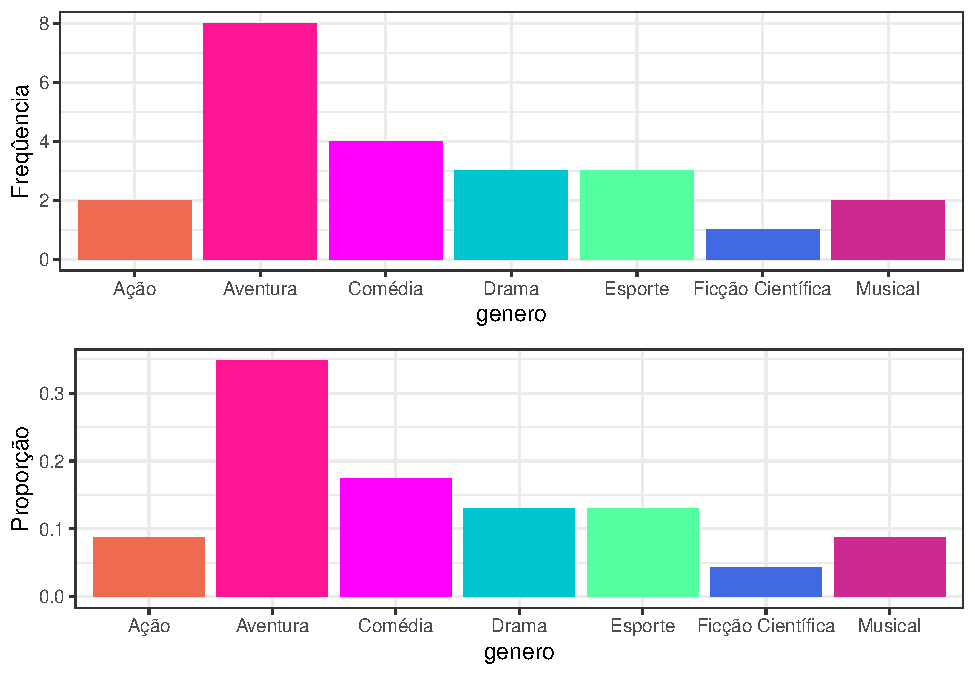
\includegraphics{AED_files/figure-latex/graf_genero-1} \end{center}

\begin{itemize}
\tightlist
\item
  \textbf{Exemplo 2: Variável Quantitativa} (duração do filme)
\end{itemize}

\begin{table}[!h]
\centering\begingroup\fontsize{8}{10}\selectfont

\resizebox{\ifdim\width>\linewidth\linewidth\else\width\fi}{!}{
\begin{tabular}[t]{ccc}
\toprule
\cellcolor[HTML]{D3D3D3}{\textcolor{black}{\textbf{Faixa\_duracao}}} & \cellcolor[HTML]{D3D3D3}{\textcolor{black}{\textbf{Freq}}} & \cellcolor[HTML]{D3D3D3}{\textcolor{black}{\textbf{FreqRel}}}\\
\midrule
\cellcolor{gray!10}{{}[81,86]} & \cellcolor{gray!10}{1} & \cellcolor{gray!10}{0.0434783}\\
(91,96] & 7 & 0.3043478\\
\cellcolor{gray!10}{(96,101]} & \cellcolor{gray!10}{5} & \cellcolor{gray!10}{0.2173913}\\
(101,106] & 6 & 0.2608696\\
\cellcolor{gray!10}{(106,111]} & \cellcolor{gray!10}{1} & \cellcolor{gray!10}{0.0434783}\\
\addlinespace
(111,116] & 1 & 0.0434783\\
\cellcolor{gray!10}{NA} & \cellcolor{gray!10}{2} & \cellcolor{gray!10}{0.0869565}\\
\bottomrule
\end{tabular}}
\endgroup{}
\end{table}

\begin{Shaded}
\begin{Highlighting}[]
\NormalTok{tab\_duracao }\SpecialCharTok{\%\textgreater{}\%} 
  \FunctionTok{ggplot}\NormalTok{() }\SpecialCharTok{+} \FunctionTok{theme\_bw}\NormalTok{() }\SpecialCharTok{+} \FunctionTok{xlab}\NormalTok{(}\StringTok{"Duração do filme"}\NormalTok{) }\SpecialCharTok{+} \FunctionTok{ylab}\NormalTok{(}\StringTok{"Proporção"}\NormalTok{) }\SpecialCharTok{+}
  \FunctionTok{geom\_bar}\NormalTok{(}\FunctionTok{aes}\NormalTok{(}\AttributeTok{x=}\NormalTok{ Faixa\_duracao, }\AttributeTok{y=}\NormalTok{ FreqRel), }\AttributeTok{fill=}\StringTok{"royalblue"}\NormalTok{, }\AttributeTok{stat=}\StringTok{"identity"}\NormalTok{)}
\end{Highlighting}
\end{Shaded}

\begin{center}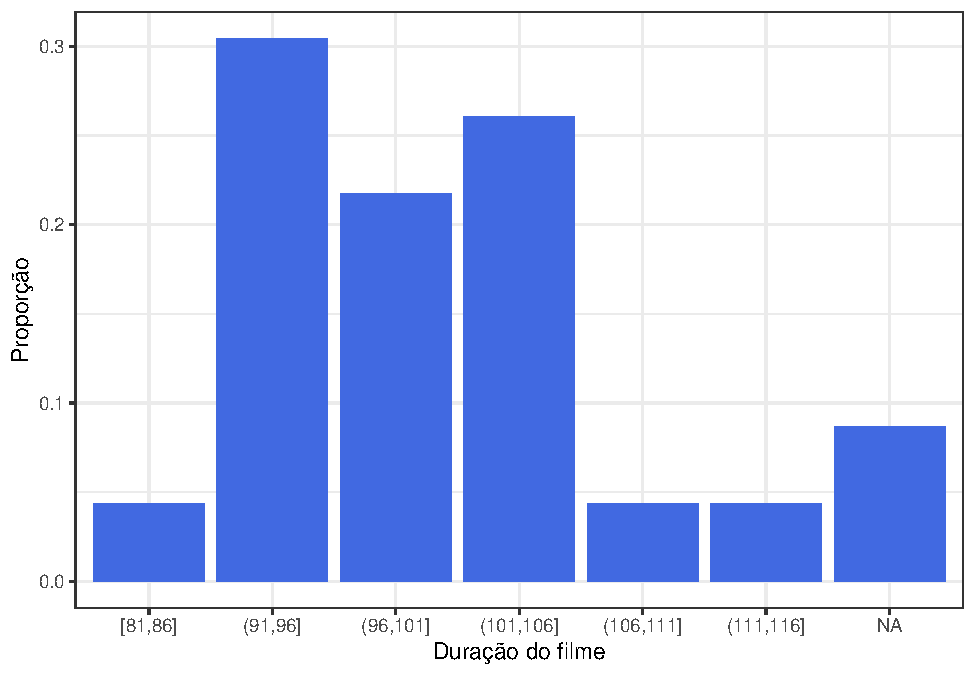
\includegraphics{AED_files/figure-latex/graf_duracao-1} \end{center}

\begin{center}\rule{0.5\linewidth}{0.5pt}\end{center}

\section{Gráfico de Setores (Pizza)}\label{gruxe1fico-de-setores-pizza}

\begin{itemize}
\tightlist
\item
  Pode ser utilizado para variáveis qualitativas.
\end{itemize}

\begin{Shaded}
\begin{Highlighting}[]
\NormalTok{pizza\_genero }\OtherTok{\textless{}{-}}\NormalTok{ tab\_genero }\SpecialCharTok{\%\textgreater{}\%} 
  \FunctionTok{mutate}\NormalTok{(}\AttributeTok{Porc =}\NormalTok{ scales}\SpecialCharTok{::}\FunctionTok{percent}\NormalTok{(FreqRel)) }\SpecialCharTok{\%\textgreater{}\%} 
  \FunctionTok{ggplot}\NormalTok{(}\FunctionTok{aes}\NormalTok{(}\AttributeTok{x =} \StringTok{""}\NormalTok{, }\AttributeTok{y =}\NormalTok{ FreqRel, }\AttributeTok{fill =}\NormalTok{ Gênero)) }\SpecialCharTok{+}
  \FunctionTok{geom\_col}\NormalTok{(}\AttributeTok{color =} \StringTok{"white"}\NormalTok{) }\SpecialCharTok{+} 
  \FunctionTok{geom\_label}\NormalTok{(}\FunctionTok{aes}\NormalTok{(}\AttributeTok{label =}\NormalTok{ Porc), }\CommentTok{\#color = c(1, "white", "white"),}
        \AttributeTok{position =} \FunctionTok{position\_stack}\NormalTok{(}\AttributeTok{vjust =} \FloatTok{0.5}\NormalTok{),}
        \AttributeTok{show.legend =} \ConstantTok{FALSE}\NormalTok{) }\SpecialCharTok{+} \FunctionTok{guides}\NormalTok{(}\AttributeTok{fill =} \FunctionTok{guide\_legend}\NormalTok{(}\AttributeTok{title =} \StringTok{""}\NormalTok{)) }\SpecialCharTok{+}
        \FunctionTok{scale\_fill\_manual}\NormalTok{(}\StringTok{"Gênero dos filmes"}\NormalTok{, }\AttributeTok{values =}\FunctionTok{c}\NormalTok{(}\StringTok{"Aventura"} \OtherTok{=} \StringTok{"deeppink"}\NormalTok{, }
                        \StringTok{"Comédia"} \OtherTok{=} \StringTok{"magenta"}\NormalTok{, }\StringTok{"Ação"} \OtherTok{=} \StringTok{"coral2"}\NormalTok{, }
                        \StringTok{"Esporte"} \OtherTok{=} \StringTok{"seagreen1"}\NormalTok{, }\StringTok{"Drama"} \OtherTok{=} \StringTok{"turquoise3"}\NormalTok{, }
                        \StringTok{"Musical"} \OtherTok{=} \StringTok{"maroon3"}\NormalTok{, }\StringTok{"Ficção Científica"} \OtherTok{=} \StringTok{"royalblue1"}\NormalTok{)) }\SpecialCharTok{+}
  \FunctionTok{coord\_polar}\NormalTok{(}\AttributeTok{theta =} \StringTok{"y"}\NormalTok{) }\SpecialCharTok{+} \FunctionTok{ggtitle}\NormalTok{(}\StringTok{"Gênero dos filmes"}\NormalTok{) }\SpecialCharTok{+}
  \FunctionTok{theme\_void}\NormalTok{() }\SpecialCharTok{+} \FunctionTok{theme}\NormalTok{(}\AttributeTok{legend.position=}\StringTok{"bottom"}\NormalTok{, }
                       \AttributeTok{plot.title =} \FunctionTok{element\_text}\NormalTok{(}\AttributeTok{hjust =} \FloatTok{0.5}\NormalTok{))}

\NormalTok{ggpubr}\SpecialCharTok{::}\FunctionTok{ggarrange}\NormalTok{(pizza\_genero)}
\end{Highlighting}
\end{Shaded}

\begin{center}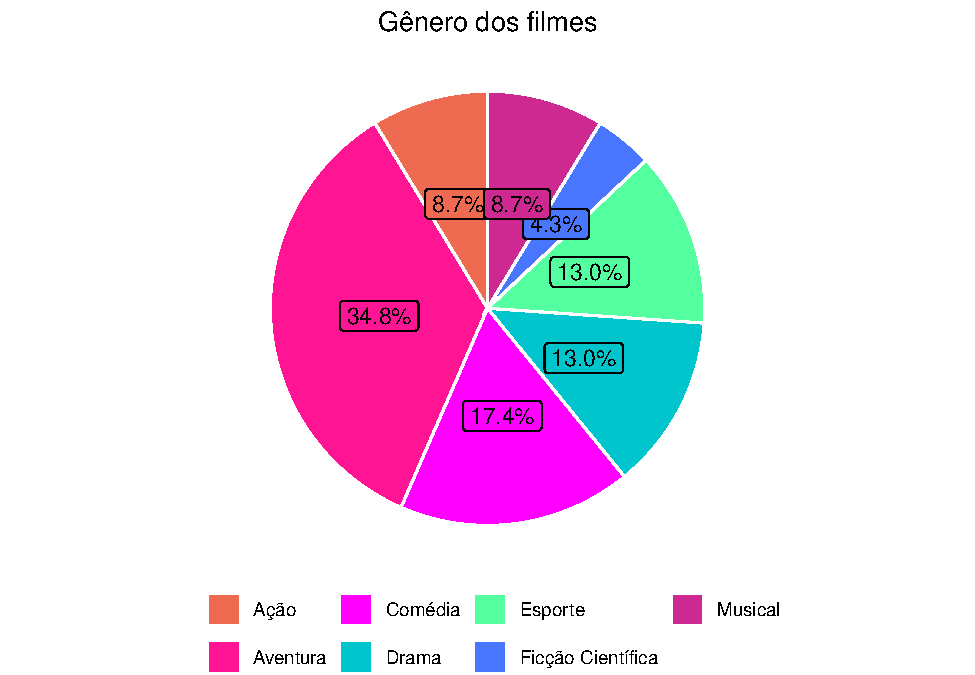
\includegraphics{AED_files/figure-latex/pizza1-1} \end{center}

\begin{itemize}
\tightlist
\item
  Por que deve ser evitado?

  \begin{itemize}
  \tightlist
  \item
    Quando as frequências são muito pequenas (abaixo de 5\%, por exemplo), as fatias se tornam de difícil visualização.\\
  \item
    Dependem do uso de cores. Isso pode dificultar a escolha de cores que sejam suficientemente contrastantes para uma melhor visualização. Isso pode ser ainda mais prejudicado dependendo do dispotitivo que for visualizar o gráfico (se a impressão ou o monitor for de baixa qualidade, por exemplo). Por fim, isso pode dificultar a visualização por pessoas que tem dificuldades em enxergar cores (cerca de 8\% da população masculina é daltônica, por exemplo).\\
  \item
    A comparação direta entre dois gráficos de pizza é bem mais difícil que em gráficos de barras. No segundo é bem mais facil visualizar diferenças, se esse for seu objetivo.\\
  \item
    Ainda assim, podem ser utilizados em casos específicos onde os problemas anteriores não ocorrem (quando há poucas categorias, nenhuma delas com frequencias muito baixas e as diferenças são muito evidentes ou o objetivo não é fazer comparações).
  \end{itemize}
\end{itemize}

\begin{center}\rule{0.5\linewidth}{0.5pt}\end{center}

\section{Histograma}\label{histograma}

\begin{itemize}
\tightlist
\item
  Adequado para variáveis quantitativas (contínuas).\\
\item
  Apesar de ser parecido com o gráfico de barras, no histograma as bases dos retângulos são proporcionais aos intervalos das classes e as áreas de cada retângulo devem ser proporcionais às frequências de cada classe.
\end{itemize}

\begin{table}[!h]
\centering\begingroup\fontsize{8}{10}\selectfont

\resizebox{\ifdim\width>\linewidth\linewidth\else\width\fi}{!}{
\begin{tabular}[t]{ccc}
\toprule
\cellcolor[HTML]{D3D3D3}{\textcolor{black}{\textbf{Bilheteria\_Mundial}}} & \cellcolor[HTML]{D3D3D3}{\textcolor{black}{\textbf{Freq}}} & \cellcolor[HTML]{D3D3D3}{\textcolor{black}{\textbf{FreqRel}}}\\
\midrule
\cellcolor{gray!10}{1.1 bilhão |-- 1.3 bilhão} & \cellcolor{gray!10}{1} & \cellcolor{gray!10}{0.0434783}\\
300 milhões |-- 500 milhões & 8 & 0.3478261\\
\cellcolor{gray!10}{500 milhões |-- 700 milhões} & \cellcolor{gray!10}{6} & \cellcolor{gray!10}{0.2608696}\\
700 milhões |-- 900 milhões & 5 & 0.2173913\\
\cellcolor{gray!10}{900 milhões |-- 1.1 bilhão} & \cellcolor{gray!10}{3} & \cellcolor{gray!10}{0.1304348}\\
\bottomrule
\end{tabular}}
\endgroup{}
\end{table}

\begin{Shaded}
\begin{Highlighting}[]
\NormalTok{filmes\_pixar }\SpecialCharTok{\%\textgreater{}\%} \FunctionTok{ggplot}\NormalTok{() }\SpecialCharTok{+} \FunctionTok{theme\_bw}\NormalTok{() }\SpecialCharTok{+}
  \FunctionTok{geom\_histogram}\NormalTok{(}\FunctionTok{aes}\NormalTok{(bilheteria\_mundial), }\AttributeTok{color=}\StringTok{"black"}\NormalTok{, }\AttributeTok{fill=}\StringTok{"royalblue"}\NormalTok{, }
                 \AttributeTok{breaks=} \FunctionTok{c}\NormalTok{(}\DecValTok{300000000}\NormalTok{, }\DecValTok{500000000}\NormalTok{, }\DecValTok{700000000}\NormalTok{, }\DecValTok{900000000}\NormalTok{, }
                           \DecValTok{1100000000}\NormalTok{, }\DecValTok{1300000000}\NormalTok{))}
\end{Highlighting}
\end{Shaded}

\begin{center}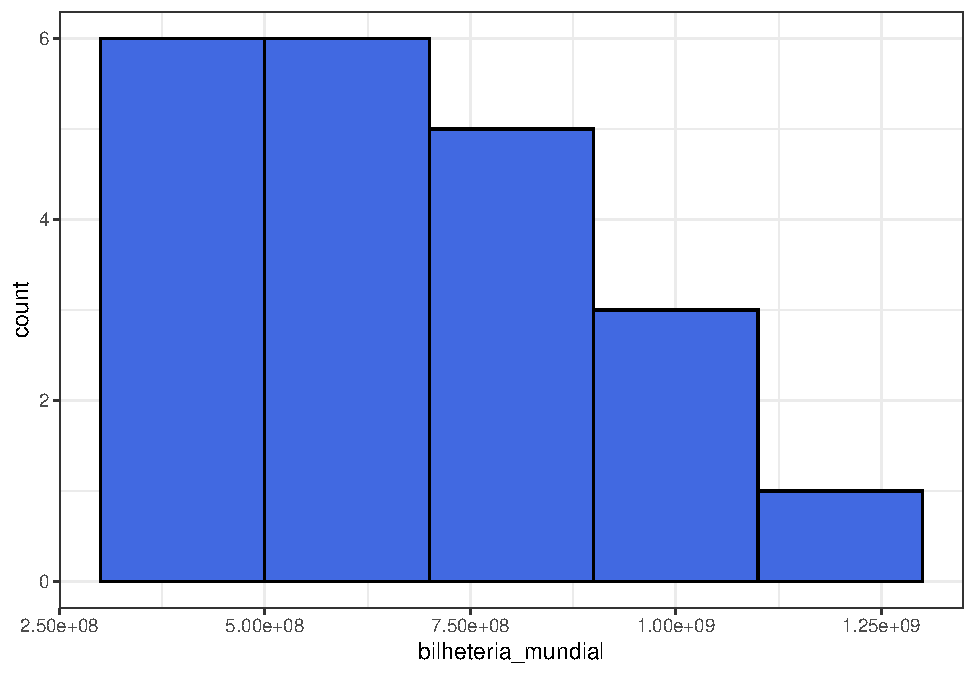
\includegraphics{AED_files/figure-latex/hist_bilheteria1-1} \end{center}

\begin{itemize}
\tightlist
\item
  Quando as faixas tem tamanhos diferentes, não é adequado usar as frequências absolutas ou relativas no eixo y pois a área do gráfico correspondente pode dar a impressão de que as frequências são maiores do que efetivamente foi observado. É possível ver isso no gráfico a seguir.\\
\item
  Neste caso, o ideal é utilizar a \emph{densidade de frequência} no eixo y, dada por \(d_i = \frac{f_i}{\delta_i}\), onde \(\delta_i\) é o comprimento da faixa.
\end{itemize}

\begin{table}[!h]
\centering\begingroup\fontsize{8}{10}\selectfont

\resizebox{\ifdim\width>\linewidth\linewidth\else\width\fi}{!}{
\begin{tabular}[t]{ccccc}
\toprule
\cellcolor[HTML]{D3D3D3}{\textcolor{black}{\textbf{Bilheteria\_Mundial}}} & \cellcolor[HTML]{D3D3D3}{\textcolor{black}{\textbf{Freq}}} & \cellcolor[HTML]{D3D3D3}{\textcolor{black}{\textbf{FreqRel}}} & \cellcolor[HTML]{D3D3D3}{\textcolor{black}{\textbf{delta}}} & \cellcolor[HTML]{D3D3D3}{\textcolor{black}{\textbf{Dens}}}\\
\midrule
\cellcolor{gray!10}{1.1 bilhão |-- 1.3 bilhão} & \cellcolor{gray!10}{1} & \cellcolor{gray!10}{0.0434783} & \cellcolor{gray!10}{0.2} & \cellcolor{gray!10}{0.2173913}\\
300 milhões |-- 500 milhões & 8 & 0.3478261 & 0.1 & 3.4782609\\
\cellcolor{gray!10}{500 milhões |-- 700 milhões} & \cellcolor{gray!10}{6} & \cellcolor{gray!10}{0.2608696} & \cellcolor{gray!10}{0.1} & \cellcolor{gray!10}{2.6086957}\\
700 milhões |-- 900 milhões & 5 & 0.2173913 & 0.1 & 2.1739130\\
\cellcolor{gray!10}{900 milhões |-- 1.1 bilhão} & \cellcolor{gray!10}{3} & \cellcolor{gray!10}{0.1304348} & \cellcolor{gray!10}{0.1} & \cellcolor{gray!10}{1.3043478}\\
\bottomrule
\end{tabular}}
\endgroup{}
\end{table}

\begin{Shaded}
\begin{Highlighting}[]
\CommentTok{\#hist\_bilheteria\_c \textless{}{-} }
\NormalTok{filmes\_pixar }\SpecialCharTok{\%\textgreater{}\%} \FunctionTok{ggplot}\NormalTok{() }\SpecialCharTok{+} \FunctionTok{theme\_bw}\NormalTok{() }\SpecialCharTok{+}
  \FunctionTok{geom\_histogram}\NormalTok{(}\FunctionTok{aes}\NormalTok{(bilheteria\_mundial), }\AttributeTok{color=}\StringTok{"black"}\NormalTok{, }\AttributeTok{fill=}\StringTok{"royalblue"}\NormalTok{, }
                 \AttributeTok{breaks=} \FunctionTok{c}\NormalTok{(}\DecValTok{300000000}\NormalTok{, }\DecValTok{500000000}\NormalTok{, }\DecValTok{700000000}\NormalTok{, }\DecValTok{900000000}\NormalTok{, }
                           \DecValTok{1100000000}\NormalTok{, }\DecValTok{1300000000}\NormalTok{))}
\end{Highlighting}
\end{Shaded}

\begin{center}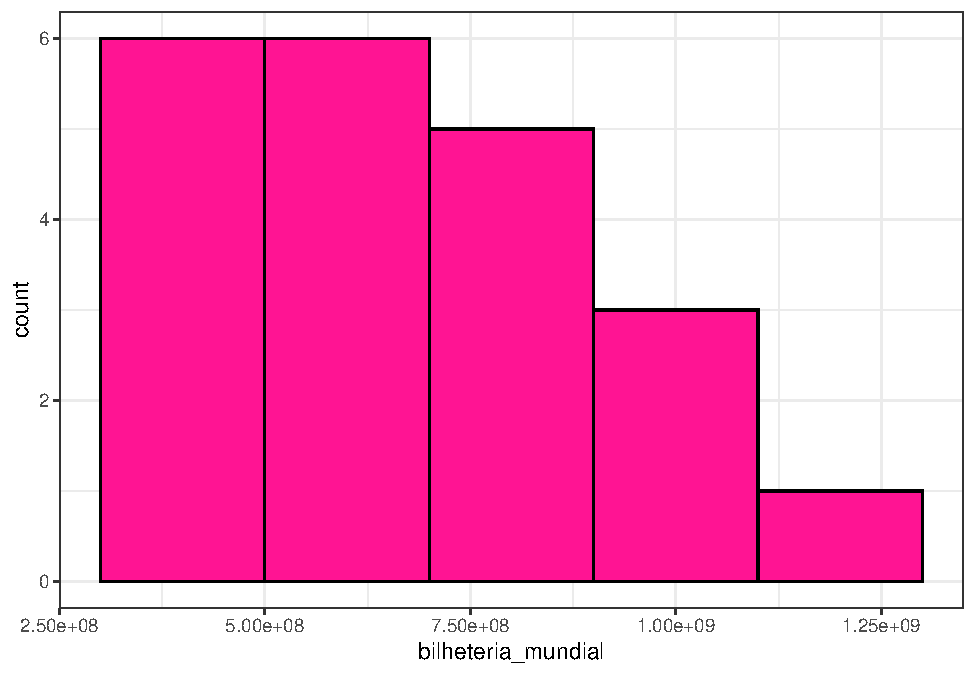
\includegraphics{AED_files/figure-latex/hist_bilheteria2-1} \end{center}

\begin{Shaded}
\begin{Highlighting}[]
\CommentTok{\#hist\_bilheteria\_m \textless{}{-} }
\NormalTok{filmes\_pixar }\SpecialCharTok{\%\textgreater{}\%} \FunctionTok{ggplot}\NormalTok{() }\SpecialCharTok{+} \FunctionTok{theme\_bw}\NormalTok{() }\SpecialCharTok{+}
  \FunctionTok{geom\_histogram}\NormalTok{(}\FunctionTok{aes}\NormalTok{(bilheteria\_mundial,}\FunctionTok{after\_stat}\NormalTok{(density)), }
                 \AttributeTok{color=}\StringTok{"black"}\NormalTok{, }\AttributeTok{fill=}\StringTok{"royalblue"}\NormalTok{, }
                 \AttributeTok{breaks=} \FunctionTok{c}\NormalTok{(}\DecValTok{300000000}\NormalTok{, }\DecValTok{500000000}\NormalTok{, }\DecValTok{700000000}\NormalTok{, }\DecValTok{900000000}\NormalTok{, }
                           \DecValTok{1100000000}\NormalTok{, }\DecValTok{1300000000}\NormalTok{))}
\end{Highlighting}
\end{Shaded}

\begin{center}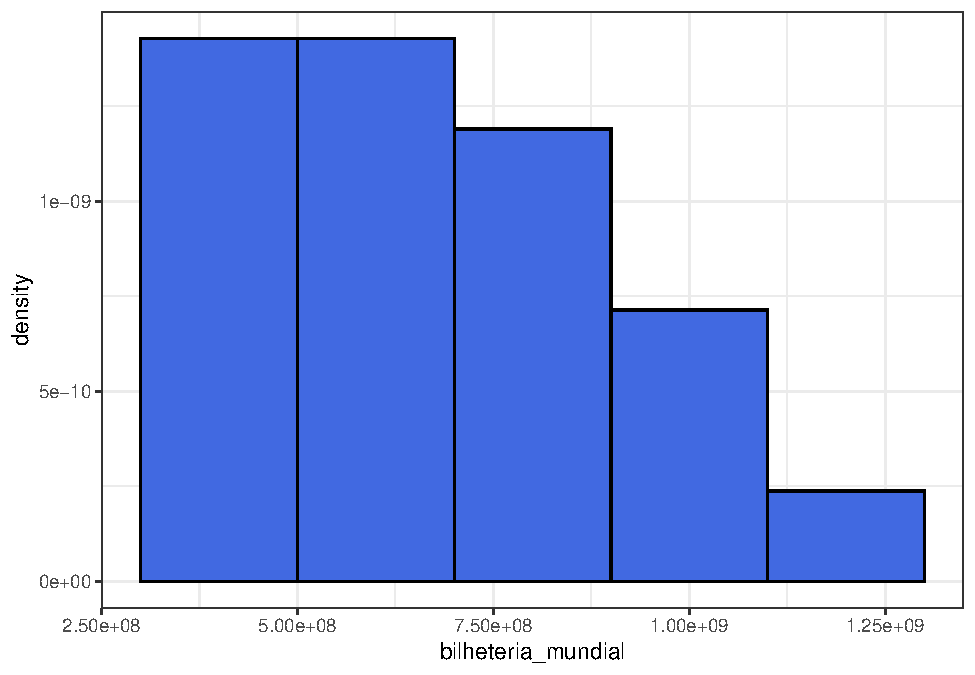
\includegraphics{AED_files/figure-latex/hist_bilheteria2-2} \end{center}

\begin{Shaded}
\begin{Highlighting}[]
\CommentTok{\#ggpubr::ggarrange(hist\_bilheteria\_c, hist\_bilheteria\_m, ncol=1)}
\end{Highlighting}
\end{Shaded}

\begin{itemize}
\tightlist
\item
  Note que desta forma, a área total do histograma é igual a 1.
\end{itemize}

\subsection{Números de faixas e largura}\label{nuxfameros-de-faixas-e-largura}

Para construir um histograma, não existe um número correto de faixas, e diferentes larguras podem revelar diferentes aspectos dos dados. Faixas mais largas ajudam a reduzir o ruído onde há poucos dados, enquanto faixas mais estreitas aumentam a precisão onde há muitos dados. Existem diferentes métodos para fazer essa escolha, alguns exemplos são:

\textbf{Fórmula de Sturges:}

Uma opção simples é usar a \emph{Fórmula de Sturges}, que calcula o número de faixas a partir do tamanho da amostra:

\[
k = \lceil \log_2 n \rceil + 1
\]
Esse é o método padrão usado pelo R base. Como esse método calcula o número de faixas com base no tamanho da amostra \(n\), ela pode ter um desempenho ruim quando \(n < 30\), pois gera poucas faixas, o que dificulta a visualização de tendências. Para grandes conjunto de dados, ela pode superestimar a largura das faixas, gerando um histogramas execivamente suavizado. Além disso, pode não funcionar bem para dados que não seguem uma distribuição simétrica.

\textbf{Regra de Referência Normal de Scoot:}

Outra método é a \emph{Regra de Referência Normal de Scott}, que busca minimizar o erro na estimativa da densidade. Ela define a largura \(h\) das faixas como:

\[
h = \frac{3,49 \cdot \text{desvio padrão}}{\sqrt[3]{n}}
\]

Essa abordagem é melhor para dados com variabilidade semelhante à de uma distribuição simétrica.

\textbf{Regra de Freedman-Diaconis:}

Outro exemplo é a regra de Freedman--Diaconis, que é mais robusta a dados assimétricos ou com outliers, usando o intervalo interquartil (IQR) no lugar do desvio padrão, ele define a largura \(h\) das faixas como:

\[
h = 2 \cdot \frac{\text{IQR}(x)}{\sqrt[3]{n}}
\]

Ela se adapta melhor a distribuições que não são tão bem comportadas.

\textbf{Exemplo no R:}

Para criar um histograma no R usando o número de faixas (ou largura das faixas) usando a fórmula desejada, é possível calcular o valor manualmente e depois passá-lo para o argumento breaks da função \emph{hist()}.

\begin{Shaded}
\begin{Highlighting}[]
\CommentTok{\# Exemplo usando a fórmula de Sturges:}
\NormalTok{n }\OtherTok{\textless{}{-}} \FunctionTok{length}\NormalTok{(dados)  }\CommentTok{\# Tamanho da amostra}
\NormalTok{k\_sturges }\OtherTok{\textless{}{-}} \DecValTok{1} \SpecialCharTok{+} \FunctionTok{log2}\NormalTok{(n)  }\CommentTok{\# Fórmula de Sturges}

\FunctionTok{hist}\NormalTok{(dados, }\AttributeTok{breaks =}\NormalTok{ k\_sturges)}
\end{Highlighting}
\end{Shaded}

Além disso, também é possível usar um número de faixas diretamente, colocando o valor de breaks como um número inteiro.

Assim, dependendo do tipo de dado e do objetivo da análise, podemos escolher o método mais adequado para definir o número de faixas no histograma. Para encontrar outros métodos e fórmulas, basta acessar o site \textbf{\href{https://en.wikipedia.org/wiki/Histogram\#Number_of_bins_and_width}{aqui}}.

\begin{center}\rule{0.5\linewidth}{0.5pt}\end{center}

\section{Ramos e Folhas}\label{ramos-e-folhas}

\begin{itemize}
\tightlist
\item
  Similar a um histograma mas com menos perda de informação.
\end{itemize}

\begin{table}[!h]
\centering\begingroup\fontsize{8}{10}\selectfont

\resizebox{\ifdim\width>\linewidth\linewidth\else\width\fi}{!}{
\begin{tabular}[t]{c}
\toprule
\cellcolor[HTML]{D3D3D3}{\textcolor{black}{\textbf{duracao}}}\\
\midrule
\cellcolor{gray!10}{81}\\
\cellcolor{gray!10}{92}\\
92\\
\cellcolor{gray!10}{93}\\
93\\
\addlinespace
\cellcolor{gray!10}{95}\\
95\\
96\\
\cellcolor{gray!10}{97}\\
98\\
\addlinespace
\cellcolor{gray!10}{\cellcolor{gray!10}{100}}\\
100\\
100\\
\cellcolor{gray!10}{102}\\
102\\
\addlinespace
103\\
\cellcolor{gray!10}{104}\\
105\\
\cellcolor{gray!10}{106}\\
111\\
\addlinespace
\cellcolor{gray!10}{115}\\
117\\
\cellcolor{gray!10}{118}\\
\bottomrule
\end{tabular}}
\endgroup{}
\end{table}

\begin{Shaded}
\begin{Highlighting}[]
\FunctionTok{stem}\NormalTok{(filmes\_pixar}\SpecialCharTok{$}\NormalTok{duracao)}
\end{Highlighting}
\end{Shaded}

\begin{verbatim}
## 
##   The decimal point is 1 digit(s) to the right of the |
## 
##    8 | 1
##    9 | 223355678
##   10 | 000223456
##   11 | 1578
\end{verbatim}

\begin{table}[!h]
\centering\begingroup\fontsize{8}{10}\selectfont

\resizebox{\ifdim\width>\linewidth\linewidth\else\width\fi}{!}{
\begin{tabular}[t]{ccccc}
\toprule
\cellcolor[HTML]{D3D3D3}{\textcolor{black}{\textbf{Bilheteria\_Mundial}}} & \cellcolor[HTML]{D3D3D3}{\textcolor{black}{\textbf{Freq}}} & \cellcolor[HTML]{D3D3D3}{\textcolor{black}{\textbf{FreqRel}}} & \cellcolor[HTML]{D3D3D3}{\textcolor{black}{\textbf{delta}}} & \cellcolor[HTML]{D3D3D3}{\textcolor{black}{\textbf{Dens}}}\\
\midrule
\cellcolor{gray!10}{1.1 bilhão |-- 1.3 bilhão} & \cellcolor{gray!10}{1} & \cellcolor{gray!10}{0.0434783} & \cellcolor{gray!10}{0.1} & \cellcolor{gray!10}{0.4347826}\\
300 milhões |-- 500 milhões & 8 & 0.3478261 & 0.1 & 3.4782609\\
\cellcolor{gray!10}{500 milhões |-- 700 milhões} & \cellcolor{gray!10}{6} & \cellcolor{gray!10}{0.2608696} & \cellcolor{gray!10}{0.1} & \cellcolor{gray!10}{2.6086957}\\
700 milhões |-- 900 milhões & 5 & 0.2173913 & 0.1 & 2.1739130\\
\cellcolor{gray!10}{900 milhões |-- 1.1 bilhão} & \cellcolor{gray!10}{3} & \cellcolor{gray!10}{0.1304348} & \cellcolor{gray!10}{0.1} & \cellcolor{gray!10}{1.3043478}\\
\bottomrule
\end{tabular}}
\endgroup{}
\end{table}

\begin{Shaded}
\begin{Highlighting}[]
\FunctionTok{stem}\NormalTok{(filmes\_pixar}\SpecialCharTok{$}\NormalTok{bilheteria\_mundial }\SpecialCharTok{/} \FloatTok{1e9}\NormalTok{) }
\end{Highlighting}
\end{Shaded}

\begin{verbatim}
## 
##   The decimal point is at the |
## 
##   0 | 113444
##   0 | 5555666677899
##   1 | 0112
\end{verbatim}

\begin{itemize}
\tightlist
\item
  Não é adequado quando temos grandes bancos de dados e não tem o mesmo efeito visual de um boxplot.
\end{itemize}

\begin{center}\rule{0.5\linewidth}{0.5pt}\end{center}

\section{Box-Plot}\label{box-plot}

\begin{itemize}
\tightlist
\item
  Utilizado para representar graficamente os quartis, além dos valores mínimo e máximo.
\end{itemize}

\begin{Shaded}
\begin{Highlighting}[]
\NormalTok{filmes\_pixar }\SpecialCharTok{\%\textgreater{}\%} \FunctionTok{ggplot}\NormalTok{() }\SpecialCharTok{+} \FunctionTok{theme\_bw}\NormalTok{() }\SpecialCharTok{+} 
  \FunctionTok{geom\_boxplot}\NormalTok{(}\FunctionTok{aes}\NormalTok{(}\AttributeTok{y=}\NormalTok{duracao), }\AttributeTok{color=}\StringTok{"black"}\NormalTok{, }\AttributeTok{fill=}\StringTok{"royalblue"}\NormalTok{) }
\end{Highlighting}
\end{Shaded}

\begin{center}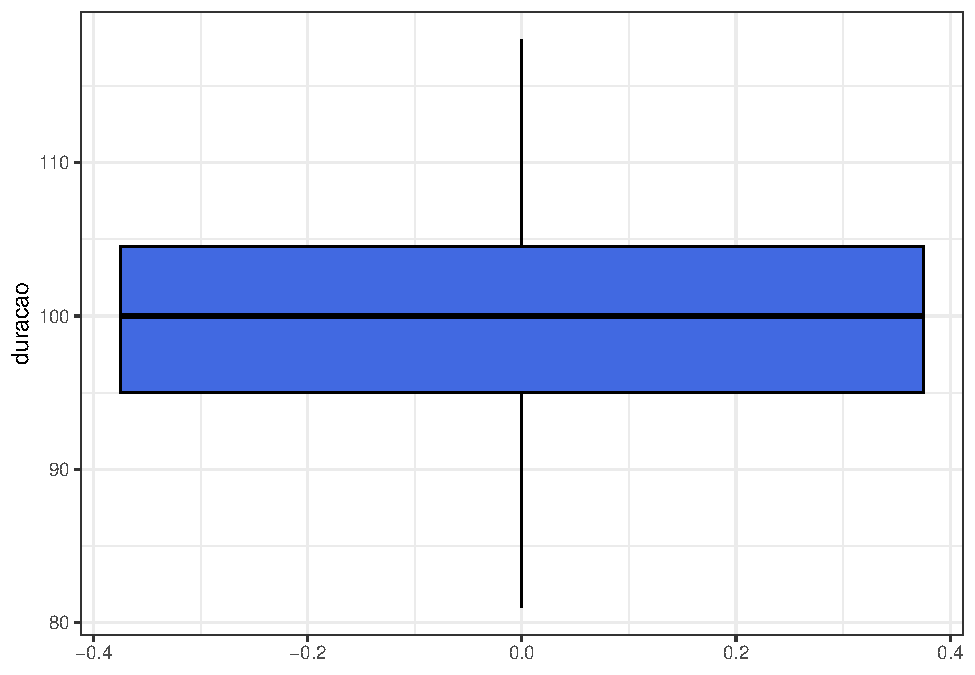
\includegraphics{AED_files/figure-latex/boxplot_duracao-1} \end{center}

\begin{itemize}
\item
  No retângulo estão representados os quartis \(q_1\), \(q_2\) e \(q_3\).\\
\item
  A reta acima do retângulo se estende até o valor máximo observado, desde que esse não seja maior que \(q_3 + 1.5 \cdot d_q\).\\
\item
  Do mesmo modo, a reta abaixo do retângulo do retângulo se estende até o mínimo, desde que esse não seja menor que \(q_1 - 1.5 \cdot d_q\).\\
\item
  Se houver valores que excedam os limites acima propostos, a reta acima (abaixo) do retângulo vai até o maior (menor) valor menor (maior) que \(q_3 + 1.5 \cdot d_q\) \(\left(q_1 - 1.5 \cdot d_q\right)\).\\
\item
  Os valores fora destes limites serão representados por asteriscos e são chamados de \emph{outliers} (ou \emph{valores atípicos})
\item
  É possivel incluir os pontos observados no boxplot para não ter perda de informação.
\end{itemize}

\begin{Shaded}
\begin{Highlighting}[]
\NormalTok{filmes\_pixar }\SpecialCharTok{\%\textgreater{}\%} \FunctionTok{ggplot}\NormalTok{(}\FunctionTok{aes}\NormalTok{(}\AttributeTok{x=}\StringTok{""}\NormalTok{,}\AttributeTok{y=}\NormalTok{duracao)) }\SpecialCharTok{+} \FunctionTok{theme\_bw}\NormalTok{() }\SpecialCharTok{+} 
  \FunctionTok{geom\_boxplot}\NormalTok{(}\AttributeTok{color=}\StringTok{"black"}\NormalTok{, }\AttributeTok{fill=}\StringTok{"royalblue"}\NormalTok{) }\SpecialCharTok{+} 
\NormalTok{  ggbeeswarm}\SpecialCharTok{::}\FunctionTok{geom\_beeswarm}\NormalTok{(}\AttributeTok{cex=}\DecValTok{3}\NormalTok{,}\AttributeTok{size=}\DecValTok{3}\NormalTok{,}\AttributeTok{method =} \StringTok{"center"}\NormalTok{)}
\end{Highlighting}
\end{Shaded}

\begin{center}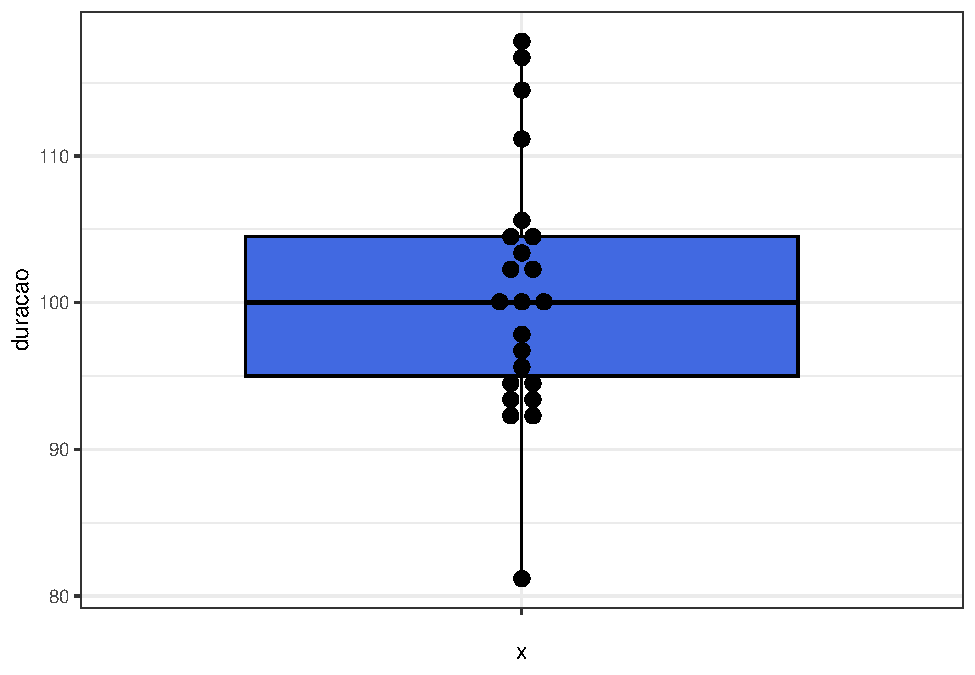
\includegraphics{AED_files/figure-latex/boxplot_P_duracao-1} \end{center}

\begin{Shaded}
\begin{Highlighting}[]
  \CommentTok{\#geom\_dotplot(binaxis= "y",stackdir = "center",fill = 1,dotsize = 0.8,stackratio=2)}
  \CommentTok{\#geom\_jitter(color="black", size=1, alpha=0.9)}
\end{Highlighting}
\end{Shaded}

\begin{center}\rule{0.5\linewidth}{0.5pt}\end{center}

\section{Gráficos e simetria}\label{gruxe1ficos-e-simetria}

\begin{Shaded}
\begin{Highlighting}[]
\FunctionTok{set.seed}\NormalTok{(}\DecValTok{13}\NormalTok{)}

\NormalTok{simul }\OtherTok{\textless{}{-}} \FunctionTok{tibble}\NormalTok{(}\AttributeTok{y =} \FunctionTok{rnorm}\NormalTok{(}\DecValTok{150}\NormalTok{,}\FloatTok{2.5}\NormalTok{,}\DecValTok{1}\NormalTok{))}
\NormalTok{lim }\OtherTok{=} \FunctionTok{c}\NormalTok{(}\FunctionTok{min}\NormalTok{(simul}\SpecialCharTok{$}\NormalTok{y),}\FunctionTok{max}\NormalTok{(simul}\SpecialCharTok{$}\NormalTok{y))}

\NormalTok{hist }\OtherTok{\textless{}{-}}\NormalTok{ simul }\SpecialCharTok{\%\textgreater{}\%} \FunctionTok{ggplot}\NormalTok{() }\SpecialCharTok{+} \FunctionTok{theme\_classic}\NormalTok{() }\SpecialCharTok{+} \FunctionTok{xlab}\NormalTok{(}\StringTok{""}\NormalTok{) }\SpecialCharTok{+} \FunctionTok{xlim}\NormalTok{(lim[}\DecValTok{1}\NormalTok{],lim[}\DecValTok{2}\NormalTok{]) }\SpecialCharTok{+} 
  \FunctionTok{ggtitle}\NormalTok{(}\StringTok{"Simetria"}\NormalTok{) }\SpecialCharTok{+}
  \FunctionTok{geom\_histogram}\NormalTok{(}\FunctionTok{aes}\NormalTok{(y,}\FunctionTok{after\_stat}\NormalTok{(density)), }
                 \AttributeTok{color=}\StringTok{"black"}\NormalTok{, }\AttributeTok{fill=}\StringTok{"royalblue"}\NormalTok{, }\AttributeTok{bins=}\DecValTok{8}\NormalTok{)}

\NormalTok{box }\OtherTok{\textless{}{-}}\NormalTok{ simul }\SpecialCharTok{\%\textgreater{}\%} \FunctionTok{ggplot}\NormalTok{(}\FunctionTok{aes}\NormalTok{(}\AttributeTok{x=}\StringTok{""}\NormalTok{,}\AttributeTok{y=}\NormalTok{y)) }\SpecialCharTok{+} 
  \FunctionTok{theme\_classic}\NormalTok{() }\SpecialCharTok{+} \FunctionTok{coord\_flip}\NormalTok{() }\SpecialCharTok{+} \FunctionTok{xlab}\NormalTok{(}\StringTok{""}\NormalTok{) }\SpecialCharTok{+} \FunctionTok{ylab}\NormalTok{(}\StringTok{""}\NormalTok{) }\SpecialCharTok{+} \FunctionTok{ylim}\NormalTok{(lim[}\DecValTok{1}\NormalTok{],lim[}\DecValTok{2}\NormalTok{]) }\SpecialCharTok{+}
  \FunctionTok{geom\_boxplot}\NormalTok{(}\AttributeTok{color=}\StringTok{"black"}\NormalTok{, }\AttributeTok{fill=}\StringTok{"royalblue"}\NormalTok{)  }
  \CommentTok{\#ggbeeswarm::geom\_beeswarm(cex=1,size=1,method = "center")}

\NormalTok{ggpubr}\SpecialCharTok{::}\FunctionTok{ggarrange}\NormalTok{(hist, box, }\AttributeTok{heights =} \FunctionTok{c}\NormalTok{(}\DecValTok{2}\NormalTok{, }\DecValTok{1}\NormalTok{), }\AttributeTok{nrow=}\DecValTok{2}\NormalTok{, }\AttributeTok{align =} \StringTok{"v"}\NormalTok{)}
\end{Highlighting}
\end{Shaded}

\begin{center}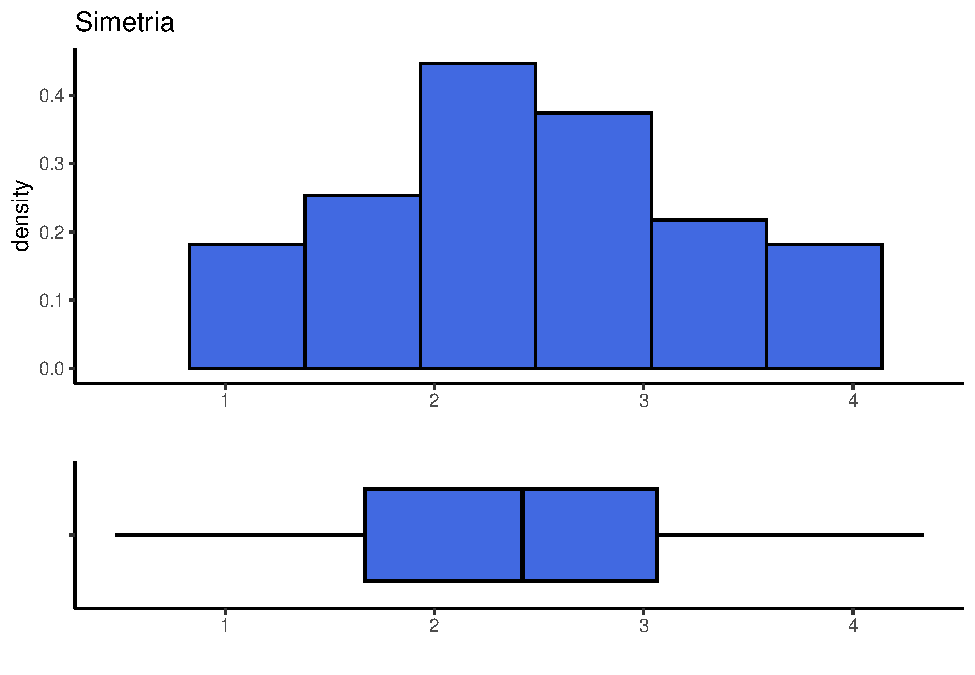
\includegraphics{AED_files/figure-latex/simetria-1} \end{center}

\begin{Shaded}
\begin{Highlighting}[]
\FunctionTok{set.seed}\NormalTok{(}\DecValTok{13}\NormalTok{)}

\NormalTok{simul }\OtherTok{\textless{}{-}} \FunctionTok{tibble}\NormalTok{(}\AttributeTok{y =} \FunctionTok{rgamma}\NormalTok{(}\DecValTok{150}\NormalTok{,}\FloatTok{2.5}\NormalTok{,}\DecValTok{1}\NormalTok{))}
\NormalTok{lim }\OtherTok{=} \FunctionTok{c}\NormalTok{(}\FunctionTok{min}\NormalTok{(simul}\SpecialCharTok{$}\NormalTok{y),}\FunctionTok{max}\NormalTok{(simul}\SpecialCharTok{$}\NormalTok{y))}

\NormalTok{hist }\OtherTok{\textless{}{-}}\NormalTok{ simul }\SpecialCharTok{\%\textgreater{}\%} \FunctionTok{ggplot}\NormalTok{() }\SpecialCharTok{+} \FunctionTok{theme\_classic}\NormalTok{() }\SpecialCharTok{+} \FunctionTok{xlab}\NormalTok{(}\StringTok{""}\NormalTok{) }\SpecialCharTok{+} \FunctionTok{xlim}\NormalTok{(lim[}\DecValTok{1}\NormalTok{],lim[}\DecValTok{2}\NormalTok{]) }\SpecialCharTok{+}
  \FunctionTok{ggtitle}\NormalTok{(}\StringTok{"Assimetria à Direita"}\NormalTok{) }\SpecialCharTok{+}
  \FunctionTok{geom\_histogram}\NormalTok{(}\FunctionTok{aes}\NormalTok{(y,}\FunctionTok{after\_stat}\NormalTok{(density)), }
                 \AttributeTok{color=}\StringTok{"black"}\NormalTok{, }\AttributeTok{fill=}\StringTok{"royalblue"}\NormalTok{, }\AttributeTok{bins=}\DecValTok{10}\NormalTok{)}

\NormalTok{box }\OtherTok{\textless{}{-}}\NormalTok{ simul }\SpecialCharTok{\%\textgreater{}\%} \FunctionTok{ggplot}\NormalTok{(}\FunctionTok{aes}\NormalTok{(}\AttributeTok{x=}\StringTok{""}\NormalTok{,}\AttributeTok{y=}\NormalTok{y)) }\SpecialCharTok{+} 
  \FunctionTok{theme\_classic}\NormalTok{() }\SpecialCharTok{+} \FunctionTok{coord\_flip}\NormalTok{() }\SpecialCharTok{+} \FunctionTok{xlab}\NormalTok{(}\StringTok{""}\NormalTok{) }\SpecialCharTok{+} \FunctionTok{ylab}\NormalTok{(}\StringTok{""}\NormalTok{) }\SpecialCharTok{+} \FunctionTok{ylim}\NormalTok{(lim[}\DecValTok{1}\NormalTok{],lim[}\DecValTok{2}\NormalTok{]) }\SpecialCharTok{+}
  \FunctionTok{geom\_boxplot}\NormalTok{(}\AttributeTok{color=}\StringTok{"black"}\NormalTok{, }\AttributeTok{fill=}\StringTok{"royalblue"}\NormalTok{)  }
  \CommentTok{\#ggbeeswarm::geom\_beeswarm(cex=1,size=1,method = "center")}

\NormalTok{ggpubr}\SpecialCharTok{::}\FunctionTok{ggarrange}\NormalTok{(hist, box, }\AttributeTok{heights =} \FunctionTok{c}\NormalTok{(}\DecValTok{2}\NormalTok{, }\DecValTok{1}\NormalTok{), }\AttributeTok{nrow=}\DecValTok{2}\NormalTok{, }\AttributeTok{align =} \StringTok{"v"}\NormalTok{)}
\end{Highlighting}
\end{Shaded}

\begin{center}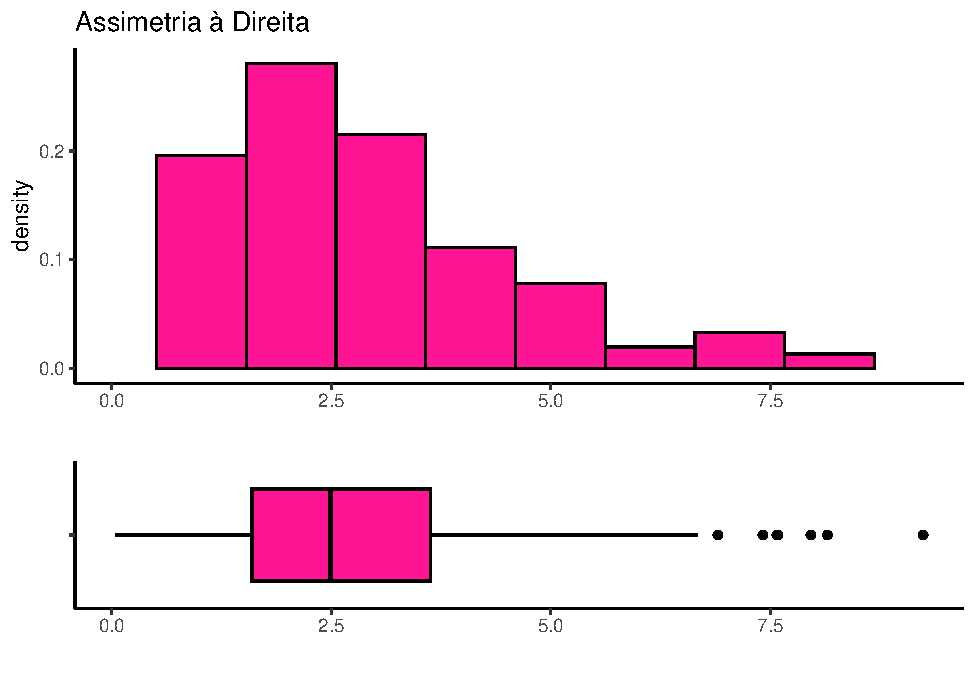
\includegraphics{AED_files/figure-latex/assimetriaD-1} \end{center}

\begin{Shaded}
\begin{Highlighting}[]
\NormalTok{simul }\OtherTok{\textless{}{-}}\NormalTok{ lim[}\DecValTok{2}\NormalTok{]}\SpecialCharTok{{-}}\NormalTok{simul}\SpecialCharTok{+}\NormalTok{lim[}\DecValTok{1}\NormalTok{]}
\NormalTok{lim }\OtherTok{=} \FunctionTok{c}\NormalTok{(}\FunctionTok{min}\NormalTok{(simul}\SpecialCharTok{$}\NormalTok{y),}\FunctionTok{max}\NormalTok{(simul}\SpecialCharTok{$}\NormalTok{y))}

\NormalTok{hist }\OtherTok{\textless{}{-}}\NormalTok{ simul }\SpecialCharTok{\%\textgreater{}\%} \FunctionTok{ggplot}\NormalTok{() }\SpecialCharTok{+} \FunctionTok{theme\_classic}\NormalTok{() }\SpecialCharTok{+} \FunctionTok{xlab}\NormalTok{(}\StringTok{""}\NormalTok{) }\SpecialCharTok{+} \FunctionTok{xlim}\NormalTok{(lim[}\DecValTok{1}\NormalTok{],lim[}\DecValTok{2}\NormalTok{]) }\SpecialCharTok{+}
  \FunctionTok{ggtitle}\NormalTok{(}\StringTok{"Assimetria à Esquerda"}\NormalTok{) }\SpecialCharTok{+}
  \FunctionTok{geom\_histogram}\NormalTok{(}\FunctionTok{aes}\NormalTok{(y,}\FunctionTok{after\_stat}\NormalTok{(density)), }
                 \AttributeTok{color=}\StringTok{"black"}\NormalTok{, }\AttributeTok{fill=}\StringTok{"royalblue"}\NormalTok{, }\AttributeTok{bins=}\DecValTok{10}\NormalTok{)}

\NormalTok{box }\OtherTok{\textless{}{-}}\NormalTok{ simul }\SpecialCharTok{\%\textgreater{}\%} \FunctionTok{ggplot}\NormalTok{(}\FunctionTok{aes}\NormalTok{(}\AttributeTok{x=}\StringTok{""}\NormalTok{,}\AttributeTok{y=}\NormalTok{y)) }\SpecialCharTok{+} 
  \FunctionTok{theme\_classic}\NormalTok{() }\SpecialCharTok{+} \FunctionTok{coord\_flip}\NormalTok{() }\SpecialCharTok{+} \FunctionTok{xlab}\NormalTok{(}\StringTok{""}\NormalTok{) }\SpecialCharTok{+} \FunctionTok{ylab}\NormalTok{(}\StringTok{""}\NormalTok{) }\SpecialCharTok{+} \FunctionTok{ylim}\NormalTok{(lim[}\DecValTok{1}\NormalTok{],lim[}\DecValTok{2}\NormalTok{]) }\SpecialCharTok{+}
  \FunctionTok{geom\_boxplot}\NormalTok{(}\AttributeTok{color=}\StringTok{"black"}\NormalTok{, }\AttributeTok{fill=}\StringTok{"royalblue"}\NormalTok{)  }
  \CommentTok{\#ggbeeswarm::geom\_beeswarm(cex=1,size=1,method = "center")}

\NormalTok{ggpubr}\SpecialCharTok{::}\FunctionTok{ggarrange}\NormalTok{(hist, box, }\AttributeTok{heights =} \FunctionTok{c}\NormalTok{(}\DecValTok{2}\NormalTok{, }\DecValTok{1}\NormalTok{), }\AttributeTok{nrow=}\DecValTok{2}\NormalTok{, }\AttributeTok{align =} \StringTok{"v"}\NormalTok{)}
\end{Highlighting}
\end{Shaded}

\begin{center}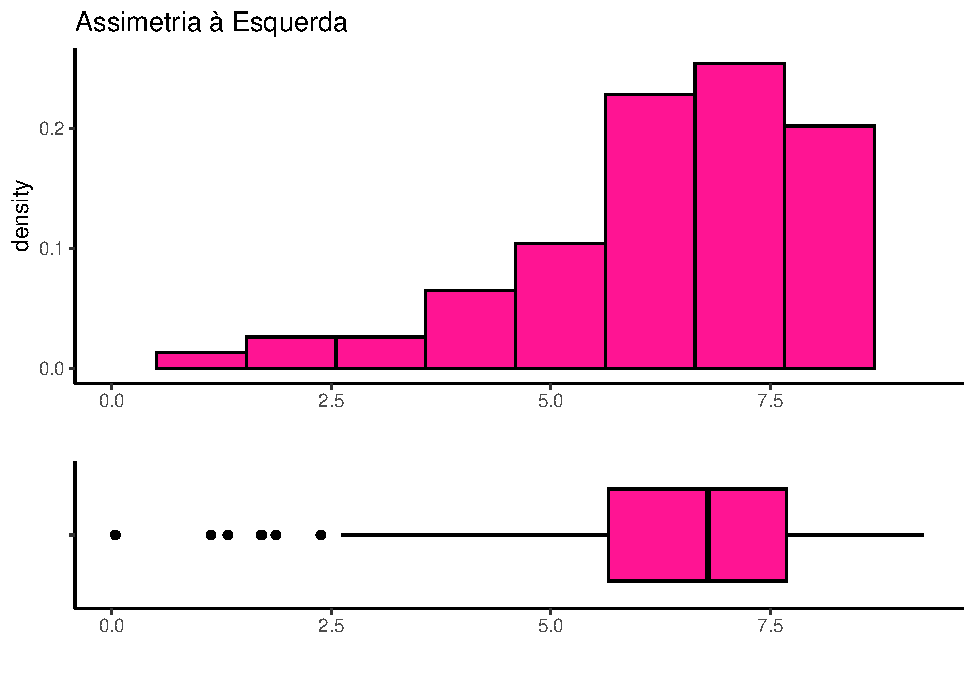
\includegraphics{AED_files/figure-latex/assimetriaE-1} \end{center}

\begin{itemize}
\item
  Os quartis são medidas de posição que auxiliam na avaliação da simetria dos dados. Para uma distribuição aproximadamente \textbf{simétrica}, espera-se que

  \begin{itemize}
  \tightlist
  \item
    \(q_2 - x(1) ~\approx~ x(n)-q_2\) ,\\
  \item
    \(q_2 - q_1 ~\approx~ q_3-q_2\) ,\\
  \item
    \(q_1 - x(1) ~\approx~ x(n)-q_3\) .
  \end{itemize}
\item
  A distribiuição dos dados é dita \textbf{assimétrica à direita} se as diferenças entre os quantis situados a direita da mediana e a mediana são maiores que as diferenças entre a mediana e os quantis situados à esquerda da mediana. Se o contrário ocorre, dizemos que a distribuição é \textbf{assimétrica à esquerda}.
\item
  Além disso, se uma distribuição é aproximadamente simétrica,

  \begin{itemize}
  \tightlist
  \item
    \(q_2-x_{(i)} ~\approx~ x_{(n+1-i)}-q_2\) , \(i=1,\ldots,\lfloor(n+1)/2\rfloor\) , em que \(\lfloor y \rfloor\) é o maior inteiro menor ou igual a \(y\).
  \end{itemize}
\item
  Assim, defina \(u_i = q_2-x_{(i)}\) e \(v_i = x_{(n+1-i)}-q_2\), para \(i=1,\ldots,\lfloor(n+1)/2\rfloor\). Então,

  \begin{itemize}
  \tightlist
  \item
    Se a distribuição é simetrica, espera-se que \(u_i \approx v_i\) ;
  \item
    Se a distribuição é assimetrica à direira, espera-se que \(u_i \leq v_i\) ;
  \item
    Se a distribuição é assimetrica à esquerda, espera-se que \(u_i \geq v_i\).
  \end{itemize}
\item
  Uma forma de fazer essa avaliação é fazer um gráfico dos pares \((u_i,v_i)\).
\end{itemize}

\begin{Shaded}
\begin{Highlighting}[]
\FunctionTok{tibble}\NormalTok{(}\AttributeTok{u =} \FloatTok{100.6522} \SpecialCharTok{{-}} \FunctionTok{sort}\NormalTok{(filmes\_pixar}\SpecialCharTok{$}\NormalTok{duracao)[}\DecValTok{1}\SpecialCharTok{:}\DecValTok{5}\NormalTok{],}
       \AttributeTok{v =} \FunctionTok{sort}\NormalTok{(filmes\_pixar}\SpecialCharTok{$}\NormalTok{duracao,}\AttributeTok{decreasing=}\ConstantTok{TRUE}\NormalTok{)[}\DecValTok{1}\SpecialCharTok{:}\DecValTok{5}\NormalTok{] }\SpecialCharTok{{-}} \FloatTok{100.6522}\NormalTok{) }\SpecialCharTok{\%\textgreater{}\%} 
  \FunctionTok{ggplot}\NormalTok{() }\SpecialCharTok{+} \FunctionTok{theme\_bw}\NormalTok{() }\SpecialCharTok{+} 
  \FunctionTok{geom\_point}\NormalTok{(}\FunctionTok{aes}\NormalTok{(}\AttributeTok{x=}\NormalTok{u,}\AttributeTok{y=}\NormalTok{v)) }\SpecialCharTok{+} 
  \FunctionTok{geom\_line}\NormalTok{(}\FunctionTok{aes}\NormalTok{(}\AttributeTok{x=}\NormalTok{u,}\AttributeTok{y=}\NormalTok{u))}
\end{Highlighting}
\end{Shaded}

\begin{center}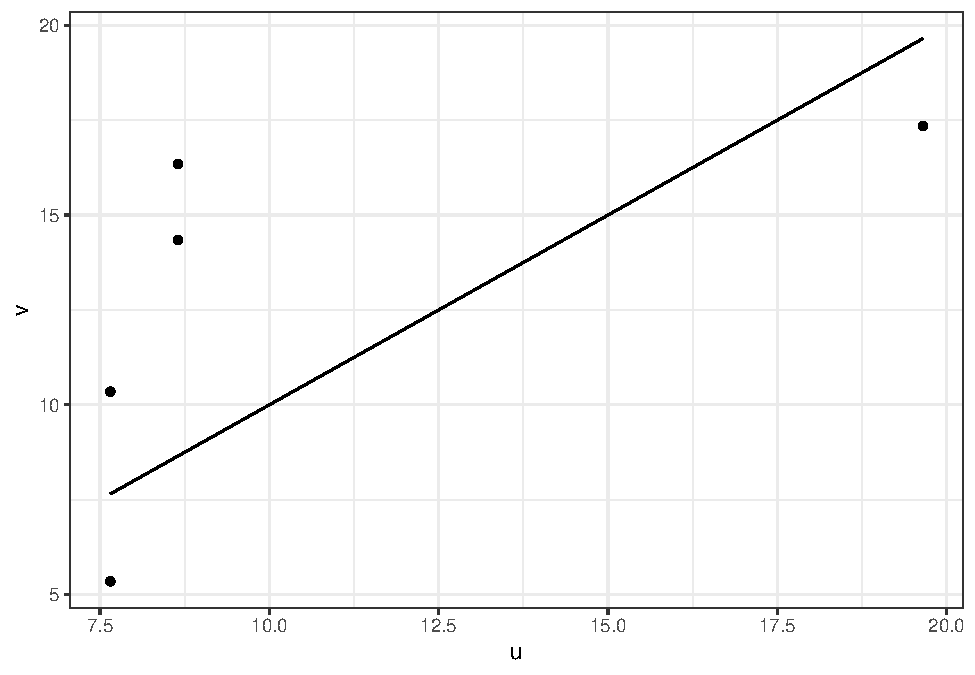
\includegraphics{AED_files/figure-latex/graf_simetria-1} \end{center}

\begin{center}\rule{0.5\linewidth}{0.5pt}\end{center}

\section{Exercícios}\label{exercuxedcios-1}

\begin{enumerate}
\def\labelenumi{\arabic{enumi}.}
\tightlist
\item
  Escolha um banco de dados de sua preferência no R ou na internet contendo pelo menos duas variáveis quantitativas (preferencialmente contínuas). Crie um arquivo de RMarkdown e faça:
\end{enumerate}

\begin{enumerate}
\def\labelenumi{\alph{enumi}.}
\tightlist
\item
  um histograma
\item
  um boxplot
\end{enumerate}

\begin{center}\rule{0.5\linewidth}{0.5pt}\end{center}

\chapter{Análise bivariada}\label{anaise_bi7}

\begin{itemize}
\item
  Considere que o interesse agora é estudar a relação entre variáveis. Se não há associação entre duas ou mais variáveis, dizemos que elas são independentes.
\item
  \textbf{Exemplo:} suponha que deseja-se estudar se a cor da roupa (1: clara, 0: escura) está associado com gostar de basquete (1: sim, 0: não). Perguntei para 10 alunos da turma e os dados estão apresentados abaixo
\end{itemize}

\begin{Shaded}
\begin{Highlighting}[]
\NormalTok{dados\_cap7 }\OtherTok{\textless{}{-}} \FunctionTok{tibble}\NormalTok{(}\AttributeTok{Camisa=}\FunctionTok{c}\NormalTok{(}\DecValTok{1}\NormalTok{,}\DecValTok{1}\NormalTok{,}\DecValTok{1}\NormalTok{,}\DecValTok{1}\NormalTok{,}\DecValTok{1}\NormalTok{,}\DecValTok{0}\NormalTok{,}\DecValTok{0}\NormalTok{,}\DecValTok{0}\NormalTok{,}\DecValTok{0}\NormalTok{,}\DecValTok{0}\NormalTok{),}
                \AttributeTok{Basquete=}\FunctionTok{c}\NormalTok{(}\DecValTok{1}\NormalTok{,}\DecValTok{0}\NormalTok{,}\DecValTok{1}\NormalTok{,}\DecValTok{0}\NormalTok{,}\DecValTok{1}\NormalTok{,}\DecValTok{0}\NormalTok{,}\DecValTok{0}\NormalTok{,}\DecValTok{0}\NormalTok{,}\DecValTok{1}\NormalTok{,}\DecValTok{0}\NormalTok{))}
\end{Highlighting}
\end{Shaded}

\section{Duas variáveis categóricas}\label{duas-variuxe1veis-categuxf3ricas}

\textbf{Tabela de Contingência (de Frequências)}

\begin{itemize}
\tightlist
\item
  Para variáveis categóricas, vamos primeiramente considerar tabelas de frequências.
\end{itemize}

\begin{Shaded}
\begin{Highlighting}[]
\CommentTok{\# R base}
\NormalTok{tab1 }\OtherTok{\textless{}{-}} \FunctionTok{table}\NormalTok{(dados\_cap7}\SpecialCharTok{$}\NormalTok{Camisa,dados\_cap7}\SpecialCharTok{$}\NormalTok{Basquete)}
\NormalTok{tab1}
\end{Highlighting}
\end{Shaded}

\begin{verbatim}
##    
##     0 1
##   0 4 1
##   1 2 3
\end{verbatim}

\begin{itemize}
\item
  Lembre-se que podemos pensam em independência com relação à distribuição conjunta ou à distribuição condicional.
\item
  Se o objetivo é estudar a distribuição conjunta, podemos considerar as frequências relativas ao tamanho total da amostra observada.
\end{itemize}

\begin{Shaded}
\begin{Highlighting}[]
\CommentTok{\# Tidyverse}
\FunctionTok{require}\NormalTok{(gtsummary)}
\end{Highlighting}
\end{Shaded}

\begin{verbatim}
## Carregando pacotes exigidos: gtsummary
\end{verbatim}

\begin{Shaded}
\begin{Highlighting}[]
\NormalTok{dados\_cap7 }\SpecialCharTok{\%\textgreater{}\%} \FunctionTok{tbl\_cross}\NormalTok{(Camisa,Basquete,}\AttributeTok{percent =} \StringTok{"cell"}\NormalTok{) }\SpecialCharTok{\%\textgreater{}\%} 
  \FunctionTok{bold\_labels}\NormalTok{()}
\end{Highlighting}
\end{Shaded}

\begin{table}[t]
\fontsize{12.0pt}{14.4pt}\selectfont
\begin{tabular*}{\linewidth}{@{\extracolsep{\fill}}lccc}
\toprule
 & \multicolumn{2}{c}{\textbf{Basquete}} &  \\ 
\cmidrule(lr){2-3}
 & 0 & 1 & \textbf{Total} \\ 
\midrule\addlinespace[2.5pt]
{\bfseries Camisa} &  &  &  \\ 
    0 & 4 (40\%) & 1 (10\%) & 5 (50\%) \\ 
    1 & 2 (20\%) & 3 (30\%) & 5 (50\%) \\ 
{\bfseries Total} & 6 (60\%) & 4 (40\%) & 10 (100\%) \\ 
\bottomrule
\end{tabular*}
\end{table}

\begin{itemize}
\tightlist
\item
  Se o objetivo é estudar a distribuição condicional, podemos considerar as frequências relativas ao total das linhas ou das colunas. Pelo desenho de nosso estudo, eu fixei o total de cada cor da camisa, então a tabela abaixo é construída com relação ao total das linhas.
\end{itemize}

\begin{Shaded}
\begin{Highlighting}[]
\CommentTok{\# Tidyverse com porcentagens das linhas}
\NormalTok{dados\_cap7 }\SpecialCharTok{\%\textgreater{}\%} \FunctionTok{tbl\_cross}\NormalTok{(Camisa,Basquete,}\AttributeTok{percent =} \StringTok{"row"}\NormalTok{) }\SpecialCharTok{\%\textgreater{}\%} 
  \FunctionTok{bold\_labels}\NormalTok{()}
\end{Highlighting}
\end{Shaded}

\begin{table}[t]
\fontsize{12.0pt}{14.4pt}\selectfont
\begin{tabular*}{\linewidth}{@{\extracolsep{\fill}}lccc}
\toprule
 & \multicolumn{2}{c}{\textbf{Basquete}} &  \\ 
\cmidrule(lr){2-3}
 & 0 & 1 & \textbf{Total} \\ 
\midrule\addlinespace[2.5pt]
{\bfseries Camisa} &  &  &  \\ 
    0 & 4 (80\%) & 1 (20\%) & 5 (100\%) \\ 
    1 & 2 (40\%) & 3 (60\%) & 5 (100\%) \\ 
{\bfseries Total} & 6 (60\%) & 4 (40\%) & 10 (100\%) \\ 
\bottomrule
\end{tabular*}
\end{table}

\textbf{Correlação amostral}

\begin{itemize}
\item
  Podemos estimar a \(E[xY]\) como \(\displaystyle \frac{1}{n}\sum_{i=1}^n x_i~y_i\).
\item
  Assim, a \(COV(X,Y)\) pode ser estimada por \(\displaystyle cov = \frac{1}{n}\sum_{i=1}^n x_i~y_i - \bar{x}~\bar{y}\).
\item
  Analogamente, a correção amostral é \[cor = \dfrac{cov}{\sqrt{var(x)var(y)}} = \dfrac{\displaystyle \sum_{i=1}^n x_i~y_i - n~\bar{x}~\bar{y}}{\displaystyle \sqrt{\sum_{i=1}^n (x_i-\bar{x})^2\sum_{j=1}^n(y_j-\bar{y})^2}}~.\]
\item
  No exemplo:
\end{itemize}

\begin{Shaded}
\begin{Highlighting}[]
\FunctionTok{cor}\NormalTok{(dados\_cap7}\SpecialCharTok{$}\NormalTok{Camisa,dados\_cap7}\SpecialCharTok{$}\NormalTok{Basquete)}
\end{Highlighting}
\end{Shaded}

\begin{verbatim}
## [1] 0.4082483
\end{verbatim}

\textbf{Qui-Quadrado de Pearson}

\begin{itemize}
\item
  Sejam \(o_{ij}\) as frequências observadas na \emph{i}-ésima linha e \emph{j}-ésima coluna da tabela, \(o_{i.}\) o total observado na linha \emph{i} e \(o_{.j}\) o total observado na coluna \emph{j}. Sob a hipótese de independência, espera que o valor observado em cada casela da tabela seja \(\displaystyle e_{ij} = \frac{o_{i.}~o_{.j}}{n}\).
\item
  A estatística de Qui-Quadrado é dada por:
  \[Q^2 = \sum_i \sum_j \frac{(o_{ij}-e_{ij})^2}{e_{ij}}~.\]
\item
  No exemplo:
\end{itemize}

\begin{Shaded}
\begin{Highlighting}[]
\NormalTok{chi2 }\OtherTok{=} \FunctionTok{chisq.test}\NormalTok{(tab1)}\SpecialCharTok{$}\NormalTok{statistic}
\NormalTok{chi2}
\end{Highlighting}
\end{Shaded}

\begin{verbatim}
## X-squared 
## 0.4166667
\end{verbatim}

\begin{center}\rule{0.5\linewidth}{0.5pt}\end{center}

\chapter{Medidas de duas variáveis}\label{medidas_duas_va}

\section{Tabela de Contingência (de Frequências)}\label{tabela-de-continguxeancia-de-frequuxeancias}

\begin{itemize}
\tightlist
\item
  Para variáveis categóricas, vamos primeiramente considerar tabelas de frequências.
\end{itemize}

\begin{Shaded}
\begin{Highlighting}[]
\CommentTok{\# R base}
\NormalTok{tab1 }\OtherTok{\textless{}{-}} \FunctionTok{table}\NormalTok{(dados\_cap7}\SpecialCharTok{$}\NormalTok{Camisa,dados\_cap7}\SpecialCharTok{$}\NormalTok{Basquete)}
\NormalTok{tab1}
\end{Highlighting}
\end{Shaded}

\begin{verbatim}
##    
##     0 1
##   0 4 1
##   1 2 3
\end{verbatim}

\begin{itemize}
\item
  Lembre-se que podemos pensam em independência com relação à distribuição conjunta ou à distribuição condicional.
\item
  Se o objetivo é estudar a distribuição conjunta, podemos considerar as frequências relativas ao tamanho total da amostra observada.
\end{itemize}

\begin{Shaded}
\begin{Highlighting}[]
\CommentTok{\# Tidyverse}
\FunctionTok{require}\NormalTok{(gtsummary)}
\NormalTok{dados\_cap7 }\SpecialCharTok{\%\textgreater{}\%} \FunctionTok{tbl\_cross}\NormalTok{(Camisa,Basquete,}\AttributeTok{percent =} \StringTok{"cell"}\NormalTok{) }\SpecialCharTok{\%\textgreater{}\%} 
  \FunctionTok{bold\_labels}\NormalTok{()}
\end{Highlighting}
\end{Shaded}

\begin{table}[t]
\fontsize{12.0pt}{14.4pt}\selectfont
\begin{tabular*}{\linewidth}{@{\extracolsep{\fill}}lccc}
\toprule
 & \multicolumn{2}{c}{\textbf{Basquete}} &  \\ 
\cmidrule(lr){2-3}
 & 0 & 1 & \textbf{Total} \\ 
\midrule\addlinespace[2.5pt]
{\bfseries Camisa} &  &  &  \\ 
    0 & 4 (40\%) & 1 (10\%) & 5 (50\%) \\ 
    1 & 2 (20\%) & 3 (30\%) & 5 (50\%) \\ 
{\bfseries Total} & 6 (60\%) & 4 (40\%) & 10 (100\%) \\ 
\bottomrule
\end{tabular*}
\end{table}

\begin{itemize}
\tightlist
\item
  Se o objetivo é estudar a distribuição condicional, podemos considerar as frequências relativas ao total das linhas ou das colunas. Pelo desenho de nosso estudo, eu fixei o total de cada cor da camisa, então a tabela abaixo é construída com relação ao total das linhas.
\end{itemize}

\begin{Shaded}
\begin{Highlighting}[]
\CommentTok{\# Tidyverse com porcentagens das linhas}
\NormalTok{dados\_cap7 }\SpecialCharTok{\%\textgreater{}\%} \FunctionTok{tbl\_cross}\NormalTok{(Camisa,Basquete,}\AttributeTok{percent =} \StringTok{"row"}\NormalTok{) }\SpecialCharTok{\%\textgreater{}\%} 
  \FunctionTok{bold\_labels}\NormalTok{()}
\end{Highlighting}
\end{Shaded}

\begin{table}[t]
\fontsize{12.0pt}{14.4pt}\selectfont
\begin{tabular*}{\linewidth}{@{\extracolsep{\fill}}lccc}
\toprule
 & \multicolumn{2}{c}{\textbf{Basquete}} &  \\ 
\cmidrule(lr){2-3}
 & 0 & 1 & \textbf{Total} \\ 
\midrule\addlinespace[2.5pt]
{\bfseries Camisa} &  &  &  \\ 
    0 & 4 (80\%) & 1 (20\%) & 5 (100\%) \\ 
    1 & 2 (40\%) & 3 (60\%) & 5 (100\%) \\ 
{\bfseries Total} & 6 (60\%) & 4 (40\%) & 10 (100\%) \\ 
\bottomrule
\end{tabular*}
\end{table}

\section{Correlação amostral}\label{correlauxe7uxe3o-amostral}

\begin{itemize}
\item
  Podemos estimar a \(E[xY]\) como \(\displaystyle \frac{1}{n}\sum_{i=1}^n x_i~y_i\).
\item
  Assim, a \(COV(X,Y)\) pode ser estimada por \(\displaystyle cov = \frac{1}{n}\sum_{i=1}^n x_i~y_i - \bar{x}~\bar{y}\).
\item
  Analogamente, a correção amostral é \[cor = \dfrac{cov}{\sqrt{var(x)var(y)}} = \dfrac{\displaystyle \sum_{i=1}^n x_i~y_i - n~\bar{x}~\bar{y}}{\displaystyle \sqrt{\sum_{i=1}^n (x_i-\bar{x})^2\sum_{j=1}^n(y_j-\bar{y})^2}}~.\]
\item
  No exemplo:
\end{itemize}

\begin{Shaded}
\begin{Highlighting}[]
\FunctionTok{cor}\NormalTok{(dados\_cap7}\SpecialCharTok{$}\NormalTok{Camisa, dados\_cap7}\SpecialCharTok{$}\NormalTok{Basquete)}
\end{Highlighting}
\end{Shaded}

\begin{verbatim}
## [1] 0.4082483
\end{verbatim}

\section{Qui-Quadrado de Pearson}\label{qui-quadrado-de-pearson}

\begin{itemize}
\item
  Sejam \(o_{ij}\) as frequências observadas na \emph{i}-ésima linha e \emph{j}-ésima coluna da tabela, \(o_{i.}\) o total observado na linha \emph{i} e \(o_{.j}\) o total observado na coluna \emph{j}. Sob a hipótese de independência, espera que o valor observado em cada casela da tabela seja \(\displaystyle e_{ij} = \frac{o_{i.}~o_{.j}}{n}\).
\item
  A estatística de Qui-Quadrado é dada por:
  \[Q^2 = \sum_i \sum_j \frac{(o_{ij}-e_{ij})^2}{e_{ij}}~.\]
\item
  No exemplo:
\end{itemize}

\begin{Shaded}
\begin{Highlighting}[]
\NormalTok{chi2 }\OtherTok{=} \FunctionTok{chisq.test}\NormalTok{(tab1)}\SpecialCharTok{$}\NormalTok{statistic}
\NormalTok{chi2}
\end{Highlighting}
\end{Shaded}

\begin{verbatim}
## X-squared 
## 0.4166667
\end{verbatim}

\begin{center}\rule{0.5\linewidth}{0.5pt}\end{center}

\section{Medidas de Associação baseadas no Qui-Quadrado}\label{medidas-de-associauxe7uxe3o-baseadas-no-qui-quadrado}

\begin{Shaded}
\begin{Highlighting}[]
\FunctionTok{require}\NormalTok{(gtsummary)}
\NormalTok{dados\_cap7 }\SpecialCharTok{\%\textgreater{}\%} \FunctionTok{tbl\_cross}\NormalTok{(Camisa, Basquete, }\AttributeTok{percent =} \StringTok{"cell"}\NormalTok{) }\SpecialCharTok{\%\textgreater{}\%}
  \FunctionTok{bold\_labels}\NormalTok{()}
\end{Highlighting}
\end{Shaded}

\begin{table}[t]
\fontsize{12.0pt}{14.4pt}\selectfont
\begin{tabular*}{\linewidth}{@{\extracolsep{\fill}}lccc}
\toprule
 & \multicolumn{2}{c}{\textbf{Basquete}} &  \\ 
\cmidrule(lr){2-3}
 & 0 & 1 & \textbf{Total} \\ 
\midrule\addlinespace[2.5pt]
{\bfseries Camisa} &  &  &  \\ 
    0 & 4 (40\%) & 1 (10\%) & 5 (50\%) \\ 
    1 & 2 (20\%) & 3 (30\%) & 5 (50\%) \\ 
{\bfseries Total} & 6 (60\%) & 4 (40\%) & 10 (100\%) \\ 
\bottomrule
\end{tabular*}
\end{table}

\subsection{Coeficiente de Contingência de Pearson}\label{coeficiente-de-continguxeancia-de-pearson}

\[C = \sqrt{\frac{Q^2}{Q^2 + n}} \qquad 0\leq C\leq1\]

No exemplo:\\
\[C = \sqrt{\frac{\frac{10}{6}}{\frac{10}{6} + 10}} = 0.791\]

O Coeficiente de Contingência de Pearson é muito influenciado pelo número de linhas (\(l\)) e número de colunas (\(c\)).

\subsection{Coeficiente de Tcschupov}\label{coeficiente-de-tcschupov}

\[T = \sqrt{\frac{Q^2/n}{(l - 1) (c - 1)}} \qquad 0\leq T\leq1\]

No exemplo:

\[T = \sqrt{\frac{\frac{1.66}{10}}{(2 - 1) (2 - 1)}} = 0.41\]

\begin{center}\rule{0.5\linewidth}{0.5pt}\end{center}

\section{Outras Medidas de Associação}\label{outras-medidas-de-associauxe7uxe3o}

\begin{itemize}
\tightlist
\item
  Considere um contexto em que deseja-se avalia a presença de um desfecho (ter um determinado cancer, gostar de basquete, etc) na presença de um fator de risco (fumar, usar roupa clara).
\end{itemize}

\begin{Shaded}
\begin{Highlighting}[]
\FunctionTok{require}\NormalTok{(kableExtra)}
\FunctionTok{tibble}\NormalTok{(}\StringTok{\textquotesingle{}Fator de Risco\textquotesingle{}} \OtherTok{=} \FunctionTok{c}\NormalTok{(}\StringTok{"Não"}\NormalTok{, }\StringTok{"Sim"}\NormalTok{), }
       \StringTok{\textquotesingle{}Sem o Desfecho\textquotesingle{}} \OtherTok{=} \FunctionTok{c}\NormalTok{(}\StringTok{"(1{-}q)"}\NormalTok{, }\StringTok{"(1{-}p)"}\NormalTok{), }
       \StringTok{\textquotesingle{}Com o Desfecho\textquotesingle{}} \OtherTok{=} \FunctionTok{c}\NormalTok{(}\StringTok{"q"}\NormalTok{, }\StringTok{"p"}\NormalTok{)) }\SpecialCharTok{\%\textgreater{}\%} 
  \FunctionTok{kbl}\NormalTok{(}\AttributeTok{align =} \StringTok{\textquotesingle{}c\textquotesingle{}}\NormalTok{, }\AttributeTok{format =} \StringTok{"html"}\NormalTok{, }\AttributeTok{booktabs =} \ConstantTok{TRUE}\NormalTok{)}\SpecialCharTok{\%\textgreater{}\%} 
  \FunctionTok{kable\_styling}\NormalTok{(}
     \AttributeTok{bootstrap\_options =} \FunctionTok{c}\NormalTok{(}\StringTok{"striped"}\NormalTok{,}\StringTok{"hover"}\NormalTok{, }\StringTok{"bordered"}\NormalTok{, }\StringTok{"condensed"}\NormalTok{), }
     \AttributeTok{latex\_options =} \FunctionTok{c}\NormalTok{(}\StringTok{"striped"}\NormalTok{))}
\end{Highlighting}
\end{Shaded}

Fator de Risco

Sem o Desfecho

Com o Desfecho

Não

(1-q)

q

Sim

(1-p)

p

\subsection{Risco Atribuível}\label{risco-atribuuxedvel}

\begin{itemize}
\tightlist
\item
  \(RA = p - q\): é a diferença entre as probabilidades de ter a doença dado a presença do fator de risco e de ter a doença sem fator de risco.\\
\item
  No exemplo:
\end{itemize}

\[RA =    \frac{3}{5} - {1 \over 5} = \frac{2}{5}\]

\subsection{Risco Relativo}\label{risco-relativo}

\begin{itemize}
\tightlist
\item
  \(RR = p/q\): é quantas vezes é mais provavél ter a doença tendo o fator de risco em relação a quem não tem.\\
\item
  No exemplo:
\end{itemize}

\[RR = \frac{3/5}{1/5} = 3  \]

\subsection{Razão de Chances (``Odds Ratio'')}\label{razuxe3o-de-chances-odds-ratio}

\begin{itemize}
\tightlist
\item
  Os termos probabilidade e chance são sinônimos mas, por convenção, usaremos a notação \(3:2  ~``="~ \dfrac{3}{5}\), sendo que \(3:2 = \dfrac{3/5}{2/5}\) denotará a chance e \(\dfrac{3}{5}\) a probabilidade.
\end{itemize}

\[OR ~=~ \frac{p}{(1-p)} \div \frac{q}{(1-q)} ~=~  \frac{p(1-q)}{q(1-q)}\]\\
- No exemplo:

\[OR ~=~ \frac{3/5}{2/5} \div \frac{1/5}{4/5} ~=~ \frac{3}{2} \div {1 \over 4} ~=~ \frac{3}{2} ~.~  \frac{4}{1} =  6\]

\begin{center}\rule{0.5\linewidth}{0.5pt}\end{center}

\section{Medidas para Testes de Diagnóstico}\label{medidas-para-testes-de-diagnuxf3stico}

Considere um teste para uma determinada doença, de modo que o resultado do teste pode ser 1: \emph{Positivo} e 0: \emph{Negativo} e o indivíduos podem estar 1: \emph{Doente} ou 0: \emph{Não Doente}.

\begin{Shaded}
\begin{Highlighting}[]
\FunctionTok{require}\NormalTok{(gtsummary)}

\NormalTok{dados }\OtherTok{\textless{}{-}} \FunctionTok{tibble}\NormalTok{(}\AttributeTok{Teste =} \FunctionTok{c}\NormalTok{(}\DecValTok{1}\NormalTok{,}\DecValTok{1}\NormalTok{,}\DecValTok{1}\NormalTok{,}\DecValTok{1}\NormalTok{,}\DecValTok{1}\NormalTok{,}\DecValTok{0}\NormalTok{,}\DecValTok{0}\NormalTok{,}\DecValTok{0}\NormalTok{,}\DecValTok{0}\NormalTok{,}\DecValTok{0}\NormalTok{),}
                \AttributeTok{Doente =} \FunctionTok{c}\NormalTok{(}\DecValTok{1}\NormalTok{,}\DecValTok{0}\NormalTok{,}\DecValTok{1}\NormalTok{,}\DecValTok{0}\NormalTok{,}\DecValTok{1}\NormalTok{,}\DecValTok{0}\NormalTok{,}\DecValTok{0}\NormalTok{,}\DecValTok{0}\NormalTok{,}\DecValTok{1}\NormalTok{,}\DecValTok{0}\NormalTok{))}

\NormalTok{dados }\SpecialCharTok{\%\textgreater{}\%} \FunctionTok{tbl\_cross}\NormalTok{(Teste, Doente, }\AttributeTok{percent =} \StringTok{"cell"}\NormalTok{) }\SpecialCharTok{\%\textgreater{}\%}
  \FunctionTok{bold\_labels}\NormalTok{()}
\end{Highlighting}
\end{Shaded}

\begin{table}[t]
\fontsize{12.0pt}{14.4pt}\selectfont
\begin{tabular*}{\linewidth}{@{\extracolsep{\fill}}lccc}
\toprule
 & \multicolumn{2}{c}{\textbf{Doente}} &  \\ 
\cmidrule(lr){2-3}
 & 0 & 1 & \textbf{Total} \\ 
\midrule\addlinespace[2.5pt]
{\bfseries Teste} &  &  &  \\ 
    0 & 4 (40\%) & 1 (10\%) & 5 (50\%) \\ 
    1 & 2 (20\%) & 3 (30\%) & 5 (50\%) \\ 
{\bfseries Total} & 6 (60\%) & 4 (40\%) & 10 (100\%) \\ 
\bottomrule
\end{tabular*}
\end{table}

As medidas a seguir são bastante utilizadas no contexto de testes de diagnósticos:

\subsection{Sensibilidade}\label{sensibilidade}

\(S = P(Teste = 1 ~|~ Doente = 1)\)\\
* estimativa: \(s = \dfrac{o_{22}}{o_{\bullet 2}}\)\\
* no exemplo: \(s = \dfrac{3}{4}\)

\subsection{Especificidade}\label{especificidade}

\(E = P(Teste = 0 ~|~ Doente = 0)\)\\
- estimativa: \(e = \dfrac{o_{11}}{o_{\bullet 1}}\)\\
- no exemplo: \(e = \dfrac{4}{6}\)

\subsection{Falso Positivo}\label{falso-positivo}

\(FP = P(Teste = 1 ~|~ Doente = 0)\)\\
- estimativa: \(fp = \dfrac{o_{21}}{o_{\bullet 1}}\)\\
- no exemplo: \(fp = \dfrac{2}{6}\)

\subsection{Falso Negativo}\label{falso-negativo}

\(FN = P(Teste = 0 ~|~ Doente = 1)\)\\
- estimativa: \(fn = \dfrac{o_{12}}{o_{\bullet 2}}\)\\
- no exemplo: \(fn = \dfrac{1}{4}\)

\subsection{Valor Preditivo Positivo}\label{valor-preditivo-positivo}

\(VPP=P(Doente=1~|~Teste=1)\)\\
- estimativa: \(vpp = \dfrac{o_{22}}{o_{2 \bullet}}\)\\
- no exemplo: \(vpp = \dfrac{3}{5}\)

\subsection{Valor Preditivo Negativo}\label{valor-preditivo-negativo}

\(VPN = P(Doente=0~|~Teste=0)\)\\
- estimativa: \(vpn = \dfrac{o_{11}}{o_{1 \bullet}}\)\\
- no exemplo: \(vpn = \dfrac{4}{5}\)

\subsection{Acurácia}\label{acuruxe1cia}

\(AC = P\left[(\text{Teste}=0, \text{Doente} = 0) \cup (\text{Teste}=1, \text{Doente} = 1)\right]\)
- estimativa: \(ac = \dfrac{o_{11}+o_{22}}{n}\)\\
- no exemplo: \(ac = \dfrac{3+4}{10} = \dfrac{7}{10}\)

\begin{center}\rule{0.5\linewidth}{0.5pt}\end{center}

\chapter{Respostas dos exercícios}\label{respostas-dos-exercuxedcios}

\begin{center}\rule{0.5\linewidth}{0.5pt}\end{center}

\section{Capítulo 3}\label{capuxedtulo-3}

\begin{itemize}
\tightlist
\item
  \textbf{Exercício 1}
\end{itemize}

\begin{Shaded}
\begin{Highlighting}[]
\NormalTok{vetor1 }\OtherTok{\textless{}{-}} \FunctionTok{c}\NormalTok{(}\DecValTok{10}\NormalTok{, }\DecValTok{9}\NormalTok{, }\DecValTok{8}\NormalTok{, }\DecValTok{7}\NormalTok{, }\DecValTok{6}\NormalTok{, }\DecValTok{5}\NormalTok{, }\DecValTok{4}\NormalTok{, }\DecValTok{3}\NormalTok{, }\DecValTok{2}\NormalTok{, }\DecValTok{1}\NormalTok{)}
\NormalTok{vetor2 }\OtherTok{\textless{}{-}} \FunctionTok{c}\NormalTok{(}\DecValTok{1}\NormalTok{, }\DecValTok{2}\NormalTok{, }\DecValTok{3}\NormalTok{, }\DecValTok{4}\NormalTok{, }\DecValTok{5}\NormalTok{, }\DecValTok{6}\NormalTok{, }\DecValTok{7}\NormalTok{, }\DecValTok{8}\NormalTok{, }\DecValTok{9}\NormalTok{, }\DecValTok{10}\NormalTok{)}

\NormalTok{soma }\OtherTok{\textless{}{-}}\NormalTok{ vetor1 }\SpecialCharTok{+}\NormalTok{ vetor2}
\NormalTok{subtracao }\OtherTok{\textless{}{-}}\NormalTok{ vetor1 }\SpecialCharTok{{-}}\NormalTok{ vetor2}
\NormalTok{multiplicacao }\OtherTok{\textless{}{-}}\NormalTok{ vetor1 }\SpecialCharTok{*}\NormalTok{ vetor2}
\end{Highlighting}
\end{Shaded}

\begin{itemize}
\tightlist
\item
  \textbf{Exercício 2}
\end{itemize}

\begin{Shaded}
\begin{Highlighting}[]
\NormalTok{matriz1 }\OtherTok{\textless{}{-}} \FunctionTok{matrix}\NormalTok{(}\DecValTok{1}\SpecialCharTok{:}\DecValTok{4}\NormalTok{, }\AttributeTok{nrow =} \DecValTok{2}\NormalTok{, }\AttributeTok{ncol =} \DecValTok{2}\NormalTok{)}
\NormalTok{matriz2 }\OtherTok{\textless{}{-}} \FunctionTok{matrix}\NormalTok{(}\DecValTok{5}\SpecialCharTok{:}\DecValTok{8}\NormalTok{, }\AttributeTok{nrow =} \DecValTok{2}\NormalTok{, }\AttributeTok{ncol =} \DecValTok{2}\NormalTok{)}

\NormalTok{soma }\OtherTok{\textless{}{-}}\NormalTok{ matriz1 }\SpecialCharTok{+}\NormalTok{ matriz2}
\NormalTok{subtracao }\OtherTok{\textless{}{-}}\NormalTok{ matriz1 }\SpecialCharTok{{-}}\NormalTok{ matriz2}
\NormalTok{multiplicacao }\OtherTok{\textless{}{-}}\NormalTok{ matriz1 }\SpecialCharTok{\%*\%}\NormalTok{ matriz2}
\end{Highlighting}
\end{Shaded}

\begin{itemize}
\tightlist
\item
  \textbf{Exercício 3}
\end{itemize}

\begin{Shaded}
\begin{Highlighting}[]
\NormalTok{alunos }\OtherTok{\textless{}{-}} \FunctionTok{data.frame}\NormalTok{(}
  \AttributeTok{Nome =} \FunctionTok{c}\NormalTok{(}\StringTok{"Letícia"}\NormalTok{, }\StringTok{"Mariana"}\NormalTok{, }\StringTok{"Ana"}\NormalTok{, }\StringTok{"Otávio"}\NormalTok{, }\StringTok{"Ricardo"}\NormalTok{),}
  \AttributeTok{Idade =} \FunctionTok{c}\NormalTok{(}\DecValTok{17}\NormalTok{, }\DecValTok{18}\NormalTok{, }\DecValTok{16}\NormalTok{, }\DecValTok{17}\NormalTok{, }\DecValTok{19}\NormalTok{),}
  \AttributeTok{Nota =} \FunctionTok{c}\NormalTok{(}\FloatTok{8.5}\NormalTok{, }\FloatTok{6.2}\NormalTok{, }\FloatTok{4.3}\NormalTok{, }\FloatTok{2.0}\NormalTok{, }\FloatTok{5.5}\NormalTok{)}
\NormalTok{)}

\NormalTok{alunos}\SpecialCharTok{$}\NormalTok{Aprovado }\OtherTok{\textless{}{-}}\NormalTok{ alunos}\SpecialCharTok{$}\NormalTok{Nota }\SpecialCharTok{\textgreater{}=} \DecValTok{6}
\FunctionTok{print}\NormalTok{(alunos)}
\end{Highlighting}
\end{Shaded}

\begin{verbatim}
##      Nome Idade Nota Aprovado
## 1 Letícia    17  8.5     TRUE
## 2 Mariana    18  6.2     TRUE
## 3     Ana    16  4.3    FALSE
## 4  Otávio    17  2.0    FALSE
## 5 Ricardo    19  5.5    FALSE
\end{verbatim}

\begin{itemize}
\tightlist
\item
  \textbf{Exercício 4}
\end{itemize}

\begin{Shaded}
\begin{Highlighting}[]
\NormalTok{exponencial }\OtherTok{\textless{}{-}} \ControlFlowTok{function}\NormalTok{(M, }\AttributeTok{b=}\FunctionTok{exp}\NormalTok{(}\DecValTok{1}\NormalTok{)) \{}
\NormalTok{  lc }\OtherTok{\textless{}{-}} \FunctionTok{dim}\NormalTok{(M) }\CommentTok{\# vetor com número de linhas e colunas de M}
\NormalTok{  E }\OtherTok{\textless{}{-}}\NormalTok{ M }\CommentTok{\# inicializa a matriz E que será retornada pela função}
\NormalTok{  i }\OtherTok{\textless{}{-}} \DecValTok{1} \CommentTok{\# Inicializa i que irá percorrer as linhas}
  \ControlFlowTok{while}\NormalTok{(i}\SpecialCharTok{\textless{}=}\NormalTok{lc[}\DecValTok{1}\NormalTok{])\{}
\NormalTok{    j }\OtherTok{\textless{}{-}} \DecValTok{1} \CommentTok{\# inicializa j que irá percorrer as colunas}
    \ControlFlowTok{while}\NormalTok{(j}\SpecialCharTok{\textless{}=}\NormalTok{lc[}\DecValTok{2}\NormalTok{])\{}
\NormalTok{      E[i,j] }\OtherTok{\textless{}{-}}\NormalTok{ b}\SpecialCharTok{\^{}}\NormalTok{M[i,j] }\CommentTok{\# calcula os elementos da matriz E}
\NormalTok{      j }\OtherTok{\textless{}{-}}\NormalTok{ j }\SpecialCharTok{+} \DecValTok{1} \CommentTok{\# atualiza j}
\NormalTok{    \}}
\NormalTok{    i }\OtherTok{\textless{}{-}}\NormalTok{ i }\SpecialCharTok{+} \DecValTok{1} \CommentTok{\# atualiza i}
\NormalTok{  \}}
  \FunctionTok{return}\NormalTok{(E)}
\NormalTok{\}}

\CommentTok{\# Testa a função \textquotesingle{}exponencial\textquotesingle{}}
\NormalTok{M}
\end{Highlighting}
\end{Shaded}

\begin{verbatim}
##      [,1] [,2] [,3]
## [1,]    1    2    3
## [2,]    0    1    4
## [3,]    0    0    1
\end{verbatim}

\begin{Shaded}
\begin{Highlighting}[]
\FunctionTok{exponencial}\NormalTok{(M,}\DecValTok{2}\NormalTok{)  }
\end{Highlighting}
\end{Shaded}

\begin{verbatim}
##      [,1] [,2] [,3]
## [1,]    2    4    8
## [2,]    1    2   16
## [3,]    1    1    2
\end{verbatim}

\begin{Shaded}
\begin{Highlighting}[]
\FunctionTok{exponencial}\NormalTok{(M)}
\end{Highlighting}
\end{Shaded}

\begin{verbatim}
##          [,1]     [,2]      [,3]
## [1,] 2.718282 7.389056 20.085537
## [2,] 1.000000 2.718282 54.598150
## [3,] 1.000000 1.000000  2.718282
\end{verbatim}

\begin{itemize}
\tightlist
\item
  \textbf{Exercício 5}
\end{itemize}

\begin{Shaded}
\begin{Highlighting}[]
\NormalTok{calcula\_area }\OtherTok{\textless{}{-}} \ControlFlowTok{function}\NormalTok{(base, altura) \{}
  \FunctionTok{return}\NormalTok{((base }\SpecialCharTok{*}\NormalTok{ altura) }\SpecialCharTok{/} \DecValTok{2}\NormalTok{)}
\NormalTok{\}}

\CommentTok{\# Testa a função \textquotesingle{}calcula\_area\textquotesingle{}}
\FunctionTok{calcula\_area}\NormalTok{(}\DecValTok{15}\NormalTok{, }\DecValTok{3}\NormalTok{)}
\end{Highlighting}
\end{Shaded}

\begin{verbatim}
## [1] 22.5
\end{verbatim}

\begin{itemize}
\tightlist
\item
  \textbf{Exercício 6}
\end{itemize}

\begin{Shaded}
\begin{Highlighting}[]
\NormalTok{conta\_pos\_neg }\OtherTok{\textless{}{-}} \ControlFlowTok{function}\NormalTok{(vetor) \{}
\NormalTok{  pos }\OtherTok{\textless{}{-}} \FunctionTok{sum}\NormalTok{(vetor }\SpecialCharTok{\textgreater{}} \DecValTok{0}\NormalTok{)}
\NormalTok{  neg }\OtherTok{\textless{}{-}} \FunctionTok{sum}\NormalTok{(vetor }\SpecialCharTok{\textless{}} \DecValTok{0}\NormalTok{)}
  \FunctionTok{return}\NormalTok{(}\FunctionTok{list}\NormalTok{(}\AttributeTok{positivos =}\NormalTok{ pos, }\AttributeTok{negativos =}\NormalTok{ neg))}
\NormalTok{\}}

\CommentTok{\# Testa a função \textquotesingle{}conta\_pos\_neg\textquotesingle{}}
\NormalTok{vetor }\OtherTok{\textless{}{-}} \FunctionTok{c}\NormalTok{(}\SpecialCharTok{{-}}\DecValTok{10}\NormalTok{, }\DecValTok{7}\NormalTok{, }\DecValTok{4}\NormalTok{, }\SpecialCharTok{{-}}\DecValTok{8}\NormalTok{, }\SpecialCharTok{{-}}\DecValTok{15}\NormalTok{, }\DecValTok{3}\NormalTok{, }\SpecialCharTok{{-}}\DecValTok{5}\NormalTok{, }\DecValTok{7}\NormalTok{, }\DecValTok{0}\NormalTok{, }\DecValTok{1}\NormalTok{, }\SpecialCharTok{{-}}\DecValTok{2}\NormalTok{)}
\NormalTok{resultado }\OtherTok{\textless{}{-}} \FunctionTok{conta\_pos\_neg}\NormalTok{(vetor)}
\FunctionTok{print}\NormalTok{(resultado)}
\end{Highlighting}
\end{Shaded}

\begin{verbatim}
## $positivos
## [1] 5
## 
## $negativos
## [1] 5
\end{verbatim}

\begin{center}\rule{0.5\linewidth}{0.5pt}\end{center}

\chapter{Outros Gráficos (incompleto)}\label{outros-gruxe1ficos-incompleto}

\begin{center}\rule{0.5\linewidth}{0.5pt}\end{center}

\section{Gráfico de bolhas:}\label{gruxe1fico-de-bolhas}

\begin{Shaded}
\begin{Highlighting}[]
\NormalTok{x }\OtherTok{\textless{}{-}} \FunctionTok{c}\NormalTok{(}\DecValTok{10}\NormalTok{,}\DecValTok{20}\NormalTok{,}\DecValTok{15}\NormalTok{,}\DecValTok{20}\NormalTok{,}\DecValTok{30}\NormalTok{)}
\NormalTok{y }\OtherTok{\textless{}{-}} \FunctionTok{c}\NormalTok{( }\DecValTok{1}\NormalTok{, }\DecValTok{4}\NormalTok{, }\DecValTok{5}\NormalTok{, }\DecValTok{1}\NormalTok{, }\DecValTok{5}\NormalTok{)}
\NormalTok{z }\OtherTok{\textless{}{-}} \FunctionTok{c}\NormalTok{(}\DecValTok{41}\NormalTok{,}\DecValTok{22}\NormalTok{,}\DecValTok{20}\NormalTok{,}\DecValTok{15}\NormalTok{,}\DecValTok{50}\NormalTok{)}
\NormalTok{R }\OtherTok{\textless{}{-}} \FunctionTok{c}\NormalTok{(}\StringTok{"A"}\NormalTok{,}\StringTok{"A"}\NormalTok{,}\StringTok{"A"}\NormalTok{,}\StringTok{"A"}\NormalTok{,}\StringTok{"B"}\NormalTok{)}
\NormalTok{C }\OtherTok{\textless{}{-}} \FunctionTok{c}\NormalTok{(}\DecValTok{2}\NormalTok{,}\DecValTok{2}\NormalTok{,}\DecValTok{2}\NormalTok{,}\DecValTok{3}\NormalTok{,}\DecValTok{3}\NormalTok{)}

\FunctionTok{symbols}\NormalTok{(}\AttributeTok{x=}\NormalTok{x,  }\AttributeTok{y=}\NormalTok{y,}
        \AttributeTok{circles =}\NormalTok{ z, }
        \AttributeTok{inches =} \FloatTok{0.35}\NormalTok{,}
        \AttributeTok{bg=}\NormalTok{C,}
        \AttributeTok{xlim=}\FunctionTok{c}\NormalTok{(}\DecValTok{5}\NormalTok{,}\DecValTok{45}\NormalTok{),}
        \AttributeTok{ylim=}\FunctionTok{c}\NormalTok{(}\DecValTok{0}\NormalTok{,}\DecValTok{6}\NormalTok{))}

\FunctionTok{text}\NormalTok{(x,y,R,}\AttributeTok{cex=}\FloatTok{1.3}\NormalTok{)}
\end{Highlighting}
\end{Shaded}

\begin{center}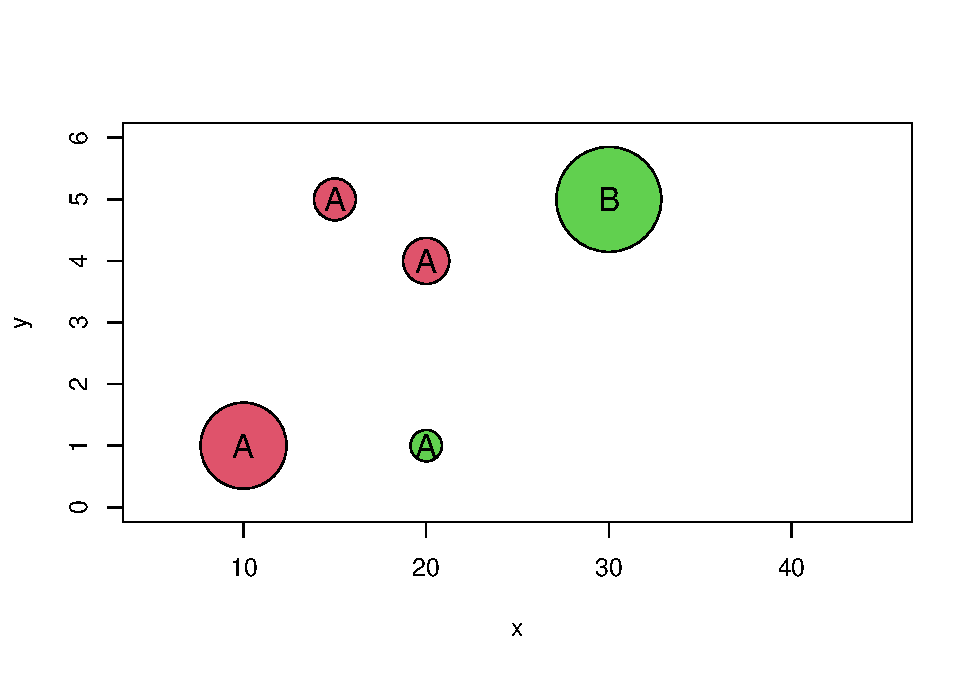
\includegraphics{AED_files/figure-latex/unnamed-chunk-2-1} \end{center}

\begin{center}\rule{0.5\linewidth}{0.5pt}\end{center}

\section{Diferentes gráficos de barras}\label{diferentes-gruxe1ficos-de-barras}

\subsection{Barras agrupadas}\label{barras-agrupadas}

\begin{Shaded}
\begin{Highlighting}[]
\NormalTok{ano}\OtherTok{=}\FunctionTok{c}\NormalTok{(}\FunctionTok{rep}\NormalTok{(}\DecValTok{2022}\NormalTok{,}\DecValTok{12}\NormalTok{),}\FunctionTok{rep}\NormalTok{(}\DecValTok{2023}\NormalTok{,}\DecValTok{12}\NormalTok{))}
\NormalTok{mes}\OtherTok{=}\FunctionTok{c}\NormalTok{(}\FunctionTok{rep}\NormalTok{(}\DecValTok{1}\SpecialCharTok{:}\DecValTok{12}\NormalTok{,}\DecValTok{2}\NormalTok{))}
\NormalTok{vendas}\OtherTok{=}\FunctionTok{rpois}\NormalTok{(}\DecValTok{24}\NormalTok{,}\DecValTok{15}\NormalTok{)}
\NormalTok{m }\OtherTok{\textless{}{-}} \FunctionTok{c}\NormalTok{(}\StringTok{\textquotesingle{}Jan\textquotesingle{}}\NormalTok{,}\StringTok{\textquotesingle{}Fev\textquotesingle{}}\NormalTok{,}\StringTok{\textquotesingle{}Mar\textquotesingle{}}\NormalTok{,}\StringTok{\textquotesingle{}Abr\textquotesingle{}}\NormalTok{,}\StringTok{\textquotesingle{}Mai\textquotesingle{}}\NormalTok{,}\StringTok{\textquotesingle{}Jun\textquotesingle{}}\NormalTok{,}
       \StringTok{\textquotesingle{}Jul\textquotesingle{}}\NormalTok{,}\StringTok{\textquotesingle{}Ago\textquotesingle{}}\NormalTok{,}\StringTok{\textquotesingle{}Set\textquotesingle{}}\NormalTok{,}\StringTok{\textquotesingle{}Out\textquotesingle{}}\NormalTok{,}\StringTok{\textquotesingle{}Nov\textquotesingle{}}\NormalTok{,}\StringTok{\textquotesingle{}Dez\textquotesingle{}}\NormalTok{)}
\NormalTok{cores}\OtherTok{=}\FunctionTok{c}\NormalTok{(}\StringTok{"deeppink3"}\NormalTok{,}\StringTok{"pink"}\NormalTok{)}

\FunctionTok{barplot}\NormalTok{(}\FunctionTok{rbind}\NormalTok{(vendas[}\DecValTok{1}\SpecialCharTok{:}\DecValTok{12}\NormalTok{],vendas[}\DecValTok{13}\SpecialCharTok{:}\DecValTok{24}\NormalTok{]),}
        \AttributeTok{beside=}\NormalTok{T,}\AttributeTok{names.arg =}\NormalTok{ m, }\AttributeTok{ylim=}\FunctionTok{c}\NormalTok{(}\DecValTok{0}\NormalTok{,}\DecValTok{25}\NormalTok{),}
        \AttributeTok{col=}\NormalTok{cores,}\AttributeTok{border=}\ConstantTok{NA}\NormalTok{,}\AttributeTok{ylab=}\StringTok{"Vendas"}\NormalTok{)}

\FunctionTok{legend}\NormalTok{(}\StringTok{\textquotesingle{}topright\textquotesingle{}}\NormalTok{,}\FunctionTok{c}\NormalTok{(}\StringTok{\textquotesingle{}2022\textquotesingle{}}\NormalTok{,}\StringTok{\textquotesingle{}2023\textquotesingle{}}\NormalTok{),}
       \AttributeTok{pch=}\DecValTok{15}\NormalTok{,}\AttributeTok{col=}\NormalTok{cores,}\AttributeTok{box.col=}\ConstantTok{NA}\NormalTok{)}
\end{Highlighting}
\end{Shaded}

\begin{center}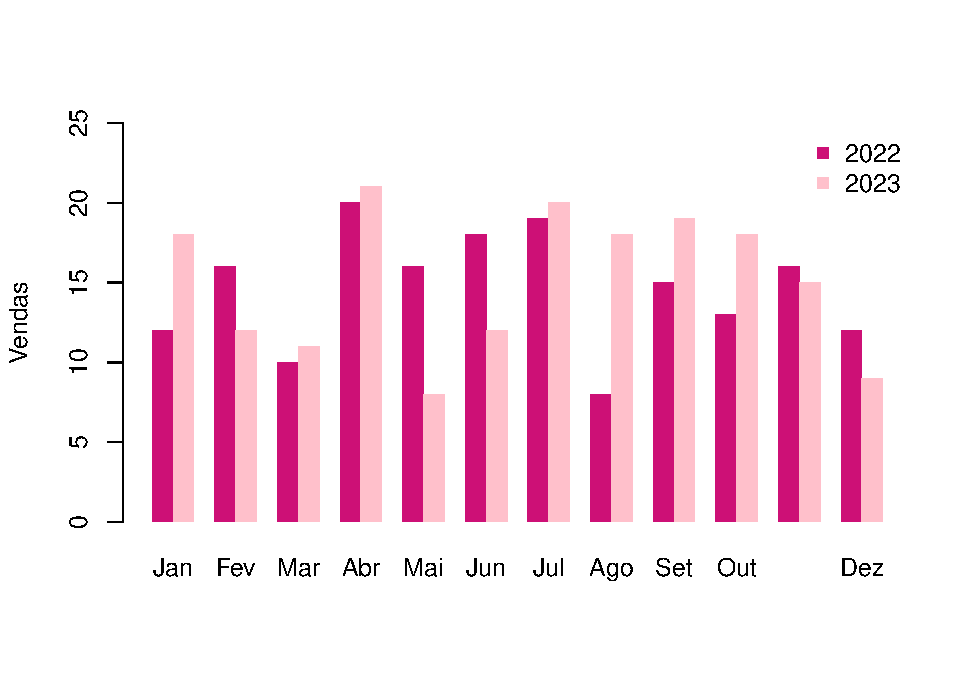
\includegraphics{AED_files/figure-latex/unnamed-chunk-3-1} \end{center}

\subsection{Barras empilhadas}\label{barras-empilhadas}

\subsection{Barras 100\% empilhadas}\label{barras-100-empilhadas}

\begin{center}\rule{0.5\linewidth}{0.5pt}\end{center}

\section{Gráfico de velocímetro}\label{gruxe1fico-de-velocuxedmetro}

\begin{center}\rule{0.5\linewidth}{0.5pt}\end{center}

\section{Gráfico mosaíco}\label{gruxe1fico-mosauxedco}

\begin{center}\rule{0.5\linewidth}{0.5pt}\end{center}

\section{Nuvem de palavras}\label{nuvem-de-palavras}

\begin{center}\rule{0.5\linewidth}{0.5pt}\end{center}

\section{Configurações gráficas}\label{configurauxe7uxf5es-gruxe1ficas}

\subsection{Cor de fundo}\label{cor-de-fundo}

\subsection{Imagem de fundo}\label{imagem-de-fundo}

\subsection{Margens gráficas}\label{margens-gruxe1ficas}

\subsection{Janelas multiplas}\label{janelas-multiplas}

\begin{center}\rule{0.5\linewidth}{0.5pt}\end{center}

\section{Exercício}\label{exercuxedcio}

\chapter{Regressão linear (incompleto)}\label{regressuxe3o-linear-incompleto}

A regressão linear modela a relação entre duas variáveis quantitativas, onde uma variável é considerada dependente e a outra é independente. O objetivo principal é estabelecer uma equação linear que descreva como a variável dependente (\(Y\)) se comporta em função da variável independente.

A equação da regressão linear simples é \(Y = a + b X + \varepsilon\).

Onde:
- \(Y\) é a variável resposta (dependente)
- \(X\) é a variável explicativa (independente)
- \(a\) é o intercepto (valor de \(Y\) quando \(X = 0\))
- \(b\) é o coeficiente angular (indica a variação de \(Y\) para cada unidade de \(X\))
- \(\varepsilon\)é um erro aleatório.

\begin{center}\rule{0.5\linewidth}{0.5pt}\end{center}

Suponha que temos interesse em estudar o valor esperado do peso de uma pessoa (\(Y\), em kg), com base em sua altura (\(X\), em cm). Para isso, coletamos dados de várias pessoas e ajustamos um modelo de regressão linear.

\begin{verbatim}
## Warning: Using `size` aesthetic for lines was deprecated in ggplot2 3.4.0.
## i Please use `linewidth` instead.
## This warning is displayed once every 8 hours.
## Call `lifecycle::last_lifecycle_warnings()` to see where this warning was
## generated.
\end{verbatim}

\begin{verbatim}
## `geom_smooth()` using formula = 'y ~ x'
\end{verbatim}

\begin{center}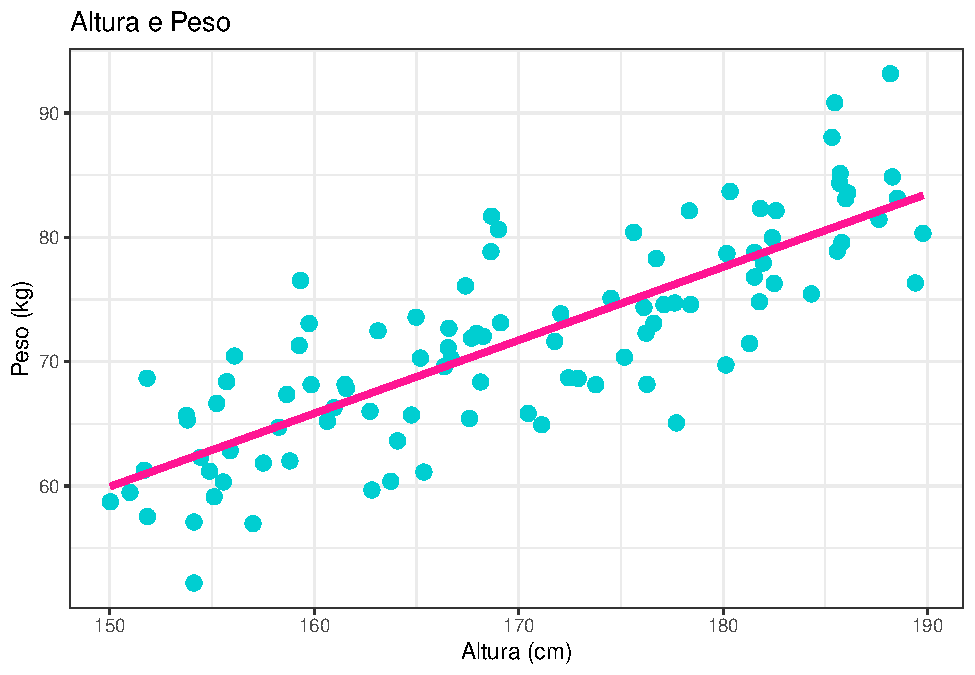
\includegraphics{AED_files/figure-latex/graf_regrecao-1} \end{center}

\(Y\): Variável resposta (dependente)
\(X\): Variável explicativa (independente)

Com isso, temos que,

\[
E[Y \mid X = x] = a + bx
\]

Agora, para conseguir estimar esse valor esperado do peso de uma pessoa, com base em sua altura, precisamos obter o valor \(a\) e \(b\).

\begin{center}\rule{0.5\linewidth}{0.5pt}\end{center}

\section{\texorpdfstring{Estimar \(a\) e \(b\)}{Estimar a e b}}\label{estimar-a-e-b}

Para estimar os coeficientes usamos o método dos mínimos quadrados

\[
S = \sum_{i=1}^{n} e_i^2 = \sum_{i=1}^{n} (y_i - (a + bx_i))^2 = \sum_{i=1}^{n} (y_i - a - bx_i)^2\\
\]

\[
\left\{
  \begin{array}{l}
    \frac{\partial S(a, b)}{\partial a} = 0 \\
    \frac{\partial S(a, b)}{\partial b} = 0
  \end{array}
\right.
\Longrightarrow
\left\{
  \begin{array}{l}
    \frac{\partial S(a, b)}{\partial a} = - \sum_{i=1}^{n} 2(y_i - a - b x_i) = 0 \\
    \frac{\partial S(a, b)}{\partial b} = - \sum_{i=1}^{n} x_i \cdot 2(y_i - a - b x_i) = 0
  \end{array}
\right.
\]

\[
\Longrightarrow 
- \sum_{i=1}^{n} y_i + n a + b \sum_{i=1}^{n} x_i = 0
\Longrightarrow
a = \frac{\sum_{i=1}^{n} y_i}{n} - b \frac{\sum_{i=1}^{n} x_i}{n}
\]
\[
\Longrightarrow
a = \bar{y} - b\bar{x}
\]

  \bibliography{book.bib,packages.bib}

\end{document}
